\chapter{Appendix}

        \section{PP}
        
                \subsection*{PP Yields and Ratios}
                \begin{figure}[H]
                    \title{Region Inclusive}
                    \begin{subfigure}[b]{0.5\textwidth}
                        \centering
                        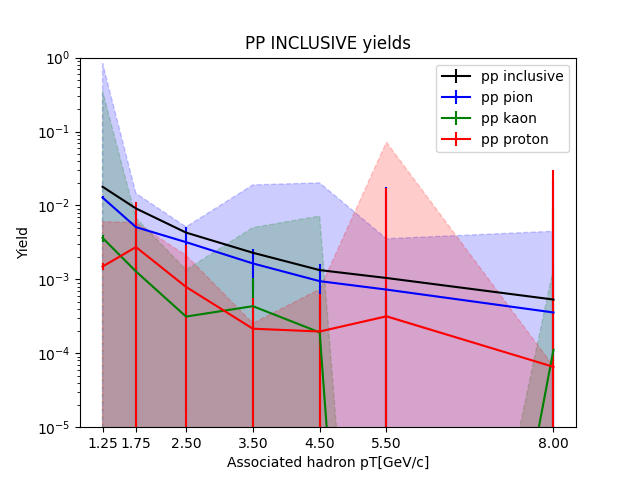
\includegraphics[width=\textwidth]{figures/png/appendix_plots/PP/Region.INCLUSIVE_yields.png}
                        \caption{Particle yields for PP INCLUSIVE region.}
                        \label{fig:appendix_PP_INCLUSIVE_Inclusive_Yields}
                    \end{subfigure}
                    \begin{subfigure}[b]{0.5\textwidth}
                        \centering
                        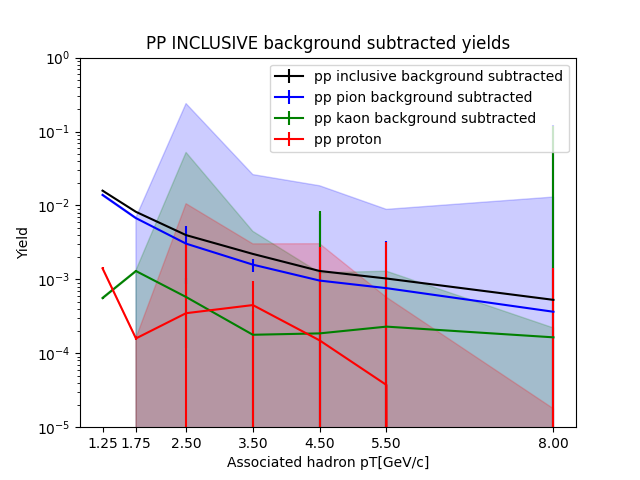
\includegraphics[width=\textwidth]{figures/png/appendix_plots/PP/Region.INCLUSIVE_background_subtracted_yields.png}
                        \caption{Particle yields for PP INCLUSIVE region with background subtracted.}
                        \label{fig:appendix_PP_INCLUSIVE_Inclusive_Yields_Background_Subtracted}
                    \end{subfigure}
                    \begin{subfigure}[b]{0.5\textwidth}
                        \centering
                        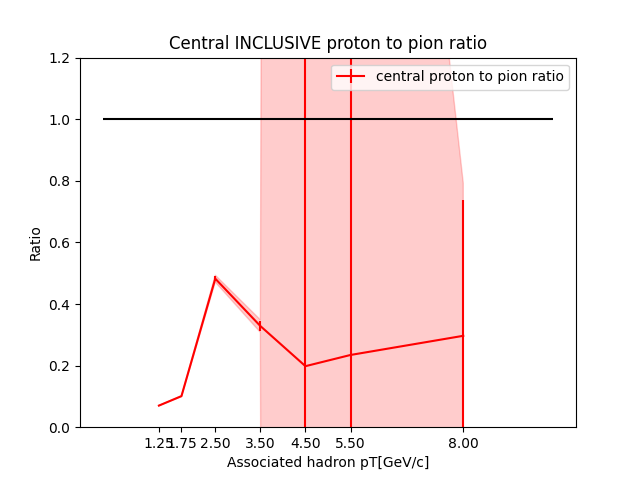
\includegraphics[width=\textwidth]{figures/png/appendix_plots/PP/Region.INCLUSIVE_proton_to_pion_ratio.png}
                        \caption{Proton to Pion ratio for PP INCLUSIVE region.}
                        \label{fig:appendix_PP_INCLUSIVE_Proton_to_Pion_Ratio}
                    \end{subfigure}
                    \begin{subfigure}[b]{0.5\textwidth}
                        \centering
                        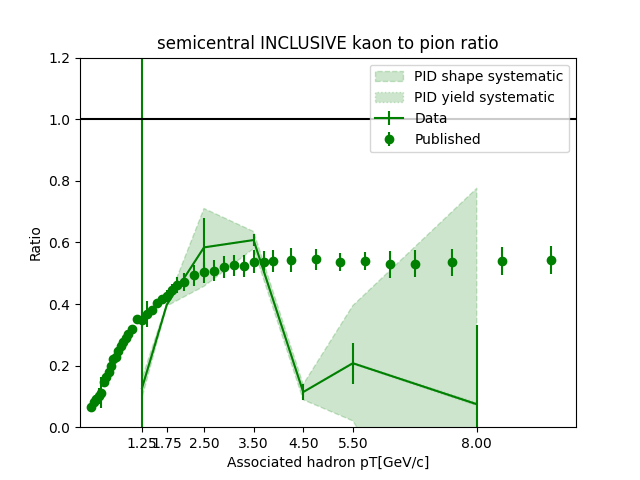
\includegraphics[width=\textwidth]{figures/png/appendix_plots/PP/Region.INCLUSIVE_kaon_to_pion_ratio.png}
                        \caption{Kaon to Pion ratio for PP INCLUSIVE region.}
                        \label{fig:appendix_PP_INCLUSIVE_Kaon_to_Pion_Ratio}
                    \end{subfigure}
                    \caption{Particle yields and ratios for PP INCLUSIVE region.}
                    \label{fig:appendix_PP_INCLUSIVE_Inclusive_Yields_and_Ratios}
                \end{figure}
                \begin{figure}[H]
                    \title{Region Near-side}
                    \begin{subfigure}[b]{0.5\textwidth}
                        \centering
                        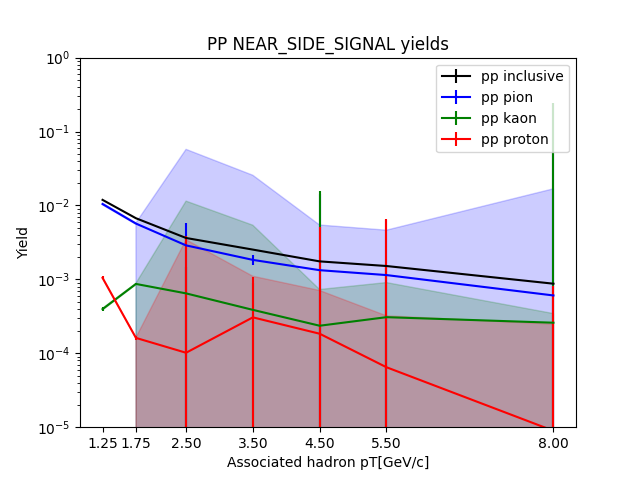
\includegraphics[width=\textwidth]{figures/png/appendix_plots/PP/Region.NEAR_SIDE_SIGNAL_yields.png}
                        \caption{Particle yields for PP NEAR-SIDE region.}
                        \label{fig:appendix_PP_NEAR_SIDE_SIGNAL_Inclusive_Yields}
                    \end{subfigure}
                    \begin{subfigure}[b]{0.5\textwidth}
                        \centering
                        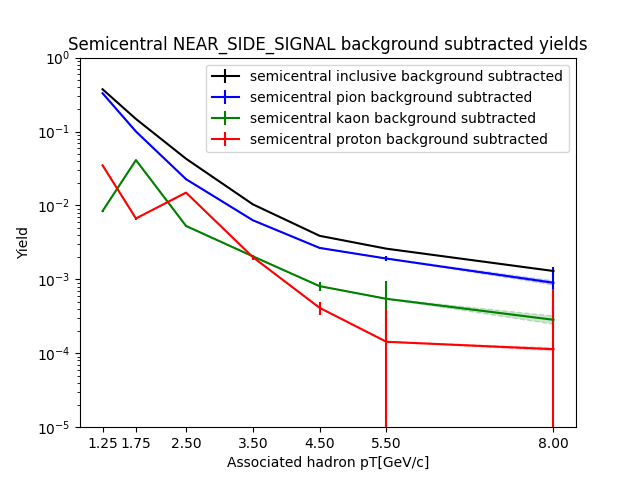
\includegraphics[width=\textwidth]{figures/png/appendix_plots/PP/Region.NEAR_SIDE_SIGNAL_background_subtracted_yields.png}
                        \caption{Particle yields for PP NEAR-SIDE region with background subtracted.}
                        \label{fig:appendix_PP_NEAR_SIDE_SIGNAL_Inclusive_Yields_Background_Subtracted}
                    \end{subfigure}
                    \begin{subfigure}[b]{0.5\textwidth}
                        \centering
                        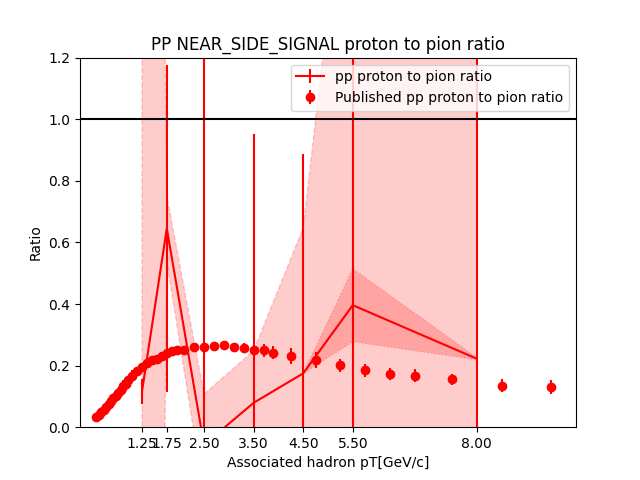
\includegraphics[width=\textwidth]{figures/png/appendix_plots/PP/Region.NEAR_SIDE_SIGNAL_proton_to_pion_ratio.png}
                        \caption{Proton to Pion ratio for PP NEAR-SIDE region.}
                        \label{fig:appendix_PP_NEAR_SIDE_SIGNAL_Proton_to_Pion_Ratio}
                    \end{subfigure}
                    \begin{subfigure}[b]{0.5\textwidth}
                        \centering
                        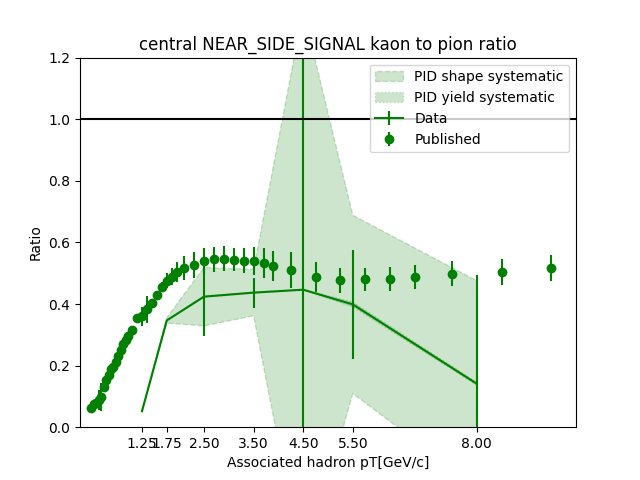
\includegraphics[width=\textwidth]{figures/png/appendix_plots/PP/Region.NEAR_SIDE_SIGNAL_kaon_to_pion_ratio.png}
                        \caption{Kaon to Pion ratio for PP NEAR-SIDE region.}
                        \label{fig:appendix_PP_NEAR_SIDE_SIGNAL_Kaon_to_Pion_Ratio}
                    \end{subfigure}
                    \caption{Particle yields and ratios for PP NEAR-SIDE region.}
                    \label{fig:appendix_PP_NEAR_SIDE_SIGNAL_Inclusive_Yields_and_Ratios}
                \end{figure}
                \begin{figure}[H]
                    \title{Region Away-side}
                    \begin{subfigure}[b]{0.5\textwidth}
                        \centering
                        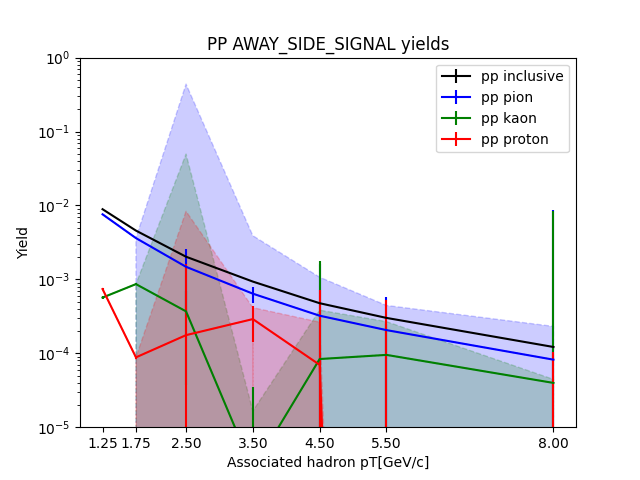
\includegraphics[width=\textwidth]{figures/png/appendix_plots/PP/Region.AWAY_SIDE_SIGNAL_yields.png}
                        \caption{Particle yields for PP AWAY-SIDE region.}
                        \label{fig:appendix_PP_AWAY_SIDE_SIGNAL_Inclusive_Yields}
                    \end{subfigure}
                    \begin{subfigure}[b]{0.5\textwidth}
                        \centering
                        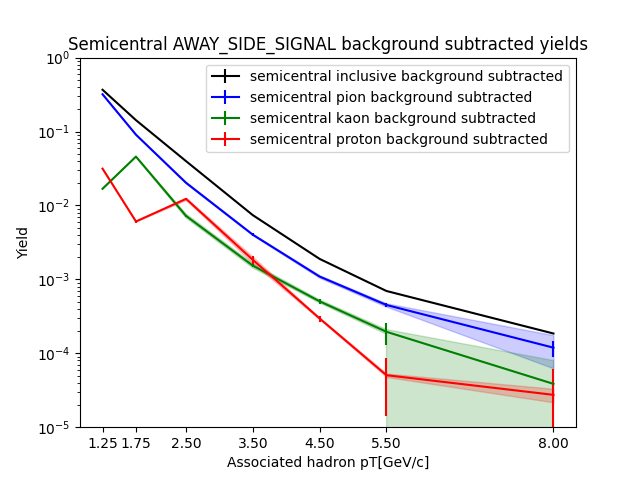
\includegraphics[width=\textwidth]{figures/png/appendix_plots/PP/Region.AWAY_SIDE_SIGNAL_background_subtracted_yields.png}
                        \caption{Particle yields for PP AWAY-SIDE region with background subtracted.}
                        \label{fig:appendix_PP_AWAY_SIDE_SIGNAL_Inclusive_Yields_Background_Subtracted}
                    \end{subfigure}
                    \begin{subfigure}[b]{0.5\textwidth}
                        \centering
                        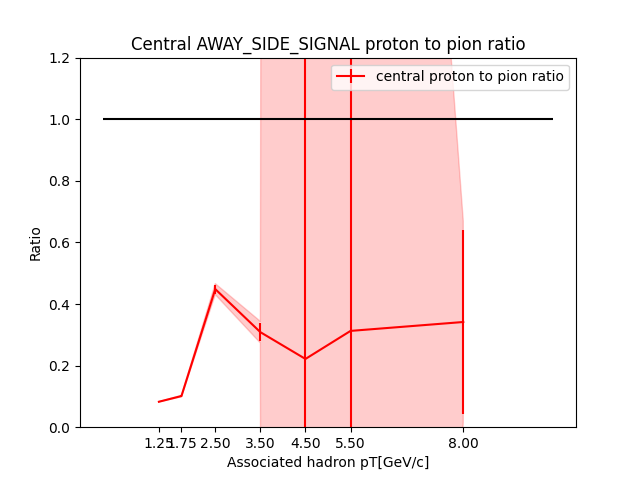
\includegraphics[width=\textwidth]{figures/png/appendix_plots/PP/Region.AWAY_SIDE_SIGNAL_proton_to_pion_ratio.png}
                        \caption{Proton to Pion ratio for PP AWAY-SIDE region.}
                        \label{fig:appendix_PP_AWAY_SIDE_SIGNAL_Proton_to_Pion_Ratio}
                    \end{subfigure}
                    \begin{subfigure}[b]{0.5\textwidth}
                        \centering
                        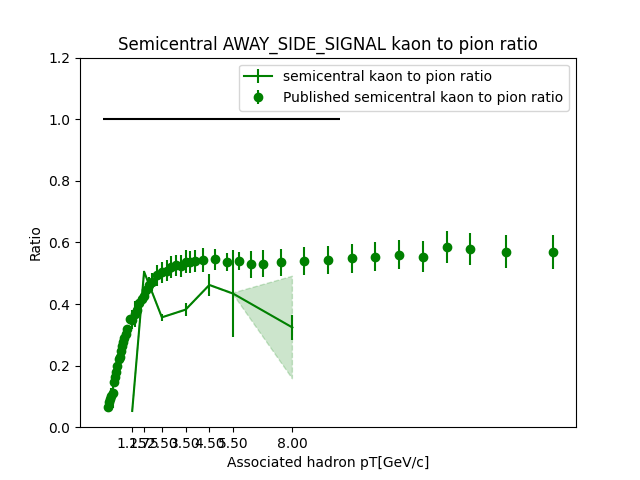
\includegraphics[width=\textwidth]{figures/png/appendix_plots/PP/Region.AWAY_SIDE_SIGNAL_kaon_to_pion_ratio.png}
                        \caption{Kaon to Pion ratio for PP AWAY-SIDE region.}
                        \label{fig:appendix_PP_AWAY_SIDE_SIGNAL_Kaon_to_Pion_Ratio}
                    \end{subfigure}
                    \caption{Particle yields and ratios for PP AWAY-SIDE region.}
                    \label{fig:appendix_PP_AWAY_SIDE_SIGNAL_Inclusive_Yields_and_Ratios}
                \end{figure}
                \begin{figure}[H]
                    \title{Region Background}
                    \begin{subfigure}[b]{0.5\textwidth}
                        \centering
                        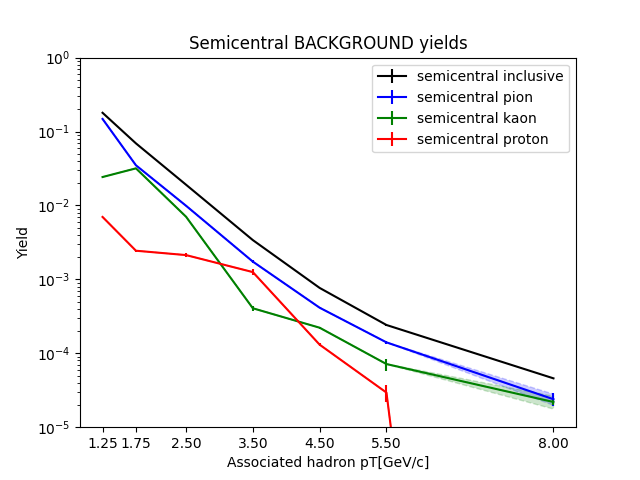
\includegraphics[width=\textwidth]{figures/png/appendix_plots/PP/Region.BACKGROUND_yields.png}
                        \caption{Particle yields for PP BACKGROUND region.}
                        \label{fig:appendix_PP_BACKGROUND_Inclusive_Yields}
                    \end{subfigure}
                    \caption{Particle yields for PP BACKGROUND region.}
                    \label{fig:appendix_PP_BACKGROUND_Inclusive_Yields}
                \end{figure}


    
            \subsection*{PP $1 < \pTassoc < 1.5$ GeV/c}
            \begin{figure}[H]
                \title{Region Inclusive}
                \begin{subfigure}[b]{0.5\textwidth}
                    \centering
                    \includegraphics[width=\textwidth]{figures/png/appendix_plots/PP/PT_1_15/TPCnSigmaFits/TPCnSigmaFit_Region.INCLUSIVE_Inclusive.png}
                    \caption{TPC n$\sigma$ fits for PP $1 < \pTassoc < 1.5$ GeV/c INCLUSIVE region for Inclusive particles.}
                    \label{fig:appendix_PP_$1 < \pTassoc < 1.5$ GeV/c_INCLUSIVE_Inclusive}
                \end{subfigure}
                \begin{subfigure}[b]{0.5\textwidth}
                    \centering
                    \includegraphics[width=\textwidth]{figures/png/appendix_plots/PP/PT_1_15/TPCnSigmaFits/TPCnSigmaFit_Region.INCLUSIVE_Pion.png}
                    \caption{TPC n$\sigma$ fits for PP $1 < \pTassoc < 1.5$ GeV/c INCLUSIVE region for Pions.}
                    \label{fig:appendix_PP_$1 < \pTassoc < 1.5$ GeV/c_INCLUSIVE_Pion}
                \end{subfigure}
                \begin{subfigure}[b]{0.5\textwidth}
                    \centering
                    \includegraphics[width=\textwidth]{figures/png/appendix_plots/PP/PT_1_15/TPCnSigmaFits/TPCnSigmaFit_Region.INCLUSIVE_Proton.png}
                    \caption{TPC n$\sigma$ fits for PP $1 < \pTassoc < 1.5$ GeV/c INCLUSIVE region for Protons.}
                    \label{fig:appendix_PP_$1 < \pTassoc < 1.5$ GeV/c_INCLUSIVE_Proton}
                \end{subfigure}
                \begin{subfigure}[b]{0.5\textwidth}
                    \centering
                    \includegraphics[width=\textwidth]{figures/png/appendix_plots/PP/PT_1_15/TPCnSigmaFits/TPCnSigmaFit_Region.INCLUSIVE_Kaon.png}
                    \caption{TPC n$\sigma$ fits for PP $1 < \pTassoc < 1.5$ GeV/c INCLUSIVE region for Kaons.}
                    \label{fig:appendix_PP_$1 < \pTassoc < 1.5$ GeV/c_INCLUSIVE_Kaon}
                \end{subfigure}
                \caption{TPC n$\sigma$ fits for PP $1 < \pTassoc < 1.5$ GeV/c INCLUSIVE region.}
                \label{fig:appendix_PP_$1 < \pTassoc < 1.5$ GeV/c_INCLUSIVE}
            \end{figure}
            \begin{figure}[H]
                \title{Region Near-side}
                \begin{subfigure}[b]{0.5\textwidth}
                    \centering
                    \includegraphics[width=\textwidth]{figures/png/appendix_plots/PP/PT_1_15/TPCnSigmaFits/TPCnSigmaFit_Region.NEAR_SIDE_SIGNAL_Inclusive.png}
                    \caption{TPC n$\sigma$ fits for PP $1 < \pTassoc < 1.5$ GeV/c NEAR-SIDE region for Inclusive particles.}
                    \label{fig:appendix_PP_$1 < \pTassoc < 1.5$ GeV/c_NEAR_SIDE_SIGNAL_Inclusive}
                \end{subfigure}
                \begin{subfigure}[b]{0.5\textwidth}
                    \centering
                    \includegraphics[width=\textwidth]{figures/png/appendix_plots/PP/PT_1_15/TPCnSigmaFits/TPCnSigmaFit_Region.NEAR_SIDE_SIGNAL_Pion.png}
                    \caption{TPC n$\sigma$ fits for PP $1 < \pTassoc < 1.5$ GeV/c NEAR-SIDE region for Pions.}
                    \label{fig:appendix_PP_$1 < \pTassoc < 1.5$ GeV/c_NEAR_SIDE_SIGNAL_Pion}
                \end{subfigure}
                \begin{subfigure}[b]{0.5\textwidth}
                    \centering
                    \includegraphics[width=\textwidth]{figures/png/appendix_plots/PP/PT_1_15/TPCnSigmaFits/TPCnSigmaFit_Region.NEAR_SIDE_SIGNAL_Proton.png}
                    \caption{TPC n$\sigma$ fits for PP $1 < \pTassoc < 1.5$ GeV/c NEAR-SIDE region for Protons.}
                    \label{fig:appendix_PP_$1 < \pTassoc < 1.5$ GeV/c_NEAR_SIDE_SIGNAL_Proton}
                \end{subfigure}
                \begin{subfigure}[b]{0.5\textwidth}
                    \centering
                    \includegraphics[width=\textwidth]{figures/png/appendix_plots/PP/PT_1_15/TPCnSigmaFits/TPCnSigmaFit_Region.NEAR_SIDE_SIGNAL_Kaon.png}
                    \caption{TPC n$\sigma$ fits for PP $1 < \pTassoc < 1.5$ GeV/c NEAR-SIDE region for Kaons.}
                    \label{fig:appendix_PP_$1 < \pTassoc < 1.5$ GeV/c_NEAR_SIDE_SIGNAL_Kaon}
                \end{subfigure}
                \caption{TPC n$\sigma$ fits for PP $1 < \pTassoc < 1.5$ GeV/c NEAR-SIDE region.}
                \label{fig:appendix_PP_$1 < \pTassoc < 1.5$ GeV/c_NEAR_SIDE_SIGNAL}
            \end{figure}
            \begin{figure}[H]
                \title{Region Away-side}
                \begin{subfigure}[b]{0.5\textwidth}
                    \centering
                    \includegraphics[width=\textwidth]{figures/png/appendix_plots/PP/PT_1_15/TPCnSigmaFits/TPCnSigmaFit_Region.AWAY_SIDE_SIGNAL_Inclusive.png}
                    \caption{TPC n$\sigma$ fits for PP $1 < \pTassoc < 1.5$ GeV/c AWAY-SIDE region for Inclusive particles.}
                    \label{fig:appendix_PP_$1 < \pTassoc < 1.5$ GeV/c_AWAY_SIDE_SIGNAL_Inclusive}
                \end{subfigure}
                \begin{subfigure}[b]{0.5\textwidth}
                    \centering
                    \includegraphics[width=\textwidth]{figures/png/appendix_plots/PP/PT_1_15/TPCnSigmaFits/TPCnSigmaFit_Region.AWAY_SIDE_SIGNAL_Pion.png}
                    \caption{TPC n$\sigma$ fits for PP $1 < \pTassoc < 1.5$ GeV/c AWAY-SIDE region for Pions.}
                    \label{fig:appendix_PP_$1 < \pTassoc < 1.5$ GeV/c_AWAY_SIDE_SIGNAL_Pion}
                \end{subfigure}
                \begin{subfigure}[b]{0.5\textwidth}
                    \centering
                    \includegraphics[width=\textwidth]{figures/png/appendix_plots/PP/PT_1_15/TPCnSigmaFits/TPCnSigmaFit_Region.AWAY_SIDE_SIGNAL_Proton.png}
                    \caption{TPC n$\sigma$ fits for PP $1 < \pTassoc < 1.5$ GeV/c AWAY-SIDE region for Protons.}
                    \label{fig:appendix_PP_$1 < \pTassoc < 1.5$ GeV/c_AWAY_SIDE_SIGNAL_Proton}
                \end{subfigure}
                \begin{subfigure}[b]{0.5\textwidth}
                    \centering
                    \includegraphics[width=\textwidth]{figures/png/appendix_plots/PP/PT_1_15/TPCnSigmaFits/TPCnSigmaFit_Region.AWAY_SIDE_SIGNAL_Kaon.png}
                    \caption{TPC n$\sigma$ fits for PP $1 < \pTassoc < 1.5$ GeV/c AWAY-SIDE region for Kaons.}
                    \label{fig:appendix_PP_$1 < \pTassoc < 1.5$ GeV/c_AWAY_SIDE_SIGNAL_Kaon}
                \end{subfigure}
                \caption{TPC n$\sigma$ fits for PP $1 < \pTassoc < 1.5$ GeV/c AWAY-SIDE region.}
                \label{fig:appendix_PP_$1 < \pTassoc < 1.5$ GeV/c_AWAY_SIDE_SIGNAL}
            \end{figure}
            \begin{figure}[H]
                \title{Region Background}
                \begin{subfigure}[b]{0.5\textwidth}
                    \centering
                    \includegraphics[width=\textwidth]{figures/png/appendix_plots/PP/PT_1_15/TPCnSigmaFits/TPCnSigmaFit_Region.BACKGROUND_Inclusive.png}
                    \caption{TPC n$\sigma$ fits for PP $1 < \pTassoc < 1.5$ GeV/c BACKGROUND region for Inclusive particles.}
                    \label{fig:appendix_PP_$1 < \pTassoc < 1.5$ GeV/c_BACKGROUND_Inclusive}
                \end{subfigure}
                \begin{subfigure}[b]{0.5\textwidth}
                    \centering
                    \includegraphics[width=\textwidth]{figures/png/appendix_plots/PP/PT_1_15/TPCnSigmaFits/TPCnSigmaFit_Region.BACKGROUND_Pion.png}
                    \caption{TPC n$\sigma$ fits for PP $1 < \pTassoc < 1.5$ GeV/c BACKGROUND region for Pions.}
                    \label{fig:appendix_PP_$1 < \pTassoc < 1.5$ GeV/c_BACKGROUND_Pion}
                \end{subfigure}
                \begin{subfigure}[b]{0.5\textwidth}
                    \centering
                    \includegraphics[width=\textwidth]{figures/png/appendix_plots/PP/PT_1_15/TPCnSigmaFits/TPCnSigmaFit_Region.BACKGROUND_Proton.png}
                    \caption{TPC n$\sigma$ fits for PP $1 < \pTassoc < 1.5$ GeV/c BACKGROUND region for Protons.}
                    \label{fig:appendix_PP_$1 < \pTassoc < 1.5$ GeV/c_BACKGROUND_Proton}
                \end{subfigure}
                \begin{subfigure}[b]{0.5\textwidth}
                    \centering
                    \includegraphics[width=\textwidth]{figures/png/appendix_plots/PP/PT_1_15/TPCnSigmaFits/TPCnSigmaFit_Region.BACKGROUND_Kaon.png}
                    \caption{TPC n$\sigma$ fits for PP $1 < \pTassoc < 1.5$ GeV/c BACKGROUND region for Kaons.}
                    \label{fig:appendix_PP_$1 < \pTassoc < 1.5$ GeV/c_BACKGROUND_Kaon}
                \end{subfigure}
                \caption{TPC n$\sigma$ fits for PP $1 < \pTassoc < 1.5$ GeV/c BACKGROUND region.}
                \label{fig:appendix_PP_$1 < \pTassoc < 1.5$ GeV/c_BACKGROUND}
            \end{figure}
            \clearpage
            
    
            \subsection*{PP $1.5 < \pTassoc < 2$ GeV/c}
            \begin{figure}[H]
                \title{Region Inclusive}
                \begin{subfigure}[b]{0.5\textwidth}
                    \centering
                    \includegraphics[width=\textwidth]{figures/png/appendix_plots/PP/PT_15_2/TPCnSigmaFits/TPCnSigmaFit_Region.INCLUSIVE_Inclusive.png}
                    \caption{TPC n$\sigma$ fits for PP $1.5 < \pTassoc < 2$ GeV/c INCLUSIVE region for Inclusive particles.}
                    \label{fig:appendix_PP_$1.5 < \pTassoc < 2$ GeV/c_INCLUSIVE_Inclusive}
                \end{subfigure}
                \begin{subfigure}[b]{0.5\textwidth}
                    \centering
                    \includegraphics[width=\textwidth]{figures/png/appendix_plots/PP/PT_15_2/TPCnSigmaFits/TPCnSigmaFit_Region.INCLUSIVE_Pion.png}
                    \caption{TPC n$\sigma$ fits for PP $1.5 < \pTassoc < 2$ GeV/c INCLUSIVE region for Pions.}
                    \label{fig:appendix_PP_$1.5 < \pTassoc < 2$ GeV/c_INCLUSIVE_Pion}
                \end{subfigure}
                \begin{subfigure}[b]{0.5\textwidth}
                    \centering
                    \includegraphics[width=\textwidth]{figures/png/appendix_plots/PP/PT_15_2/TPCnSigmaFits/TPCnSigmaFit_Region.INCLUSIVE_Proton.png}
                    \caption{TPC n$\sigma$ fits for PP $1.5 < \pTassoc < 2$ GeV/c INCLUSIVE region for Protons.}
                    \label{fig:appendix_PP_$1.5 < \pTassoc < 2$ GeV/c_INCLUSIVE_Proton}
                \end{subfigure}
                \begin{subfigure}[b]{0.5\textwidth}
                    \centering
                    \includegraphics[width=\textwidth]{figures/png/appendix_plots/PP/PT_15_2/TPCnSigmaFits/TPCnSigmaFit_Region.INCLUSIVE_Kaon.png}
                    \caption{TPC n$\sigma$ fits for PP $1.5 < \pTassoc < 2$ GeV/c INCLUSIVE region for Kaons.}
                    \label{fig:appendix_PP_$1.5 < \pTassoc < 2$ GeV/c_INCLUSIVE_Kaon}
                \end{subfigure}
                \caption{TPC n$\sigma$ fits for PP $1.5 < \pTassoc < 2$ GeV/c INCLUSIVE region.}
                \label{fig:appendix_PP_$1.5 < \pTassoc < 2$ GeV/c_INCLUSIVE}
            \end{figure}
            \begin{figure}[H]
                \title{Region Near-side}
                \begin{subfigure}[b]{0.5\textwidth}
                    \centering
                    \includegraphics[width=\textwidth]{figures/png/appendix_plots/PP/PT_15_2/TPCnSigmaFits/TPCnSigmaFit_Region.NEAR_SIDE_SIGNAL_Inclusive.png}
                    \caption{TPC n$\sigma$ fits for PP $1.5 < \pTassoc < 2$ GeV/c NEAR-SIDE region for Inclusive particles.}
                    \label{fig:appendix_PP_$1.5 < \pTassoc < 2$ GeV/c_NEAR_SIDE_SIGNAL_Inclusive}
                \end{subfigure}
                \begin{subfigure}[b]{0.5\textwidth}
                    \centering
                    \includegraphics[width=\textwidth]{figures/png/appendix_plots/PP/PT_15_2/TPCnSigmaFits/TPCnSigmaFit_Region.NEAR_SIDE_SIGNAL_Pion.png}
                    \caption{TPC n$\sigma$ fits for PP $1.5 < \pTassoc < 2$ GeV/c NEAR-SIDE region for Pions.}
                    \label{fig:appendix_PP_$1.5 < \pTassoc < 2$ GeV/c_NEAR_SIDE_SIGNAL_Pion}
                \end{subfigure}
                \begin{subfigure}[b]{0.5\textwidth}
                    \centering
                    \includegraphics[width=\textwidth]{figures/png/appendix_plots/PP/PT_15_2/TPCnSigmaFits/TPCnSigmaFit_Region.NEAR_SIDE_SIGNAL_Proton.png}
                    \caption{TPC n$\sigma$ fits for PP $1.5 < \pTassoc < 2$ GeV/c NEAR-SIDE region for Protons.}
                    \label{fig:appendix_PP_$1.5 < \pTassoc < 2$ GeV/c_NEAR_SIDE_SIGNAL_Proton}
                \end{subfigure}
                \begin{subfigure}[b]{0.5\textwidth}
                    \centering
                    \includegraphics[width=\textwidth]{figures/png/appendix_plots/PP/PT_15_2/TPCnSigmaFits/TPCnSigmaFit_Region.NEAR_SIDE_SIGNAL_Kaon.png}
                    \caption{TPC n$\sigma$ fits for PP $1.5 < \pTassoc < 2$ GeV/c NEAR-SIDE region for Kaons.}
                    \label{fig:appendix_PP_$1.5 < \pTassoc < 2$ GeV/c_NEAR_SIDE_SIGNAL_Kaon}
                \end{subfigure}
                \caption{TPC n$\sigma$ fits for PP $1.5 < \pTassoc < 2$ GeV/c NEAR-SIDE region.}
                \label{fig:appendix_PP_$1.5 < \pTassoc < 2$ GeV/c_NEAR_SIDE_SIGNAL}
            \end{figure}
            \begin{figure}[H]
                \title{Region Away-side}
                \begin{subfigure}[b]{0.5\textwidth}
                    \centering
                    \includegraphics[width=\textwidth]{figures/png/appendix_plots/PP/PT_15_2/TPCnSigmaFits/TPCnSigmaFit_Region.AWAY_SIDE_SIGNAL_Inclusive.png}
                    \caption{TPC n$\sigma$ fits for PP $1.5 < \pTassoc < 2$ GeV/c AWAY-SIDE region for Inclusive particles.}
                    \label{fig:appendix_PP_$1.5 < \pTassoc < 2$ GeV/c_AWAY_SIDE_SIGNAL_Inclusive}
                \end{subfigure}
                \begin{subfigure}[b]{0.5\textwidth}
                    \centering
                    \includegraphics[width=\textwidth]{figures/png/appendix_plots/PP/PT_15_2/TPCnSigmaFits/TPCnSigmaFit_Region.AWAY_SIDE_SIGNAL_Pion.png}
                    \caption{TPC n$\sigma$ fits for PP $1.5 < \pTassoc < 2$ GeV/c AWAY-SIDE region for Pions.}
                    \label{fig:appendix_PP_$1.5 < \pTassoc < 2$ GeV/c_AWAY_SIDE_SIGNAL_Pion}
                \end{subfigure}
                \begin{subfigure}[b]{0.5\textwidth}
                    \centering
                    \includegraphics[width=\textwidth]{figures/png/appendix_plots/PP/PT_15_2/TPCnSigmaFits/TPCnSigmaFit_Region.AWAY_SIDE_SIGNAL_Proton.png}
                    \caption{TPC n$\sigma$ fits for PP $1.5 < \pTassoc < 2$ GeV/c AWAY-SIDE region for Protons.}
                    \label{fig:appendix_PP_$1.5 < \pTassoc < 2$ GeV/c_AWAY_SIDE_SIGNAL_Proton}
                \end{subfigure}
                \begin{subfigure}[b]{0.5\textwidth}
                    \centering
                    \includegraphics[width=\textwidth]{figures/png/appendix_plots/PP/PT_15_2/TPCnSigmaFits/TPCnSigmaFit_Region.AWAY_SIDE_SIGNAL_Kaon.png}
                    \caption{TPC n$\sigma$ fits for PP $1.5 < \pTassoc < 2$ GeV/c AWAY-SIDE region for Kaons.}
                    \label{fig:appendix_PP_$1.5 < \pTassoc < 2$ GeV/c_AWAY_SIDE_SIGNAL_Kaon}
                \end{subfigure}
                \caption{TPC n$\sigma$ fits for PP $1.5 < \pTassoc < 2$ GeV/c AWAY-SIDE region.}
                \label{fig:appendix_PP_$1.5 < \pTassoc < 2$ GeV/c_AWAY_SIDE_SIGNAL}
            \end{figure}
            \begin{figure}[H]
                \title{Region Background}
                \begin{subfigure}[b]{0.5\textwidth}
                    \centering
                    \includegraphics[width=\textwidth]{figures/png/appendix_plots/PP/PT_15_2/TPCnSigmaFits/TPCnSigmaFit_Region.BACKGROUND_Inclusive.png}
                    \caption{TPC n$\sigma$ fits for PP $1.5 < \pTassoc < 2$ GeV/c BACKGROUND region for Inclusive particles.}
                    \label{fig:appendix_PP_$1.5 < \pTassoc < 2$ GeV/c_BACKGROUND_Inclusive}
                \end{subfigure}
                \begin{subfigure}[b]{0.5\textwidth}
                    \centering
                    \includegraphics[width=\textwidth]{figures/png/appendix_plots/PP/PT_15_2/TPCnSigmaFits/TPCnSigmaFit_Region.BACKGROUND_Pion.png}
                    \caption{TPC n$\sigma$ fits for PP $1.5 < \pTassoc < 2$ GeV/c BACKGROUND region for Pions.}
                    \label{fig:appendix_PP_$1.5 < \pTassoc < 2$ GeV/c_BACKGROUND_Pion}
                \end{subfigure}
                \begin{subfigure}[b]{0.5\textwidth}
                    \centering
                    \includegraphics[width=\textwidth]{figures/png/appendix_plots/PP/PT_15_2/TPCnSigmaFits/TPCnSigmaFit_Region.BACKGROUND_Proton.png}
                    \caption{TPC n$\sigma$ fits for PP $1.5 < \pTassoc < 2$ GeV/c BACKGROUND region for Protons.}
                    \label{fig:appendix_PP_$1.5 < \pTassoc < 2$ GeV/c_BACKGROUND_Proton}
                \end{subfigure}
                \begin{subfigure}[b]{0.5\textwidth}
                    \centering
                    \includegraphics[width=\textwidth]{figures/png/appendix_plots/PP/PT_15_2/TPCnSigmaFits/TPCnSigmaFit_Region.BACKGROUND_Kaon.png}
                    \caption{TPC n$\sigma$ fits for PP $1.5 < \pTassoc < 2$ GeV/c BACKGROUND region for Kaons.}
                    \label{fig:appendix_PP_$1.5 < \pTassoc < 2$ GeV/c_BACKGROUND_Kaon}
                \end{subfigure}
                \caption{TPC n$\sigma$ fits for PP $1.5 < \pTassoc < 2$ GeV/c BACKGROUND region.}
                \label{fig:appendix_PP_$1.5 < \pTassoc < 2$ GeV/c_BACKGROUND}
            \end{figure}
            \clearpage
            
    
            \subsection*{PP $2 < \pTassoc < 3$ GeV/c}
            \begin{figure}[H]
                \title{Region Inclusive}
                \begin{subfigure}[b]{0.5\textwidth}
                    \centering
                    \includegraphics[width=\textwidth]{figures/png/appendix_plots/PP/PT_2_3/TPCnSigmaFits/TPCnSigmaFit_Region.INCLUSIVE_Inclusive.png}
                    \caption{TPC n$\sigma$ fits for PP $2 < \pTassoc < 3$ GeV/c INCLUSIVE region for Inclusive particles.}
                    \label{fig:appendix_PP_$2 < \pTassoc < 3$ GeV/c_INCLUSIVE_Inclusive}
                \end{subfigure}
                \begin{subfigure}[b]{0.5\textwidth}
                    \centering
                    \includegraphics[width=\textwidth]{figures/png/appendix_plots/PP/PT_2_3/TPCnSigmaFits/TPCnSigmaFit_Region.INCLUSIVE_Pion.png}
                    \caption{TPC n$\sigma$ fits for PP $2 < \pTassoc < 3$ GeV/c INCLUSIVE region for Pions.}
                    \label{fig:appendix_PP_$2 < \pTassoc < 3$ GeV/c_INCLUSIVE_Pion}
                \end{subfigure}
                \begin{subfigure}[b]{0.5\textwidth}
                    \centering
                    \includegraphics[width=\textwidth]{figures/png/appendix_plots/PP/PT_2_3/TPCnSigmaFits/TPCnSigmaFit_Region.INCLUSIVE_Proton.png}
                    \caption{TPC n$\sigma$ fits for PP $2 < \pTassoc < 3$ GeV/c INCLUSIVE region for Protons.}
                    \label{fig:appendix_PP_$2 < \pTassoc < 3$ GeV/c_INCLUSIVE_Proton}
                \end{subfigure}
                \begin{subfigure}[b]{0.5\textwidth}
                    \centering
                    \includegraphics[width=\textwidth]{figures/png/appendix_plots/PP/PT_2_3/TPCnSigmaFits/TPCnSigmaFit_Region.INCLUSIVE_Kaon.png}
                    \caption{TPC n$\sigma$ fits for PP $2 < \pTassoc < 3$ GeV/c INCLUSIVE region for Kaons.}
                    \label{fig:appendix_PP_$2 < \pTassoc < 3$ GeV/c_INCLUSIVE_Kaon}
                \end{subfigure}
                \caption{TPC n$\sigma$ fits for PP $2 < \pTassoc < 3$ GeV/c INCLUSIVE region.}
                \label{fig:appendix_PP_$2 < \pTassoc < 3$ GeV/c_INCLUSIVE}
            \end{figure}
            \begin{figure}[H]
                \title{Region Near-side}
                \begin{subfigure}[b]{0.5\textwidth}
                    \centering
                    \includegraphics[width=\textwidth]{figures/png/appendix_plots/PP/PT_2_3/TPCnSigmaFits/TPCnSigmaFit_Region.NEAR_SIDE_SIGNAL_Inclusive.png}
                    \caption{TPC n$\sigma$ fits for PP $2 < \pTassoc < 3$ GeV/c NEAR-SIDE region for Inclusive particles.}
                    \label{fig:appendix_PP_$2 < \pTassoc < 3$ GeV/c_NEAR_SIDE_SIGNAL_Inclusive}
                \end{subfigure}
                \begin{subfigure}[b]{0.5\textwidth}
                    \centering
                    \includegraphics[width=\textwidth]{figures/png/appendix_plots/PP/PT_2_3/TPCnSigmaFits/TPCnSigmaFit_Region.NEAR_SIDE_SIGNAL_Pion.png}
                    \caption{TPC n$\sigma$ fits for PP $2 < \pTassoc < 3$ GeV/c NEAR-SIDE region for Pions.}
                    \label{fig:appendix_PP_$2 < \pTassoc < 3$ GeV/c_NEAR_SIDE_SIGNAL_Pion}
                \end{subfigure}
                \begin{subfigure}[b]{0.5\textwidth}
                    \centering
                    \includegraphics[width=\textwidth]{figures/png/appendix_plots/PP/PT_2_3/TPCnSigmaFits/TPCnSigmaFit_Region.NEAR_SIDE_SIGNAL_Proton.png}
                    \caption{TPC n$\sigma$ fits for PP $2 < \pTassoc < 3$ GeV/c NEAR-SIDE region for Protons.}
                    \label{fig:appendix_PP_$2 < \pTassoc < 3$ GeV/c_NEAR_SIDE_SIGNAL_Proton}
                \end{subfigure}
                \begin{subfigure}[b]{0.5\textwidth}
                    \centering
                    \includegraphics[width=\textwidth]{figures/png/appendix_plots/PP/PT_2_3/TPCnSigmaFits/TPCnSigmaFit_Region.NEAR_SIDE_SIGNAL_Kaon.png}
                    \caption{TPC n$\sigma$ fits for PP $2 < \pTassoc < 3$ GeV/c NEAR-SIDE region for Kaons.}
                    \label{fig:appendix_PP_$2 < \pTassoc < 3$ GeV/c_NEAR_SIDE_SIGNAL_Kaon}
                \end{subfigure}
                \caption{TPC n$\sigma$ fits for PP $2 < \pTassoc < 3$ GeV/c NEAR-SIDE region.}
                \label{fig:appendix_PP_$2 < \pTassoc < 3$ GeV/c_NEAR_SIDE_SIGNAL}
            \end{figure}
            \begin{figure}[H]
                \title{Region Away-side}
                \begin{subfigure}[b]{0.5\textwidth}
                    \centering
                    \includegraphics[width=\textwidth]{figures/png/appendix_plots/PP/PT_2_3/TPCnSigmaFits/TPCnSigmaFit_Region.AWAY_SIDE_SIGNAL_Inclusive.png}
                    \caption{TPC n$\sigma$ fits for PP $2 < \pTassoc < 3$ GeV/c AWAY-SIDE region for Inclusive particles.}
                    \label{fig:appendix_PP_$2 < \pTassoc < 3$ GeV/c_AWAY_SIDE_SIGNAL_Inclusive}
                \end{subfigure}
                \begin{subfigure}[b]{0.5\textwidth}
                    \centering
                    \includegraphics[width=\textwidth]{figures/png/appendix_plots/PP/PT_2_3/TPCnSigmaFits/TPCnSigmaFit_Region.AWAY_SIDE_SIGNAL_Pion.png}
                    \caption{TPC n$\sigma$ fits for PP $2 < \pTassoc < 3$ GeV/c AWAY-SIDE region for Pions.}
                    \label{fig:appendix_PP_$2 < \pTassoc < 3$ GeV/c_AWAY_SIDE_SIGNAL_Pion}
                \end{subfigure}
                \begin{subfigure}[b]{0.5\textwidth}
                    \centering
                    \includegraphics[width=\textwidth]{figures/png/appendix_plots/PP/PT_2_3/TPCnSigmaFits/TPCnSigmaFit_Region.AWAY_SIDE_SIGNAL_Proton.png}
                    \caption{TPC n$\sigma$ fits for PP $2 < \pTassoc < 3$ GeV/c AWAY-SIDE region for Protons.}
                    \label{fig:appendix_PP_$2 < \pTassoc < 3$ GeV/c_AWAY_SIDE_SIGNAL_Proton}
                \end{subfigure}
                \begin{subfigure}[b]{0.5\textwidth}
                    \centering
                    \includegraphics[width=\textwidth]{figures/png/appendix_plots/PP/PT_2_3/TPCnSigmaFits/TPCnSigmaFit_Region.AWAY_SIDE_SIGNAL_Kaon.png}
                    \caption{TPC n$\sigma$ fits for PP $2 < \pTassoc < 3$ GeV/c AWAY-SIDE region for Kaons.}
                    \label{fig:appendix_PP_$2 < \pTassoc < 3$ GeV/c_AWAY_SIDE_SIGNAL_Kaon}
                \end{subfigure}
                \caption{TPC n$\sigma$ fits for PP $2 < \pTassoc < 3$ GeV/c AWAY-SIDE region.}
                \label{fig:appendix_PP_$2 < \pTassoc < 3$ GeV/c_AWAY_SIDE_SIGNAL}
            \end{figure}
            \begin{figure}[H]
                \title{Region Background}
                \begin{subfigure}[b]{0.5\textwidth}
                    \centering
                    \includegraphics[width=\textwidth]{figures/png/appendix_plots/PP/PT_2_3/TPCnSigmaFits/TPCnSigmaFit_Region.BACKGROUND_Inclusive.png}
                    \caption{TPC n$\sigma$ fits for PP $2 < \pTassoc < 3$ GeV/c BACKGROUND region for Inclusive particles.}
                    \label{fig:appendix_PP_$2 < \pTassoc < 3$ GeV/c_BACKGROUND_Inclusive}
                \end{subfigure}
                \begin{subfigure}[b]{0.5\textwidth}
                    \centering
                    \includegraphics[width=\textwidth]{figures/png/appendix_plots/PP/PT_2_3/TPCnSigmaFits/TPCnSigmaFit_Region.BACKGROUND_Pion.png}
                    \caption{TPC n$\sigma$ fits for PP $2 < \pTassoc < 3$ GeV/c BACKGROUND region for Pions.}
                    \label{fig:appendix_PP_$2 < \pTassoc < 3$ GeV/c_BACKGROUND_Pion}
                \end{subfigure}
                \begin{subfigure}[b]{0.5\textwidth}
                    \centering
                    \includegraphics[width=\textwidth]{figures/png/appendix_plots/PP/PT_2_3/TPCnSigmaFits/TPCnSigmaFit_Region.BACKGROUND_Proton.png}
                    \caption{TPC n$\sigma$ fits for PP $2 < \pTassoc < 3$ GeV/c BACKGROUND region for Protons.}
                    \label{fig:appendix_PP_$2 < \pTassoc < 3$ GeV/c_BACKGROUND_Proton}
                \end{subfigure}
                \begin{subfigure}[b]{0.5\textwidth}
                    \centering
                    \includegraphics[width=\textwidth]{figures/png/appendix_plots/PP/PT_2_3/TPCnSigmaFits/TPCnSigmaFit_Region.BACKGROUND_Kaon.png}
                    \caption{TPC n$\sigma$ fits for PP $2 < \pTassoc < 3$ GeV/c BACKGROUND region for Kaons.}
                    \label{fig:appendix_PP_$2 < \pTassoc < 3$ GeV/c_BACKGROUND_Kaon}
                \end{subfigure}
                \caption{TPC n$\sigma$ fits for PP $2 < \pTassoc < 3$ GeV/c BACKGROUND region.}
                \label{fig:appendix_PP_$2 < \pTassoc < 3$ GeV/c_BACKGROUND}
            \end{figure}
            \clearpage
            
    
            \subsection*{PP $3 < \pTassoc < 4$ GeV/c}
            \begin{figure}[H]
                \title{Region Inclusive}
                \begin{subfigure}[b]{0.5\textwidth}
                    \centering
                    \includegraphics[width=\textwidth]{figures/png/appendix_plots/PP/PT_3_4/TPCnSigmaFits/TPCnSigmaFit_Region.INCLUSIVE_Inclusive.png}
                    \caption{TPC n$\sigma$ fits for PP $3 < \pTassoc < 4$ GeV/c INCLUSIVE region for Inclusive particles.}
                    \label{fig:appendix_PP_$3 < \pTassoc < 4$ GeV/c_INCLUSIVE_Inclusive}
                \end{subfigure}
                \begin{subfigure}[b]{0.5\textwidth}
                    \centering
                    \includegraphics[width=\textwidth]{figures/png/appendix_plots/PP/PT_3_4/TPCnSigmaFits/TPCnSigmaFit_Region.INCLUSIVE_Pion.png}
                    \caption{TPC n$\sigma$ fits for PP $3 < \pTassoc < 4$ GeV/c INCLUSIVE region for Pions.}
                    \label{fig:appendix_PP_$3 < \pTassoc < 4$ GeV/c_INCLUSIVE_Pion}
                \end{subfigure}
                \begin{subfigure}[b]{0.5\textwidth}
                    \centering
                    \includegraphics[width=\textwidth]{figures/png/appendix_plots/PP/PT_3_4/TPCnSigmaFits/TPCnSigmaFit_Region.INCLUSIVE_Proton.png}
                    \caption{TPC n$\sigma$ fits for PP $3 < \pTassoc < 4$ GeV/c INCLUSIVE region for Protons.}
                    \label{fig:appendix_PP_$3 < \pTassoc < 4$ GeV/c_INCLUSIVE_Proton}
                \end{subfigure}
                \begin{subfigure}[b]{0.5\textwidth}
                    \centering
                    \includegraphics[width=\textwidth]{figures/png/appendix_plots/PP/PT_3_4/TPCnSigmaFits/TPCnSigmaFit_Region.INCLUSIVE_Kaon.png}
                    \caption{TPC n$\sigma$ fits for PP $3 < \pTassoc < 4$ GeV/c INCLUSIVE region for Kaons.}
                    \label{fig:appendix_PP_$3 < \pTassoc < 4$ GeV/c_INCLUSIVE_Kaon}
                \end{subfigure}
                \caption{TPC n$\sigma$ fits for PP $3 < \pTassoc < 4$ GeV/c INCLUSIVE region.}
                \label{fig:appendix_PP_$3 < \pTassoc < 4$ GeV/c_INCLUSIVE}
            \end{figure}
            \begin{figure}[H]
                \title{Region Near-side}
                \begin{subfigure}[b]{0.5\textwidth}
                    \centering
                    \includegraphics[width=\textwidth]{figures/png/appendix_plots/PP/PT_3_4/TPCnSigmaFits/TPCnSigmaFit_Region.NEAR_SIDE_SIGNAL_Inclusive.png}
                    \caption{TPC n$\sigma$ fits for PP $3 < \pTassoc < 4$ GeV/c NEAR-SIDE region for Inclusive particles.}
                    \label{fig:appendix_PP_$3 < \pTassoc < 4$ GeV/c_NEAR_SIDE_SIGNAL_Inclusive}
                \end{subfigure}
                \begin{subfigure}[b]{0.5\textwidth}
                    \centering
                    \includegraphics[width=\textwidth]{figures/png/appendix_plots/PP/PT_3_4/TPCnSigmaFits/TPCnSigmaFit_Region.NEAR_SIDE_SIGNAL_Pion.png}
                    \caption{TPC n$\sigma$ fits for PP $3 < \pTassoc < 4$ GeV/c NEAR-SIDE region for Pions.}
                    \label{fig:appendix_PP_$3 < \pTassoc < 4$ GeV/c_NEAR_SIDE_SIGNAL_Pion}
                \end{subfigure}
                \begin{subfigure}[b]{0.5\textwidth}
                    \centering
                    \includegraphics[width=\textwidth]{figures/png/appendix_plots/PP/PT_3_4/TPCnSigmaFits/TPCnSigmaFit_Region.NEAR_SIDE_SIGNAL_Proton.png}
                    \caption{TPC n$\sigma$ fits for PP $3 < \pTassoc < 4$ GeV/c NEAR-SIDE region for Protons.}
                    \label{fig:appendix_PP_$3 < \pTassoc < 4$ GeV/c_NEAR_SIDE_SIGNAL_Proton}
                \end{subfigure}
                \begin{subfigure}[b]{0.5\textwidth}
                    \centering
                    \includegraphics[width=\textwidth]{figures/png/appendix_plots/PP/PT_3_4/TPCnSigmaFits/TPCnSigmaFit_Region.NEAR_SIDE_SIGNAL_Kaon.png}
                    \caption{TPC n$\sigma$ fits for PP $3 < \pTassoc < 4$ GeV/c NEAR-SIDE region for Kaons.}
                    \label{fig:appendix_PP_$3 < \pTassoc < 4$ GeV/c_NEAR_SIDE_SIGNAL_Kaon}
                \end{subfigure}
                \caption{TPC n$\sigma$ fits for PP $3 < \pTassoc < 4$ GeV/c NEAR-SIDE region.}
                \label{fig:appendix_PP_$3 < \pTassoc < 4$ GeV/c_NEAR_SIDE_SIGNAL}
            \end{figure}
            \begin{figure}[H]
                \title{Region Away-side}
                \begin{subfigure}[b]{0.5\textwidth}
                    \centering
                    \includegraphics[width=\textwidth]{figures/png/appendix_plots/PP/PT_3_4/TPCnSigmaFits/TPCnSigmaFit_Region.AWAY_SIDE_SIGNAL_Inclusive.png}
                    \caption{TPC n$\sigma$ fits for PP $3 < \pTassoc < 4$ GeV/c AWAY-SIDE region for Inclusive particles.}
                    \label{fig:appendix_PP_$3 < \pTassoc < 4$ GeV/c_AWAY_SIDE_SIGNAL_Inclusive}
                \end{subfigure}
                \begin{subfigure}[b]{0.5\textwidth}
                    \centering
                    \includegraphics[width=\textwidth]{figures/png/appendix_plots/PP/PT_3_4/TPCnSigmaFits/TPCnSigmaFit_Region.AWAY_SIDE_SIGNAL_Pion.png}
                    \caption{TPC n$\sigma$ fits for PP $3 < \pTassoc < 4$ GeV/c AWAY-SIDE region for Pions.}
                    \label{fig:appendix_PP_$3 < \pTassoc < 4$ GeV/c_AWAY_SIDE_SIGNAL_Pion}
                \end{subfigure}
                \begin{subfigure}[b]{0.5\textwidth}
                    \centering
                    \includegraphics[width=\textwidth]{figures/png/appendix_plots/PP/PT_3_4/TPCnSigmaFits/TPCnSigmaFit_Region.AWAY_SIDE_SIGNAL_Proton.png}
                    \caption{TPC n$\sigma$ fits for PP $3 < \pTassoc < 4$ GeV/c AWAY-SIDE region for Protons.}
                    \label{fig:appendix_PP_$3 < \pTassoc < 4$ GeV/c_AWAY_SIDE_SIGNAL_Proton}
                \end{subfigure}
                \begin{subfigure}[b]{0.5\textwidth}
                    \centering
                    \includegraphics[width=\textwidth]{figures/png/appendix_plots/PP/PT_3_4/TPCnSigmaFits/TPCnSigmaFit_Region.AWAY_SIDE_SIGNAL_Kaon.png}
                    \caption{TPC n$\sigma$ fits for PP $3 < \pTassoc < 4$ GeV/c AWAY-SIDE region for Kaons.}
                    \label{fig:appendix_PP_$3 < \pTassoc < 4$ GeV/c_AWAY_SIDE_SIGNAL_Kaon}
                \end{subfigure}
                \caption{TPC n$\sigma$ fits for PP $3 < \pTassoc < 4$ GeV/c AWAY-SIDE region.}
                \label{fig:appendix_PP_$3 < \pTassoc < 4$ GeV/c_AWAY_SIDE_SIGNAL}
            \end{figure}
            \begin{figure}[H]
                \title{Region Background}
                \begin{subfigure}[b]{0.5\textwidth}
                    \centering
                    \includegraphics[width=\textwidth]{figures/png/appendix_plots/PP/PT_3_4/TPCnSigmaFits/TPCnSigmaFit_Region.BACKGROUND_Inclusive.png}
                    \caption{TPC n$\sigma$ fits for PP $3 < \pTassoc < 4$ GeV/c BACKGROUND region for Inclusive particles.}
                    \label{fig:appendix_PP_$3 < \pTassoc < 4$ GeV/c_BACKGROUND_Inclusive}
                \end{subfigure}
                \begin{subfigure}[b]{0.5\textwidth}
                    \centering
                    \includegraphics[width=\textwidth]{figures/png/appendix_plots/PP/PT_3_4/TPCnSigmaFits/TPCnSigmaFit_Region.BACKGROUND_Pion.png}
                    \caption{TPC n$\sigma$ fits for PP $3 < \pTassoc < 4$ GeV/c BACKGROUND region for Pions.}
                    \label{fig:appendix_PP_$3 < \pTassoc < 4$ GeV/c_BACKGROUND_Pion}
                \end{subfigure}
                \begin{subfigure}[b]{0.5\textwidth}
                    \centering
                    \includegraphics[width=\textwidth]{figures/png/appendix_plots/PP/PT_3_4/TPCnSigmaFits/TPCnSigmaFit_Region.BACKGROUND_Proton.png}
                    \caption{TPC n$\sigma$ fits for PP $3 < \pTassoc < 4$ GeV/c BACKGROUND region for Protons.}
                    \label{fig:appendix_PP_$3 < \pTassoc < 4$ GeV/c_BACKGROUND_Proton}
                \end{subfigure}
                \begin{subfigure}[b]{0.5\textwidth}
                    \centering
                    \includegraphics[width=\textwidth]{figures/png/appendix_plots/PP/PT_3_4/TPCnSigmaFits/TPCnSigmaFit_Region.BACKGROUND_Kaon.png}
                    \caption{TPC n$\sigma$ fits for PP $3 < \pTassoc < 4$ GeV/c BACKGROUND region for Kaons.}
                    \label{fig:appendix_PP_$3 < \pTassoc < 4$ GeV/c_BACKGROUND_Kaon}
                \end{subfigure}
                \caption{TPC n$\sigma$ fits for PP $3 < \pTassoc < 4$ GeV/c BACKGROUND region.}
                \label{fig:appendix_PP_$3 < \pTassoc < 4$ GeV/c_BACKGROUND}
            \end{figure}
            \clearpage
            
    
            \subsection*{PP $4 < \pTassoc < 5$ GeV/c}
            \begin{figure}[H]
                \title{Region Inclusive}
                \begin{subfigure}[b]{0.5\textwidth}
                    \centering
                    \includegraphics[width=\textwidth]{figures/png/appendix_plots/PP/PT_4_5/TPCnSigmaFits/TPCnSigmaFit_Region.INCLUSIVE_Inclusive.png}
                    \caption{TPC n$\sigma$ fits for PP $4 < \pTassoc < 5$ GeV/c INCLUSIVE region for Inclusive particles.}
                    \label{fig:appendix_PP_$4 < \pTassoc < 5$ GeV/c_INCLUSIVE_Inclusive}
                \end{subfigure}
                \begin{subfigure}[b]{0.5\textwidth}
                    \centering
                    \includegraphics[width=\textwidth]{figures/png/appendix_plots/PP/PT_4_5/TPCnSigmaFits/TPCnSigmaFit_Region.INCLUSIVE_Pion.png}
                    \caption{TPC n$\sigma$ fits for PP $4 < \pTassoc < 5$ GeV/c INCLUSIVE region for Pions.}
                    \label{fig:appendix_PP_$4 < \pTassoc < 5$ GeV/c_INCLUSIVE_Pion}
                \end{subfigure}
                \begin{subfigure}[b]{0.5\textwidth}
                    \centering
                    \includegraphics[width=\textwidth]{figures/png/appendix_plots/PP/PT_4_5/TPCnSigmaFits/TPCnSigmaFit_Region.INCLUSIVE_Proton.png}
                    \caption{TPC n$\sigma$ fits for PP $4 < \pTassoc < 5$ GeV/c INCLUSIVE region for Protons.}
                    \label{fig:appendix_PP_$4 < \pTassoc < 5$ GeV/c_INCLUSIVE_Proton}
                \end{subfigure}
                \begin{subfigure}[b]{0.5\textwidth}
                    \centering
                    \includegraphics[width=\textwidth]{figures/png/appendix_plots/PP/PT_4_5/TPCnSigmaFits/TPCnSigmaFit_Region.INCLUSIVE_Kaon.png}
                    \caption{TPC n$\sigma$ fits for PP $4 < \pTassoc < 5$ GeV/c INCLUSIVE region for Kaons.}
                    \label{fig:appendix_PP_$4 < \pTassoc < 5$ GeV/c_INCLUSIVE_Kaon}
                \end{subfigure}
                \caption{TPC n$\sigma$ fits for PP $4 < \pTassoc < 5$ GeV/c INCLUSIVE region.}
                \label{fig:appendix_PP_$4 < \pTassoc < 5$ GeV/c_INCLUSIVE}
            \end{figure}
            \begin{figure}[H]
                \title{Region Near-side}
                \begin{subfigure}[b]{0.5\textwidth}
                    \centering
                    \includegraphics[width=\textwidth]{figures/png/appendix_plots/PP/PT_4_5/TPCnSigmaFits/TPCnSigmaFit_Region.NEAR_SIDE_SIGNAL_Inclusive.png}
                    \caption{TPC n$\sigma$ fits for PP $4 < \pTassoc < 5$ GeV/c NEAR-SIDE region for Inclusive particles.}
                    \label{fig:appendix_PP_$4 < \pTassoc < 5$ GeV/c_NEAR_SIDE_SIGNAL_Inclusive}
                \end{subfigure}
                \begin{subfigure}[b]{0.5\textwidth}
                    \centering
                    \includegraphics[width=\textwidth]{figures/png/appendix_plots/PP/PT_4_5/TPCnSigmaFits/TPCnSigmaFit_Region.NEAR_SIDE_SIGNAL_Pion.png}
                    \caption{TPC n$\sigma$ fits for PP $4 < \pTassoc < 5$ GeV/c NEAR-SIDE region for Pions.}
                    \label{fig:appendix_PP_$4 < \pTassoc < 5$ GeV/c_NEAR_SIDE_SIGNAL_Pion}
                \end{subfigure}
                \begin{subfigure}[b]{0.5\textwidth}
                    \centering
                    \includegraphics[width=\textwidth]{figures/png/appendix_plots/PP/PT_4_5/TPCnSigmaFits/TPCnSigmaFit_Region.NEAR_SIDE_SIGNAL_Proton.png}
                    \caption{TPC n$\sigma$ fits for PP $4 < \pTassoc < 5$ GeV/c NEAR-SIDE region for Protons.}
                    \label{fig:appendix_PP_$4 < \pTassoc < 5$ GeV/c_NEAR_SIDE_SIGNAL_Proton}
                \end{subfigure}
                \begin{subfigure}[b]{0.5\textwidth}
                    \centering
                    \includegraphics[width=\textwidth]{figures/png/appendix_plots/PP/PT_4_5/TPCnSigmaFits/TPCnSigmaFit_Region.NEAR_SIDE_SIGNAL_Kaon.png}
                    \caption{TPC n$\sigma$ fits for PP $4 < \pTassoc < 5$ GeV/c NEAR-SIDE region for Kaons.}
                    \label{fig:appendix_PP_$4 < \pTassoc < 5$ GeV/c_NEAR_SIDE_SIGNAL_Kaon}
                \end{subfigure}
                \caption{TPC n$\sigma$ fits for PP $4 < \pTassoc < 5$ GeV/c NEAR-SIDE region.}
                \label{fig:appendix_PP_$4 < \pTassoc < 5$ GeV/c_NEAR_SIDE_SIGNAL}
            \end{figure}
            \begin{figure}[H]
                \title{Region Away-side}
                \begin{subfigure}[b]{0.5\textwidth}
                    \centering
                    \includegraphics[width=\textwidth]{figures/png/appendix_plots/PP/PT_4_5/TPCnSigmaFits/TPCnSigmaFit_Region.AWAY_SIDE_SIGNAL_Inclusive.png}
                    \caption{TPC n$\sigma$ fits for PP $4 < \pTassoc < 5$ GeV/c AWAY-SIDE region for Inclusive particles.}
                    \label{fig:appendix_PP_$4 < \pTassoc < 5$ GeV/c_AWAY_SIDE_SIGNAL_Inclusive}
                \end{subfigure}
                \begin{subfigure}[b]{0.5\textwidth}
                    \centering
                    \includegraphics[width=\textwidth]{figures/png/appendix_plots/PP/PT_4_5/TPCnSigmaFits/TPCnSigmaFit_Region.AWAY_SIDE_SIGNAL_Pion.png}
                    \caption{TPC n$\sigma$ fits for PP $4 < \pTassoc < 5$ GeV/c AWAY-SIDE region for Pions.}
                    \label{fig:appendix_PP_$4 < \pTassoc < 5$ GeV/c_AWAY_SIDE_SIGNAL_Pion}
                \end{subfigure}
                \begin{subfigure}[b]{0.5\textwidth}
                    \centering
                    \includegraphics[width=\textwidth]{figures/png/appendix_plots/PP/PT_4_5/TPCnSigmaFits/TPCnSigmaFit_Region.AWAY_SIDE_SIGNAL_Proton.png}
                    \caption{TPC n$\sigma$ fits for PP $4 < \pTassoc < 5$ GeV/c AWAY-SIDE region for Protons.}
                    \label{fig:appendix_PP_$4 < \pTassoc < 5$ GeV/c_AWAY_SIDE_SIGNAL_Proton}
                \end{subfigure}
                \begin{subfigure}[b]{0.5\textwidth}
                    \centering
                    \includegraphics[width=\textwidth]{figures/png/appendix_plots/PP/PT_4_5/TPCnSigmaFits/TPCnSigmaFit_Region.AWAY_SIDE_SIGNAL_Kaon.png}
                    \caption{TPC n$\sigma$ fits for PP $4 < \pTassoc < 5$ GeV/c AWAY-SIDE region for Kaons.}
                    \label{fig:appendix_PP_$4 < \pTassoc < 5$ GeV/c_AWAY_SIDE_SIGNAL_Kaon}
                \end{subfigure}
                \caption{TPC n$\sigma$ fits for PP $4 < \pTassoc < 5$ GeV/c AWAY-SIDE region.}
                \label{fig:appendix_PP_$4 < \pTassoc < 5$ GeV/c_AWAY_SIDE_SIGNAL}
            \end{figure}
            \begin{figure}[H]
                \title{Region Background}
                \begin{subfigure}[b]{0.5\textwidth}
                    \centering
                    \includegraphics[width=\textwidth]{figures/png/appendix_plots/PP/PT_4_5/TPCnSigmaFits/TPCnSigmaFit_Region.BACKGROUND_Inclusive.png}
                    \caption{TPC n$\sigma$ fits for PP $4 < \pTassoc < 5$ GeV/c BACKGROUND region for Inclusive particles.}
                    \label{fig:appendix_PP_$4 < \pTassoc < 5$ GeV/c_BACKGROUND_Inclusive}
                \end{subfigure}
                \begin{subfigure}[b]{0.5\textwidth}
                    \centering
                    \includegraphics[width=\textwidth]{figures/png/appendix_plots/PP/PT_4_5/TPCnSigmaFits/TPCnSigmaFit_Region.BACKGROUND_Pion.png}
                    \caption{TPC n$\sigma$ fits for PP $4 < \pTassoc < 5$ GeV/c BACKGROUND region for Pions.}
                    \label{fig:appendix_PP_$4 < \pTassoc < 5$ GeV/c_BACKGROUND_Pion}
                \end{subfigure}
                \begin{subfigure}[b]{0.5\textwidth}
                    \centering
                    \includegraphics[width=\textwidth]{figures/png/appendix_plots/PP/PT_4_5/TPCnSigmaFits/TPCnSigmaFit_Region.BACKGROUND_Proton.png}
                    \caption{TPC n$\sigma$ fits for PP $4 < \pTassoc < 5$ GeV/c BACKGROUND region for Protons.}
                    \label{fig:appendix_PP_$4 < \pTassoc < 5$ GeV/c_BACKGROUND_Proton}
                \end{subfigure}
                \begin{subfigure}[b]{0.5\textwidth}
                    \centering
                    \includegraphics[width=\textwidth]{figures/png/appendix_plots/PP/PT_4_5/TPCnSigmaFits/TPCnSigmaFit_Region.BACKGROUND_Kaon.png}
                    \caption{TPC n$\sigma$ fits for PP $4 < \pTassoc < 5$ GeV/c BACKGROUND region for Kaons.}
                    \label{fig:appendix_PP_$4 < \pTassoc < 5$ GeV/c_BACKGROUND_Kaon}
                \end{subfigure}
                \caption{TPC n$\sigma$ fits for PP $4 < \pTassoc < 5$ GeV/c BACKGROUND region.}
                \label{fig:appendix_PP_$4 < \pTassoc < 5$ GeV/c_BACKGROUND}
            \end{figure}
            \clearpage
            
    
            \subsection*{PP $5 < \pTassoc < 6$ GeV/c}
            \begin{figure}[H]
                \title{Region Inclusive}
                \begin{subfigure}[b]{0.5\textwidth}
                    \centering
                    \includegraphics[width=\textwidth]{figures/png/appendix_plots/PP/PT_5_6/TPCnSigmaFits/TPCnSigmaFit_Region.INCLUSIVE_Inclusive.png}
                    \caption{TPC n$\sigma$ fits for PP $5 < \pTassoc < 6$ GeV/c INCLUSIVE region for Inclusive particles.}
                    \label{fig:appendix_PP_$5 < \pTassoc < 6$ GeV/c_INCLUSIVE_Inclusive}
                \end{subfigure}
                \begin{subfigure}[b]{0.5\textwidth}
                    \centering
                    \includegraphics[width=\textwidth]{figures/png/appendix_plots/PP/PT_5_6/TPCnSigmaFits/TPCnSigmaFit_Region.INCLUSIVE_Pion.png}
                    \caption{TPC n$\sigma$ fits for PP $5 < \pTassoc < 6$ GeV/c INCLUSIVE region for Pions.}
                    \label{fig:appendix_PP_$5 < \pTassoc < 6$ GeV/c_INCLUSIVE_Pion}
                \end{subfigure}
                \begin{subfigure}[b]{0.5\textwidth}
                    \centering
                    \includegraphics[width=\textwidth]{figures/png/appendix_plots/PP/PT_5_6/TPCnSigmaFits/TPCnSigmaFit_Region.INCLUSIVE_Proton.png}
                    \caption{TPC n$\sigma$ fits for PP $5 < \pTassoc < 6$ GeV/c INCLUSIVE region for Protons.}
                    \label{fig:appendix_PP_$5 < \pTassoc < 6$ GeV/c_INCLUSIVE_Proton}
                \end{subfigure}
                \begin{subfigure}[b]{0.5\textwidth}
                    \centering
                    \includegraphics[width=\textwidth]{figures/png/appendix_plots/PP/PT_5_6/TPCnSigmaFits/TPCnSigmaFit_Region.INCLUSIVE_Kaon.png}
                    \caption{TPC n$\sigma$ fits for PP $5 < \pTassoc < 6$ GeV/c INCLUSIVE region for Kaons.}
                    \label{fig:appendix_PP_$5 < \pTassoc < 6$ GeV/c_INCLUSIVE_Kaon}
                \end{subfigure}
                \caption{TPC n$\sigma$ fits for PP $5 < \pTassoc < 6$ GeV/c INCLUSIVE region.}
                \label{fig:appendix_PP_$5 < \pTassoc < 6$ GeV/c_INCLUSIVE}
            \end{figure}
            \begin{figure}[H]
                \title{Region Near-side}
                \begin{subfigure}[b]{0.5\textwidth}
                    \centering
                    \includegraphics[width=\textwidth]{figures/png/appendix_plots/PP/PT_5_6/TPCnSigmaFits/TPCnSigmaFit_Region.NEAR_SIDE_SIGNAL_Inclusive.png}
                    \caption{TPC n$\sigma$ fits for PP $5 < \pTassoc < 6$ GeV/c NEAR-SIDE region for Inclusive particles.}
                    \label{fig:appendix_PP_$5 < \pTassoc < 6$ GeV/c_NEAR_SIDE_SIGNAL_Inclusive}
                \end{subfigure}
                \begin{subfigure}[b]{0.5\textwidth}
                    \centering
                    \includegraphics[width=\textwidth]{figures/png/appendix_plots/PP/PT_5_6/TPCnSigmaFits/TPCnSigmaFit_Region.NEAR_SIDE_SIGNAL_Pion.png}
                    \caption{TPC n$\sigma$ fits for PP $5 < \pTassoc < 6$ GeV/c NEAR-SIDE region for Pions.}
                    \label{fig:appendix_PP_$5 < \pTassoc < 6$ GeV/c_NEAR_SIDE_SIGNAL_Pion}
                \end{subfigure}
                \begin{subfigure}[b]{0.5\textwidth}
                    \centering
                    \includegraphics[width=\textwidth]{figures/png/appendix_plots/PP/PT_5_6/TPCnSigmaFits/TPCnSigmaFit_Region.NEAR_SIDE_SIGNAL_Proton.png}
                    \caption{TPC n$\sigma$ fits for PP $5 < \pTassoc < 6$ GeV/c NEAR-SIDE region for Protons.}
                    \label{fig:appendix_PP_$5 < \pTassoc < 6$ GeV/c_NEAR_SIDE_SIGNAL_Proton}
                \end{subfigure}
                \begin{subfigure}[b]{0.5\textwidth}
                    \centering
                    \includegraphics[width=\textwidth]{figures/png/appendix_plots/PP/PT_5_6/TPCnSigmaFits/TPCnSigmaFit_Region.NEAR_SIDE_SIGNAL_Kaon.png}
                    \caption{TPC n$\sigma$ fits for PP $5 < \pTassoc < 6$ GeV/c NEAR-SIDE region for Kaons.}
                    \label{fig:appendix_PP_$5 < \pTassoc < 6$ GeV/c_NEAR_SIDE_SIGNAL_Kaon}
                \end{subfigure}
                \caption{TPC n$\sigma$ fits for PP $5 < \pTassoc < 6$ GeV/c NEAR-SIDE region.}
                \label{fig:appendix_PP_$5 < \pTassoc < 6$ GeV/c_NEAR_SIDE_SIGNAL}
            \end{figure}
            \begin{figure}[H]
                \title{Region Away-side}
                \begin{subfigure}[b]{0.5\textwidth}
                    \centering
                    \includegraphics[width=\textwidth]{figures/png/appendix_plots/PP/PT_5_6/TPCnSigmaFits/TPCnSigmaFit_Region.AWAY_SIDE_SIGNAL_Inclusive.png}
                    \caption{TPC n$\sigma$ fits for PP $5 < \pTassoc < 6$ GeV/c AWAY-SIDE region for Inclusive particles.}
                    \label{fig:appendix_PP_$5 < \pTassoc < 6$ GeV/c_AWAY_SIDE_SIGNAL_Inclusive}
                \end{subfigure}
                \begin{subfigure}[b]{0.5\textwidth}
                    \centering
                    \includegraphics[width=\textwidth]{figures/png/appendix_plots/PP/PT_5_6/TPCnSigmaFits/TPCnSigmaFit_Region.AWAY_SIDE_SIGNAL_Pion.png}
                    \caption{TPC n$\sigma$ fits for PP $5 < \pTassoc < 6$ GeV/c AWAY-SIDE region for Pions.}
                    \label{fig:appendix_PP_$5 < \pTassoc < 6$ GeV/c_AWAY_SIDE_SIGNAL_Pion}
                \end{subfigure}
                \begin{subfigure}[b]{0.5\textwidth}
                    \centering
                    \includegraphics[width=\textwidth]{figures/png/appendix_plots/PP/PT_5_6/TPCnSigmaFits/TPCnSigmaFit_Region.AWAY_SIDE_SIGNAL_Proton.png}
                    \caption{TPC n$\sigma$ fits for PP $5 < \pTassoc < 6$ GeV/c AWAY-SIDE region for Protons.}
                    \label{fig:appendix_PP_$5 < \pTassoc < 6$ GeV/c_AWAY_SIDE_SIGNAL_Proton}
                \end{subfigure}
                \begin{subfigure}[b]{0.5\textwidth}
                    \centering
                    \includegraphics[width=\textwidth]{figures/png/appendix_plots/PP/PT_5_6/TPCnSigmaFits/TPCnSigmaFit_Region.AWAY_SIDE_SIGNAL_Kaon.png}
                    \caption{TPC n$\sigma$ fits for PP $5 < \pTassoc < 6$ GeV/c AWAY-SIDE region for Kaons.}
                    \label{fig:appendix_PP_$5 < \pTassoc < 6$ GeV/c_AWAY_SIDE_SIGNAL_Kaon}
                \end{subfigure}
                \caption{TPC n$\sigma$ fits for PP $5 < \pTassoc < 6$ GeV/c AWAY-SIDE region.}
                \label{fig:appendix_PP_$5 < \pTassoc < 6$ GeV/c_AWAY_SIDE_SIGNAL}
            \end{figure}
            \begin{figure}[H]
                \title{Region Background}
                \begin{subfigure}[b]{0.5\textwidth}
                    \centering
                    \includegraphics[width=\textwidth]{figures/png/appendix_plots/PP/PT_5_6/TPCnSigmaFits/TPCnSigmaFit_Region.BACKGROUND_Inclusive.png}
                    \caption{TPC n$\sigma$ fits for PP $5 < \pTassoc < 6$ GeV/c BACKGROUND region for Inclusive particles.}
                    \label{fig:appendix_PP_$5 < \pTassoc < 6$ GeV/c_BACKGROUND_Inclusive}
                \end{subfigure}
                \begin{subfigure}[b]{0.5\textwidth}
                    \centering
                    \includegraphics[width=\textwidth]{figures/png/appendix_plots/PP/PT_5_6/TPCnSigmaFits/TPCnSigmaFit_Region.BACKGROUND_Pion.png}
                    \caption{TPC n$\sigma$ fits for PP $5 < \pTassoc < 6$ GeV/c BACKGROUND region for Pions.}
                    \label{fig:appendix_PP_$5 < \pTassoc < 6$ GeV/c_BACKGROUND_Pion}
                \end{subfigure}
                \begin{subfigure}[b]{0.5\textwidth}
                    \centering
                    \includegraphics[width=\textwidth]{figures/png/appendix_plots/PP/PT_5_6/TPCnSigmaFits/TPCnSigmaFit_Region.BACKGROUND_Proton.png}
                    \caption{TPC n$\sigma$ fits for PP $5 < \pTassoc < 6$ GeV/c BACKGROUND region for Protons.}
                    \label{fig:appendix_PP_$5 < \pTassoc < 6$ GeV/c_BACKGROUND_Proton}
                \end{subfigure}
                \begin{subfigure}[b]{0.5\textwidth}
                    \centering
                    \includegraphics[width=\textwidth]{figures/png/appendix_plots/PP/PT_5_6/TPCnSigmaFits/TPCnSigmaFit_Region.BACKGROUND_Kaon.png}
                    \caption{TPC n$\sigma$ fits for PP $5 < \pTassoc < 6$ GeV/c BACKGROUND region for Kaons.}
                    \label{fig:appendix_PP_$5 < \pTassoc < 6$ GeV/c_BACKGROUND_Kaon}
                \end{subfigure}
                \caption{TPC n$\sigma$ fits for PP $5 < \pTassoc < 6$ GeV/c BACKGROUND region.}
                \label{fig:appendix_PP_$5 < \pTassoc < 6$ GeV/c_BACKGROUND}
            \end{figure}
            \clearpage
            
    
            \subsection*{PP $6 < \pTassoc < 10$ GeV/c}
            \begin{figure}[H]
                \title{Region Inclusive}
                \begin{subfigure}[b]{0.5\textwidth}
                    \centering
                    \includegraphics[width=\textwidth]{figures/png/appendix_plots/PP/PT_6_10/TPCnSigmaFits/TPCnSigmaFit_Region.INCLUSIVE_Inclusive.png}
                    \caption{TPC n$\sigma$ fits for PP $6 < \pTassoc < 10$ GeV/c INCLUSIVE region for Inclusive particles.}
                    \label{fig:appendix_PP_$6 < \pTassoc < 10$ GeV/c_INCLUSIVE_Inclusive}
                \end{subfigure}
                \begin{subfigure}[b]{0.5\textwidth}
                    \centering
                    \includegraphics[width=\textwidth]{figures/png/appendix_plots/PP/PT_6_10/TPCnSigmaFits/TPCnSigmaFit_Region.INCLUSIVE_Pion.png}
                    \caption{TPC n$\sigma$ fits for PP $6 < \pTassoc < 10$ GeV/c INCLUSIVE region for Pions.}
                    \label{fig:appendix_PP_$6 < \pTassoc < 10$ GeV/c_INCLUSIVE_Pion}
                \end{subfigure}
                \begin{subfigure}[b]{0.5\textwidth}
                    \centering
                    \includegraphics[width=\textwidth]{figures/png/appendix_plots/PP/PT_6_10/TPCnSigmaFits/TPCnSigmaFit_Region.INCLUSIVE_Proton.png}
                    \caption{TPC n$\sigma$ fits for PP $6 < \pTassoc < 10$ GeV/c INCLUSIVE region for Protons.}
                    \label{fig:appendix_PP_$6 < \pTassoc < 10$ GeV/c_INCLUSIVE_Proton}
                \end{subfigure}
                \begin{subfigure}[b]{0.5\textwidth}
                    \centering
                    \includegraphics[width=\textwidth]{figures/png/appendix_plots/PP/PT_6_10/TPCnSigmaFits/TPCnSigmaFit_Region.INCLUSIVE_Kaon.png}
                    \caption{TPC n$\sigma$ fits for PP $6 < \pTassoc < 10$ GeV/c INCLUSIVE region for Kaons.}
                    \label{fig:appendix_PP_$6 < \pTassoc < 10$ GeV/c_INCLUSIVE_Kaon}
                \end{subfigure}
                \caption{TPC n$\sigma$ fits for PP $6 < \pTassoc < 10$ GeV/c INCLUSIVE region.}
                \label{fig:appendix_PP_$6 < \pTassoc < 10$ GeV/c_INCLUSIVE}
            \end{figure}
            \begin{figure}[H]
                \title{Region Near-side}
                \begin{subfigure}[b]{0.5\textwidth}
                    \centering
                    \includegraphics[width=\textwidth]{figures/png/appendix_plots/PP/PT_6_10/TPCnSigmaFits/TPCnSigmaFit_Region.NEAR_SIDE_SIGNAL_Inclusive.png}
                    \caption{TPC n$\sigma$ fits for PP $6 < \pTassoc < 10$ GeV/c NEAR-SIDE region for Inclusive particles.}
                    \label{fig:appendix_PP_$6 < \pTassoc < 10$ GeV/c_NEAR_SIDE_SIGNAL_Inclusive}
                \end{subfigure}
                \begin{subfigure}[b]{0.5\textwidth}
                    \centering
                    \includegraphics[width=\textwidth]{figures/png/appendix_plots/PP/PT_6_10/TPCnSigmaFits/TPCnSigmaFit_Region.NEAR_SIDE_SIGNAL_Pion.png}
                    \caption{TPC n$\sigma$ fits for PP $6 < \pTassoc < 10$ GeV/c NEAR-SIDE region for Pions.}
                    \label{fig:appendix_PP_$6 < \pTassoc < 10$ GeV/c_NEAR_SIDE_SIGNAL_Pion}
                \end{subfigure}
                \begin{subfigure}[b]{0.5\textwidth}
                    \centering
                    \includegraphics[width=\textwidth]{figures/png/appendix_plots/PP/PT_6_10/TPCnSigmaFits/TPCnSigmaFit_Region.NEAR_SIDE_SIGNAL_Proton.png}
                    \caption{TPC n$\sigma$ fits for PP $6 < \pTassoc < 10$ GeV/c NEAR-SIDE region for Protons.}
                    \label{fig:appendix_PP_$6 < \pTassoc < 10$ GeV/c_NEAR_SIDE_SIGNAL_Proton}
                \end{subfigure}
                \begin{subfigure}[b]{0.5\textwidth}
                    \centering
                    \includegraphics[width=\textwidth]{figures/png/appendix_plots/PP/PT_6_10/TPCnSigmaFits/TPCnSigmaFit_Region.NEAR_SIDE_SIGNAL_Kaon.png}
                    \caption{TPC n$\sigma$ fits for PP $6 < \pTassoc < 10$ GeV/c NEAR-SIDE region for Kaons.}
                    \label{fig:appendix_PP_$6 < \pTassoc < 10$ GeV/c_NEAR_SIDE_SIGNAL_Kaon}
                \end{subfigure}
                \caption{TPC n$\sigma$ fits for PP $6 < \pTassoc < 10$ GeV/c NEAR-SIDE region.}
                \label{fig:appendix_PP_$6 < \pTassoc < 10$ GeV/c_NEAR_SIDE_SIGNAL}
            \end{figure}
            \begin{figure}[H]
                \title{Region Away-side}
                \begin{subfigure}[b]{0.5\textwidth}
                    \centering
                    \includegraphics[width=\textwidth]{figures/png/appendix_plots/PP/PT_6_10/TPCnSigmaFits/TPCnSigmaFit_Region.AWAY_SIDE_SIGNAL_Inclusive.png}
                    \caption{TPC n$\sigma$ fits for PP $6 < \pTassoc < 10$ GeV/c AWAY-SIDE region for Inclusive particles.}
                    \label{fig:appendix_PP_$6 < \pTassoc < 10$ GeV/c_AWAY_SIDE_SIGNAL_Inclusive}
                \end{subfigure}
                \begin{subfigure}[b]{0.5\textwidth}
                    \centering
                    \includegraphics[width=\textwidth]{figures/png/appendix_plots/PP/PT_6_10/TPCnSigmaFits/TPCnSigmaFit_Region.AWAY_SIDE_SIGNAL_Pion.png}
                    \caption{TPC n$\sigma$ fits for PP $6 < \pTassoc < 10$ GeV/c AWAY-SIDE region for Pions.}
                    \label{fig:appendix_PP_$6 < \pTassoc < 10$ GeV/c_AWAY_SIDE_SIGNAL_Pion}
                \end{subfigure}
                \begin{subfigure}[b]{0.5\textwidth}
                    \centering
                    \includegraphics[width=\textwidth]{figures/png/appendix_plots/PP/PT_6_10/TPCnSigmaFits/TPCnSigmaFit_Region.AWAY_SIDE_SIGNAL_Proton.png}
                    \caption{TPC n$\sigma$ fits for PP $6 < \pTassoc < 10$ GeV/c AWAY-SIDE region for Protons.}
                    \label{fig:appendix_PP_$6 < \pTassoc < 10$ GeV/c_AWAY_SIDE_SIGNAL_Proton}
                \end{subfigure}
                \begin{subfigure}[b]{0.5\textwidth}
                    \centering
                    \includegraphics[width=\textwidth]{figures/png/appendix_plots/PP/PT_6_10/TPCnSigmaFits/TPCnSigmaFit_Region.AWAY_SIDE_SIGNAL_Kaon.png}
                    \caption{TPC n$\sigma$ fits for PP $6 < \pTassoc < 10$ GeV/c AWAY-SIDE region for Kaons.}
                    \label{fig:appendix_PP_$6 < \pTassoc < 10$ GeV/c_AWAY_SIDE_SIGNAL_Kaon}
                \end{subfigure}
                \caption{TPC n$\sigma$ fits for PP $6 < \pTassoc < 10$ GeV/c AWAY-SIDE region.}
                \label{fig:appendix_PP_$6 < \pTassoc < 10$ GeV/c_AWAY_SIDE_SIGNAL}
            \end{figure}
            \begin{figure}[H]
                \title{Region Background}
                \begin{subfigure}[b]{0.5\textwidth}
                    \centering
                    \includegraphics[width=\textwidth]{figures/png/appendix_plots/PP/PT_6_10/TPCnSigmaFits/TPCnSigmaFit_Region.BACKGROUND_Inclusive.png}
                    \caption{TPC n$\sigma$ fits for PP $6 < \pTassoc < 10$ GeV/c BACKGROUND region for Inclusive particles.}
                    \label{fig:appendix_PP_$6 < \pTassoc < 10$ GeV/c_BACKGROUND_Inclusive}
                \end{subfigure}
                \begin{subfigure}[b]{0.5\textwidth}
                    \centering
                    \includegraphics[width=\textwidth]{figures/png/appendix_plots/PP/PT_6_10/TPCnSigmaFits/TPCnSigmaFit_Region.BACKGROUND_Pion.png}
                    \caption{TPC n$\sigma$ fits for PP $6 < \pTassoc < 10$ GeV/c BACKGROUND region for Pions.}
                    \label{fig:appendix_PP_$6 < \pTassoc < 10$ GeV/c_BACKGROUND_Pion}
                \end{subfigure}
                \begin{subfigure}[b]{0.5\textwidth}
                    \centering
                    \includegraphics[width=\textwidth]{figures/png/appendix_plots/PP/PT_6_10/TPCnSigmaFits/TPCnSigmaFit_Region.BACKGROUND_Proton.png}
                    \caption{TPC n$\sigma$ fits for PP $6 < \pTassoc < 10$ GeV/c BACKGROUND region for Protons.}
                    \label{fig:appendix_PP_$6 < \pTassoc < 10$ GeV/c_BACKGROUND_Proton}
                \end{subfigure}
                \begin{subfigure}[b]{0.5\textwidth}
                    \centering
                    \includegraphics[width=\textwidth]{figures/png/appendix_plots/PP/PT_6_10/TPCnSigmaFits/TPCnSigmaFit_Region.BACKGROUND_Kaon.png}
                    \caption{TPC n$\sigma$ fits for PP $6 < \pTassoc < 10$ GeV/c BACKGROUND region for Kaons.}
                    \label{fig:appendix_PP_$6 < \pTassoc < 10$ GeV/c_BACKGROUND_Kaon}
                \end{subfigure}
                \caption{TPC n$\sigma$ fits for PP $6 < \pTassoc < 10$ GeV/c BACKGROUND region.}
                \label{fig:appendix_PP_$6 < \pTassoc < 10$ GeV/c_BACKGROUND}
            \end{figure}
            \clearpage
            
    
        \section{CENTRAL}
        
                \subsection*{CENTRAL Yields and Ratios}
                \begin{figure}[H]
                    \title{Region Inclusive}
                    \begin{subfigure}[b]{0.5\textwidth}
                        \centering
                        \includegraphics[width=\textwidth]{figures/png/appendix_plots/CENTRAL/Region.INCLUSIVE_yields.png}
                        \caption{Particle yields for CENTRAL INCLUSIVE region.}
                        \label{fig:appendix_CENTRAL_INCLUSIVE_Inclusive_Yields}
                    \end{subfigure}
                    \begin{subfigure}[b]{0.5\textwidth}
                        \centering
                        \includegraphics[width=\textwidth]{figures/png/appendix_plots/CENTRAL/Region.INCLUSIVE_background_subtracted_yields.png}
                        \caption{Particle yields for CENTRAL INCLUSIVE region with background subtracted.}
                        \label{fig:appendix_CENTRAL_INCLUSIVE_Inclusive_Yields_Background_Subtracted}
                    \end{subfigure}
                    \begin{subfigure}[b]{0.5\textwidth}
                        \centering
                        \includegraphics[width=\textwidth]{figures/png/appendix_plots/CENTRAL/Region.INCLUSIVE_proton_to_pion_ratio.png}
                        \caption{Proton to Pion ratio for CENTRAL INCLUSIVE region.}
                        \label{fig:appendix_CENTRAL_INCLUSIVE_Proton_to_Pion_Ratio}
                    \end{subfigure}
                    \begin{subfigure}[b]{0.5\textwidth}
                        \centering
                        \includegraphics[width=\textwidth]{figures/png/appendix_plots/CENTRAL/Region.INCLUSIVE_kaon_to_pion_ratio.png}
                        \caption{Kaon to Pion ratio for CENTRAL INCLUSIVE region.}
                        \label{fig:appendix_CENTRAL_INCLUSIVE_Kaon_to_Pion_Ratio}
                    \end{subfigure}
                    \caption{Particle yields and ratios for CENTRAL INCLUSIVE region.}
                    \label{fig:appendix_CENTRAL_INCLUSIVE_Inclusive_Yields_and_Ratios}
                \end{figure}
                \begin{figure}[H]
                    \title{Region Near-side}
                    \begin{subfigure}[b]{0.5\textwidth}
                        \centering
                        \includegraphics[width=\textwidth]{figures/png/appendix_plots/CENTRAL/Region.NEAR_SIDE_SIGNAL_yields.png}
                        \caption{Particle yields for CENTRAL NEAR-SIDE region.}
                        \label{fig:appendix_CENTRAL_NEAR_SIDE_SIGNAL_Inclusive_Yields}
                    \end{subfigure}
                    \begin{subfigure}[b]{0.5\textwidth}
                        \centering
                        \includegraphics[width=\textwidth]{figures/png/appendix_plots/CENTRAL/Region.NEAR_SIDE_SIGNAL_background_subtracted_yields.png}
                        \caption{Particle yields for CENTRAL NEAR-SIDE region with background subtracted.}
                        \label{fig:appendix_CENTRAL_NEAR_SIDE_SIGNAL_Inclusive_Yields_Background_Subtracted}
                    \end{subfigure}
                    \begin{subfigure}[b]{0.5\textwidth}
                        \centering
                        \includegraphics[width=\textwidth]{figures/png/appendix_plots/CENTRAL/Region.NEAR_SIDE_SIGNAL_proton_to_pion_ratio.png}
                        \caption{Proton to Pion ratio for CENTRAL NEAR-SIDE region.}
                        \label{fig:appendix_CENTRAL_NEAR_SIDE_SIGNAL_Proton_to_Pion_Ratio}
                    \end{subfigure}
                    \begin{subfigure}[b]{0.5\textwidth}
                        \centering
                        \includegraphics[width=\textwidth]{figures/png/appendix_plots/CENTRAL/Region.NEAR_SIDE_SIGNAL_kaon_to_pion_ratio.png}
                        \caption{Kaon to Pion ratio for CENTRAL NEAR-SIDE region.}
                        \label{fig:appendix_CENTRAL_NEAR_SIDE_SIGNAL_Kaon_to_Pion_Ratio}
                    \end{subfigure}
                    \caption{Particle yields and ratios for CENTRAL NEAR-SIDE region.}
                    \label{fig:appendix_CENTRAL_NEAR_SIDE_SIGNAL_Inclusive_Yields_and_Ratios}
                \end{figure}
                \begin{figure}[H]
                    \title{Region Away-side}
                    \begin{subfigure}[b]{0.5\textwidth}
                        \centering
                        \includegraphics[width=\textwidth]{figures/png/appendix_plots/CENTRAL/Region.AWAY_SIDE_SIGNAL_yields.png}
                        \caption{Particle yields for CENTRAL AWAY-SIDE region.}
                        \label{fig:appendix_CENTRAL_AWAY_SIDE_SIGNAL_Inclusive_Yields}
                    \end{subfigure}
                    \begin{subfigure}[b]{0.5\textwidth}
                        \centering
                        \includegraphics[width=\textwidth]{figures/png/appendix_plots/CENTRAL/Region.AWAY_SIDE_SIGNAL_background_subtracted_yields.png}
                        \caption{Particle yields for CENTRAL AWAY-SIDE region with background subtracted.}
                        \label{fig:appendix_CENTRAL_AWAY_SIDE_SIGNAL_Inclusive_Yields_Background_Subtracted}
                    \end{subfigure}
                    \begin{subfigure}[b]{0.5\textwidth}
                        \centering
                        \includegraphics[width=\textwidth]{figures/png/appendix_plots/CENTRAL/Region.AWAY_SIDE_SIGNAL_proton_to_pion_ratio.png}
                        \caption{Proton to Pion ratio for CENTRAL AWAY-SIDE region.}
                        \label{fig:appendix_CENTRAL_AWAY_SIDE_SIGNAL_Proton_to_Pion_Ratio}
                    \end{subfigure}
                    \begin{subfigure}[b]{0.5\textwidth}
                        \centering
                        \includegraphics[width=\textwidth]{figures/png/appendix_plots/CENTRAL/Region.AWAY_SIDE_SIGNAL_kaon_to_pion_ratio.png}
                        \caption{Kaon to Pion ratio for CENTRAL AWAY-SIDE region.}
                        \label{fig:appendix_CENTRAL_AWAY_SIDE_SIGNAL_Kaon_to_Pion_Ratio}
                    \end{subfigure}
                    \caption{Particle yields and ratios for CENTRAL AWAY-SIDE region.}
                    \label{fig:appendix_CENTRAL_AWAY_SIDE_SIGNAL_Inclusive_Yields_and_Ratios}
                \end{figure}
                \begin{figure}[H]
                    \title{Region Background}
                    \begin{subfigure}[b]{0.5\textwidth}
                        \centering
                        \includegraphics[width=\textwidth]{figures/png/appendix_plots/CENTRAL/Region.BACKGROUND_yields.png}
                        \caption{Particle yields for CENTRAL BACKGROUND region.}
                        \label{fig:appendix_CENTRAL_BACKGROUND_Inclusive_Yields}
                    \end{subfigure}
                    \caption{Particle yields for CENTRAL BACKGROUND region.}
                    \label{fig:appendix_CENTRAL_BACKGROUND_Inclusive_Yields}
                \end{figure}


    
            \subsection*{CENTRAL $1 < \pTassoc < 1.5$ GeV/c}
            \begin{figure}[H]
                \title{Region Inclusive}
                \begin{subfigure}[b]{0.5\textwidth}
                    \centering
                    \includegraphics[width=\textwidth]{figures/png/appendix_plots/CENTRAL/PT_1_15/TPCnSigmaFits/TPCnSigmaFit_Region.INCLUSIVE_Inclusive.png}
                    \caption{TPC n$\sigma$ fits for CENTRAL $1 < \pTassoc < 1.5$ GeV/c INCLUSIVE region for Inclusive particles.}
                    \label{fig:appendix_CENTRAL_$1 < \pTassoc < 1.5$ GeV/c_INCLUSIVE_Inclusive}
                \end{subfigure}
                \begin{subfigure}[b]{0.5\textwidth}
                    \centering
                    \includegraphics[width=\textwidth]{figures/png/appendix_plots/CENTRAL/PT_1_15/TPCnSigmaFits/TPCnSigmaFit_Region.INCLUSIVE_Pion.png}
                    \caption{TPC n$\sigma$ fits for CENTRAL $1 < \pTassoc < 1.5$ GeV/c INCLUSIVE region for Pions.}
                    \label{fig:appendix_CENTRAL_$1 < \pTassoc < 1.5$ GeV/c_INCLUSIVE_Pion}
                \end{subfigure}
                \begin{subfigure}[b]{0.5\textwidth}
                    \centering
                    \includegraphics[width=\textwidth]{figures/png/appendix_plots/CENTRAL/PT_1_15/TPCnSigmaFits/TPCnSigmaFit_Region.INCLUSIVE_Proton.png}
                    \caption{TPC n$\sigma$ fits for CENTRAL $1 < \pTassoc < 1.5$ GeV/c INCLUSIVE region for Protons.}
                    \label{fig:appendix_CENTRAL_$1 < \pTassoc < 1.5$ GeV/c_INCLUSIVE_Proton}
                \end{subfigure}
                \begin{subfigure}[b]{0.5\textwidth}
                    \centering
                    \includegraphics[width=\textwidth]{figures/png/appendix_plots/CENTRAL/PT_1_15/TPCnSigmaFits/TPCnSigmaFit_Region.INCLUSIVE_Kaon.png}
                    \caption{TPC n$\sigma$ fits for CENTRAL $1 < \pTassoc < 1.5$ GeV/c INCLUSIVE region for Kaons.}
                    \label{fig:appendix_CENTRAL_$1 < \pTassoc < 1.5$ GeV/c_INCLUSIVE_Kaon}
                \end{subfigure}
                \caption{TPC n$\sigma$ fits for CENTRAL $1 < \pTassoc < 1.5$ GeV/c INCLUSIVE region.}
                \label{fig:appendix_CENTRAL_$1 < \pTassoc < 1.5$ GeV/c_INCLUSIVE}
            \end{figure}
            \begin{figure}[H]
                \title{Region Near-side}
                \begin{subfigure}[b]{0.5\textwidth}
                    \centering
                    \includegraphics[width=\textwidth]{figures/png/appendix_plots/CENTRAL/PT_1_15/TPCnSigmaFits/TPCnSigmaFit_Region.NEAR_SIDE_SIGNAL_Inclusive.png}
                    \caption{TPC n$\sigma$ fits for CENTRAL $1 < \pTassoc < 1.5$ GeV/c NEAR-SIDE region for Inclusive particles.}
                    \label{fig:appendix_CENTRAL_$1 < \pTassoc < 1.5$ GeV/c_NEAR_SIDE_SIGNAL_Inclusive}
                \end{subfigure}
                \begin{subfigure}[b]{0.5\textwidth}
                    \centering
                    \includegraphics[width=\textwidth]{figures/png/appendix_plots/CENTRAL/PT_1_15/TPCnSigmaFits/TPCnSigmaFit_Region.NEAR_SIDE_SIGNAL_Pion.png}
                    \caption{TPC n$\sigma$ fits for CENTRAL $1 < \pTassoc < 1.5$ GeV/c NEAR-SIDE region for Pions.}
                    \label{fig:appendix_CENTRAL_$1 < \pTassoc < 1.5$ GeV/c_NEAR_SIDE_SIGNAL_Pion}
                \end{subfigure}
                \begin{subfigure}[b]{0.5\textwidth}
                    \centering
                    \includegraphics[width=\textwidth]{figures/png/appendix_plots/CENTRAL/PT_1_15/TPCnSigmaFits/TPCnSigmaFit_Region.NEAR_SIDE_SIGNAL_Proton.png}
                    \caption{TPC n$\sigma$ fits for CENTRAL $1 < \pTassoc < 1.5$ GeV/c NEAR-SIDE region for Protons.}
                    \label{fig:appendix_CENTRAL_$1 < \pTassoc < 1.5$ GeV/c_NEAR_SIDE_SIGNAL_Proton}
                \end{subfigure}
                \begin{subfigure}[b]{0.5\textwidth}
                    \centering
                    \includegraphics[width=\textwidth]{figures/png/appendix_plots/CENTRAL/PT_1_15/TPCnSigmaFits/TPCnSigmaFit_Region.NEAR_SIDE_SIGNAL_Kaon.png}
                    \caption{TPC n$\sigma$ fits for CENTRAL $1 < \pTassoc < 1.5$ GeV/c NEAR-SIDE region for Kaons.}
                    \label{fig:appendix_CENTRAL_$1 < \pTassoc < 1.5$ GeV/c_NEAR_SIDE_SIGNAL_Kaon}
                \end{subfigure}
                \caption{TPC n$\sigma$ fits for CENTRAL $1 < \pTassoc < 1.5$ GeV/c NEAR-SIDE region.}
                \label{fig:appendix_CENTRAL_$1 < \pTassoc < 1.5$ GeV/c_NEAR_SIDE_SIGNAL}
            \end{figure}
            \begin{figure}[H]
                \title{Region Away-side}
                \begin{subfigure}[b]{0.5\textwidth}
                    \centering
                    \includegraphics[width=\textwidth]{figures/png/appendix_plots/CENTRAL/PT_1_15/TPCnSigmaFits/TPCnSigmaFit_Region.AWAY_SIDE_SIGNAL_Inclusive.png}
                    \caption{TPC n$\sigma$ fits for CENTRAL $1 < \pTassoc < 1.5$ GeV/c AWAY-SIDE region for Inclusive particles.}
                    \label{fig:appendix_CENTRAL_$1 < \pTassoc < 1.5$ GeV/c_AWAY_SIDE_SIGNAL_Inclusive}
                \end{subfigure}
                \begin{subfigure}[b]{0.5\textwidth}
                    \centering
                    \includegraphics[width=\textwidth]{figures/png/appendix_plots/CENTRAL/PT_1_15/TPCnSigmaFits/TPCnSigmaFit_Region.AWAY_SIDE_SIGNAL_Pion.png}
                    \caption{TPC n$\sigma$ fits for CENTRAL $1 < \pTassoc < 1.5$ GeV/c AWAY-SIDE region for Pions.}
                    \label{fig:appendix_CENTRAL_$1 < \pTassoc < 1.5$ GeV/c_AWAY_SIDE_SIGNAL_Pion}
                \end{subfigure}
                \begin{subfigure}[b]{0.5\textwidth}
                    \centering
                    \includegraphics[width=\textwidth]{figures/png/appendix_plots/CENTRAL/PT_1_15/TPCnSigmaFits/TPCnSigmaFit_Region.AWAY_SIDE_SIGNAL_Proton.png}
                    \caption{TPC n$\sigma$ fits for CENTRAL $1 < \pTassoc < 1.5$ GeV/c AWAY-SIDE region for Protons.}
                    \label{fig:appendix_CENTRAL_$1 < \pTassoc < 1.5$ GeV/c_AWAY_SIDE_SIGNAL_Proton}
                \end{subfigure}
                \begin{subfigure}[b]{0.5\textwidth}
                    \centering
                    \includegraphics[width=\textwidth]{figures/png/appendix_plots/CENTRAL/PT_1_15/TPCnSigmaFits/TPCnSigmaFit_Region.AWAY_SIDE_SIGNAL_Kaon.png}
                    \caption{TPC n$\sigma$ fits for CENTRAL $1 < \pTassoc < 1.5$ GeV/c AWAY-SIDE region for Kaons.}
                    \label{fig:appendix_CENTRAL_$1 < \pTassoc < 1.5$ GeV/c_AWAY_SIDE_SIGNAL_Kaon}
                \end{subfigure}
                \caption{TPC n$\sigma$ fits for CENTRAL $1 < \pTassoc < 1.5$ GeV/c AWAY-SIDE region.}
                \label{fig:appendix_CENTRAL_$1 < \pTassoc < 1.5$ GeV/c_AWAY_SIDE_SIGNAL}
            \end{figure}
            \begin{figure}[H]
                \title{Region Background}
                \begin{subfigure}[b]{0.5\textwidth}
                    \centering
                    \includegraphics[width=\textwidth]{figures/png/appendix_plots/CENTRAL/PT_1_15/TPCnSigmaFits/TPCnSigmaFit_Region.BACKGROUND_Inclusive.png}
                    \caption{TPC n$\sigma$ fits for CENTRAL $1 < \pTassoc < 1.5$ GeV/c BACKGROUND region for Inclusive particles.}
                    \label{fig:appendix_CENTRAL_$1 < \pTassoc < 1.5$ GeV/c_BACKGROUND_Inclusive}
                \end{subfigure}
                \begin{subfigure}[b]{0.5\textwidth}
                    \centering
                    \includegraphics[width=\textwidth]{figures/png/appendix_plots/CENTRAL/PT_1_15/TPCnSigmaFits/TPCnSigmaFit_Region.BACKGROUND_Pion.png}
                    \caption{TPC n$\sigma$ fits for CENTRAL $1 < \pTassoc < 1.5$ GeV/c BACKGROUND region for Pions.}
                    \label{fig:appendix_CENTRAL_$1 < \pTassoc < 1.5$ GeV/c_BACKGROUND_Pion}
                \end{subfigure}
                \begin{subfigure}[b]{0.5\textwidth}
                    \centering
                    \includegraphics[width=\textwidth]{figures/png/appendix_plots/CENTRAL/PT_1_15/TPCnSigmaFits/TPCnSigmaFit_Region.BACKGROUND_Proton.png}
                    \caption{TPC n$\sigma$ fits for CENTRAL $1 < \pTassoc < 1.5$ GeV/c BACKGROUND region for Protons.}
                    \label{fig:appendix_CENTRAL_$1 < \pTassoc < 1.5$ GeV/c_BACKGROUND_Proton}
                \end{subfigure}
                \begin{subfigure}[b]{0.5\textwidth}
                    \centering
                    \includegraphics[width=\textwidth]{figures/png/appendix_plots/CENTRAL/PT_1_15/TPCnSigmaFits/TPCnSigmaFit_Region.BACKGROUND_Kaon.png}
                    \caption{TPC n$\sigma$ fits for CENTRAL $1 < \pTassoc < 1.5$ GeV/c BACKGROUND region for Kaons.}
                    \label{fig:appendix_CENTRAL_$1 < \pTassoc < 1.5$ GeV/c_BACKGROUND_Kaon}
                \end{subfigure}
                \caption{TPC n$\sigma$ fits for CENTRAL $1 < \pTassoc < 1.5$ GeV/c BACKGROUND region.}
                \label{fig:appendix_CENTRAL_$1 < \pTassoc < 1.5$ GeV/c_BACKGROUND}
            \end{figure}
            \clearpage
            
    
            \subsection*{CENTRAL $1.5 < \pTassoc < 2$ GeV/c}
            \begin{figure}[H]
                \title{Region Inclusive}
                \begin{subfigure}[b]{0.5\textwidth}
                    \centering
                    \includegraphics[width=\textwidth]{figures/png/appendix_plots/CENTRAL/PT_15_2/TPCnSigmaFits/TPCnSigmaFit_Region.INCLUSIVE_Inclusive.png}
                    \caption{TPC n$\sigma$ fits for CENTRAL $1.5 < \pTassoc < 2$ GeV/c INCLUSIVE region for Inclusive particles.}
                    \label{fig:appendix_CENTRAL_$1.5 < \pTassoc < 2$ GeV/c_INCLUSIVE_Inclusive}
                \end{subfigure}
                \begin{subfigure}[b]{0.5\textwidth}
                    \centering
                    \includegraphics[width=\textwidth]{figures/png/appendix_plots/CENTRAL/PT_15_2/TPCnSigmaFits/TPCnSigmaFit_Region.INCLUSIVE_Pion.png}
                    \caption{TPC n$\sigma$ fits for CENTRAL $1.5 < \pTassoc < 2$ GeV/c INCLUSIVE region for Pions.}
                    \label{fig:appendix_CENTRAL_$1.5 < \pTassoc < 2$ GeV/c_INCLUSIVE_Pion}
                \end{subfigure}
                \begin{subfigure}[b]{0.5\textwidth}
                    \centering
                    \includegraphics[width=\textwidth]{figures/png/appendix_plots/CENTRAL/PT_15_2/TPCnSigmaFits/TPCnSigmaFit_Region.INCLUSIVE_Proton.png}
                    \caption{TPC n$\sigma$ fits for CENTRAL $1.5 < \pTassoc < 2$ GeV/c INCLUSIVE region for Protons.}
                    \label{fig:appendix_CENTRAL_$1.5 < \pTassoc < 2$ GeV/c_INCLUSIVE_Proton}
                \end{subfigure}
                \begin{subfigure}[b]{0.5\textwidth}
                    \centering
                    \includegraphics[width=\textwidth]{figures/png/appendix_plots/CENTRAL/PT_15_2/TPCnSigmaFits/TPCnSigmaFit_Region.INCLUSIVE_Kaon.png}
                    \caption{TPC n$\sigma$ fits for CENTRAL $1.5 < \pTassoc < 2$ GeV/c INCLUSIVE region for Kaons.}
                    \label{fig:appendix_CENTRAL_$1.5 < \pTassoc < 2$ GeV/c_INCLUSIVE_Kaon}
                \end{subfigure}
                \caption{TPC n$\sigma$ fits for CENTRAL $1.5 < \pTassoc < 2$ GeV/c INCLUSIVE region.}
                \label{fig:appendix_CENTRAL_$1.5 < \pTassoc < 2$ GeV/c_INCLUSIVE}
            \end{figure}
            \begin{figure}[H]
                \title{Region Near-side}
                \begin{subfigure}[b]{0.5\textwidth}
                    \centering
                    \includegraphics[width=\textwidth]{figures/png/appendix_plots/CENTRAL/PT_15_2/TPCnSigmaFits/TPCnSigmaFit_Region.NEAR_SIDE_SIGNAL_Inclusive.png}
                    \caption{TPC n$\sigma$ fits for CENTRAL $1.5 < \pTassoc < 2$ GeV/c NEAR-SIDE region for Inclusive particles.}
                    \label{fig:appendix_CENTRAL_$1.5 < \pTassoc < 2$ GeV/c_NEAR_SIDE_SIGNAL_Inclusive}
                \end{subfigure}
                \begin{subfigure}[b]{0.5\textwidth}
                    \centering
                    \includegraphics[width=\textwidth]{figures/png/appendix_plots/CENTRAL/PT_15_2/TPCnSigmaFits/TPCnSigmaFit_Region.NEAR_SIDE_SIGNAL_Pion.png}
                    \caption{TPC n$\sigma$ fits for CENTRAL $1.5 < \pTassoc < 2$ GeV/c NEAR-SIDE region for Pions.}
                    \label{fig:appendix_CENTRAL_$1.5 < \pTassoc < 2$ GeV/c_NEAR_SIDE_SIGNAL_Pion}
                \end{subfigure}
                \begin{subfigure}[b]{0.5\textwidth}
                    \centering
                    \includegraphics[width=\textwidth]{figures/png/appendix_plots/CENTRAL/PT_15_2/TPCnSigmaFits/TPCnSigmaFit_Region.NEAR_SIDE_SIGNAL_Proton.png}
                    \caption{TPC n$\sigma$ fits for CENTRAL $1.5 < \pTassoc < 2$ GeV/c NEAR-SIDE region for Protons.}
                    \label{fig:appendix_CENTRAL_$1.5 < \pTassoc < 2$ GeV/c_NEAR_SIDE_SIGNAL_Proton}
                \end{subfigure}
                \begin{subfigure}[b]{0.5\textwidth}
                    \centering
                    \includegraphics[width=\textwidth]{figures/png/appendix_plots/CENTRAL/PT_15_2/TPCnSigmaFits/TPCnSigmaFit_Region.NEAR_SIDE_SIGNAL_Kaon.png}
                    \caption{TPC n$\sigma$ fits for CENTRAL $1.5 < \pTassoc < 2$ GeV/c NEAR-SIDE region for Kaons.}
                    \label{fig:appendix_CENTRAL_$1.5 < \pTassoc < 2$ GeV/c_NEAR_SIDE_SIGNAL_Kaon}
                \end{subfigure}
                \caption{TPC n$\sigma$ fits for CENTRAL $1.5 < \pTassoc < 2$ GeV/c NEAR-SIDE region.}
                \label{fig:appendix_CENTRAL_$1.5 < \pTassoc < 2$ GeV/c_NEAR_SIDE_SIGNAL}
            \end{figure}
            \begin{figure}[H]
                \title{Region Away-side}
                \begin{subfigure}[b]{0.5\textwidth}
                    \centering
                    \includegraphics[width=\textwidth]{figures/png/appendix_plots/CENTRAL/PT_15_2/TPCnSigmaFits/TPCnSigmaFit_Region.AWAY_SIDE_SIGNAL_Inclusive.png}
                    \caption{TPC n$\sigma$ fits for CENTRAL $1.5 < \pTassoc < 2$ GeV/c AWAY-SIDE region for Inclusive particles.}
                    \label{fig:appendix_CENTRAL_$1.5 < \pTassoc < 2$ GeV/c_AWAY_SIDE_SIGNAL_Inclusive}
                \end{subfigure}
                \begin{subfigure}[b]{0.5\textwidth}
                    \centering
                    \includegraphics[width=\textwidth]{figures/png/appendix_plots/CENTRAL/PT_15_2/TPCnSigmaFits/TPCnSigmaFit_Region.AWAY_SIDE_SIGNAL_Pion.png}
                    \caption{TPC n$\sigma$ fits for CENTRAL $1.5 < \pTassoc < 2$ GeV/c AWAY-SIDE region for Pions.}
                    \label{fig:appendix_CENTRAL_$1.5 < \pTassoc < 2$ GeV/c_AWAY_SIDE_SIGNAL_Pion}
                \end{subfigure}
                \begin{subfigure}[b]{0.5\textwidth}
                    \centering
                    \includegraphics[width=\textwidth]{figures/png/appendix_plots/CENTRAL/PT_15_2/TPCnSigmaFits/TPCnSigmaFit_Region.AWAY_SIDE_SIGNAL_Proton.png}
                    \caption{TPC n$\sigma$ fits for CENTRAL $1.5 < \pTassoc < 2$ GeV/c AWAY-SIDE region for Protons.}
                    \label{fig:appendix_CENTRAL_$1.5 < \pTassoc < 2$ GeV/c_AWAY_SIDE_SIGNAL_Proton}
                \end{subfigure}
                \begin{subfigure}[b]{0.5\textwidth}
                    \centering
                    \includegraphics[width=\textwidth]{figures/png/appendix_plots/CENTRAL/PT_15_2/TPCnSigmaFits/TPCnSigmaFit_Region.AWAY_SIDE_SIGNAL_Kaon.png}
                    \caption{TPC n$\sigma$ fits for CENTRAL $1.5 < \pTassoc < 2$ GeV/c AWAY-SIDE region for Kaons.}
                    \label{fig:appendix_CENTRAL_$1.5 < \pTassoc < 2$ GeV/c_AWAY_SIDE_SIGNAL_Kaon}
                \end{subfigure}
                \caption{TPC n$\sigma$ fits for CENTRAL $1.5 < \pTassoc < 2$ GeV/c AWAY-SIDE region.}
                \label{fig:appendix_CENTRAL_$1.5 < \pTassoc < 2$ GeV/c_AWAY_SIDE_SIGNAL}
            \end{figure}
            \begin{figure}[H]
                \title{Region Background}
                \begin{subfigure}[b]{0.5\textwidth}
                    \centering
                    \includegraphics[width=\textwidth]{figures/png/appendix_plots/CENTRAL/PT_15_2/TPCnSigmaFits/TPCnSigmaFit_Region.BACKGROUND_Inclusive.png}
                    \caption{TPC n$\sigma$ fits for CENTRAL $1.5 < \pTassoc < 2$ GeV/c BACKGROUND region for Inclusive particles.}
                    \label{fig:appendix_CENTRAL_$1.5 < \pTassoc < 2$ GeV/c_BACKGROUND_Inclusive}
                \end{subfigure}
                \begin{subfigure}[b]{0.5\textwidth}
                    \centering
                    \includegraphics[width=\textwidth]{figures/png/appendix_plots/CENTRAL/PT_15_2/TPCnSigmaFits/TPCnSigmaFit_Region.BACKGROUND_Pion.png}
                    \caption{TPC n$\sigma$ fits for CENTRAL $1.5 < \pTassoc < 2$ GeV/c BACKGROUND region for Pions.}
                    \label{fig:appendix_CENTRAL_$1.5 < \pTassoc < 2$ GeV/c_BACKGROUND_Pion}
                \end{subfigure}
                \begin{subfigure}[b]{0.5\textwidth}
                    \centering
                    \includegraphics[width=\textwidth]{figures/png/appendix_plots/CENTRAL/PT_15_2/TPCnSigmaFits/TPCnSigmaFit_Region.BACKGROUND_Proton.png}
                    \caption{TPC n$\sigma$ fits for CENTRAL $1.5 < \pTassoc < 2$ GeV/c BACKGROUND region for Protons.}
                    \label{fig:appendix_CENTRAL_$1.5 < \pTassoc < 2$ GeV/c_BACKGROUND_Proton}
                \end{subfigure}
                \begin{subfigure}[b]{0.5\textwidth}
                    \centering
                    \includegraphics[width=\textwidth]{figures/png/appendix_plots/CENTRAL/PT_15_2/TPCnSigmaFits/TPCnSigmaFit_Region.BACKGROUND_Kaon.png}
                    \caption{TPC n$\sigma$ fits for CENTRAL $1.5 < \pTassoc < 2$ GeV/c BACKGROUND region for Kaons.}
                    \label{fig:appendix_CENTRAL_$1.5 < \pTassoc < 2$ GeV/c_BACKGROUND_Kaon}
                \end{subfigure}
                \caption{TPC n$\sigma$ fits for CENTRAL $1.5 < \pTassoc < 2$ GeV/c BACKGROUND region.}
                \label{fig:appendix_CENTRAL_$1.5 < \pTassoc < 2$ GeV/c_BACKGROUND}
            \end{figure}
            \clearpage
            
    
            \subsection*{CENTRAL $2 < \pTassoc < 3$ GeV/c}
            \begin{figure}[H]
                \title{Region Inclusive}
                \begin{subfigure}[b]{0.5\textwidth}
                    \centering
                    \includegraphics[width=\textwidth]{figures/png/appendix_plots/CENTRAL/PT_2_3/TPCnSigmaFits/TPCnSigmaFit_Region.INCLUSIVE_Inclusive.png}
                    \caption{TPC n$\sigma$ fits for CENTRAL $2 < \pTassoc < 3$ GeV/c INCLUSIVE region for Inclusive particles.}
                    \label{fig:appendix_CENTRAL_$2 < \pTassoc < 3$ GeV/c_INCLUSIVE_Inclusive}
                \end{subfigure}
                \begin{subfigure}[b]{0.5\textwidth}
                    \centering
                    \includegraphics[width=\textwidth]{figures/png/appendix_plots/CENTRAL/PT_2_3/TPCnSigmaFits/TPCnSigmaFit_Region.INCLUSIVE_Pion.png}
                    \caption{TPC n$\sigma$ fits for CENTRAL $2 < \pTassoc < 3$ GeV/c INCLUSIVE region for Pions.}
                    \label{fig:appendix_CENTRAL_$2 < \pTassoc < 3$ GeV/c_INCLUSIVE_Pion}
                \end{subfigure}
                \begin{subfigure}[b]{0.5\textwidth}
                    \centering
                    \includegraphics[width=\textwidth]{figures/png/appendix_plots/CENTRAL/PT_2_3/TPCnSigmaFits/TPCnSigmaFit_Region.INCLUSIVE_Proton.png}
                    \caption{TPC n$\sigma$ fits for CENTRAL $2 < \pTassoc < 3$ GeV/c INCLUSIVE region for Protons.}
                    \label{fig:appendix_CENTRAL_$2 < \pTassoc < 3$ GeV/c_INCLUSIVE_Proton}
                \end{subfigure}
                \begin{subfigure}[b]{0.5\textwidth}
                    \centering
                    \includegraphics[width=\textwidth]{figures/png/appendix_plots/CENTRAL/PT_2_3/TPCnSigmaFits/TPCnSigmaFit_Region.INCLUSIVE_Kaon.png}
                    \caption{TPC n$\sigma$ fits for CENTRAL $2 < \pTassoc < 3$ GeV/c INCLUSIVE region for Kaons.}
                    \label{fig:appendix_CENTRAL_$2 < \pTassoc < 3$ GeV/c_INCLUSIVE_Kaon}
                \end{subfigure}
                \caption{TPC n$\sigma$ fits for CENTRAL $2 < \pTassoc < 3$ GeV/c INCLUSIVE region.}
                \label{fig:appendix_CENTRAL_$2 < \pTassoc < 3$ GeV/c_INCLUSIVE}
            \end{figure}
            \begin{figure}[H]
                \title{Region Near-side}
                \begin{subfigure}[b]{0.5\textwidth}
                    \centering
                    \includegraphics[width=\textwidth]{figures/png/appendix_plots/CENTRAL/PT_2_3/TPCnSigmaFits/TPCnSigmaFit_Region.NEAR_SIDE_SIGNAL_Inclusive.png}
                    \caption{TPC n$\sigma$ fits for CENTRAL $2 < \pTassoc < 3$ GeV/c NEAR-SIDE region for Inclusive particles.}
                    \label{fig:appendix_CENTRAL_$2 < \pTassoc < 3$ GeV/c_NEAR_SIDE_SIGNAL_Inclusive}
                \end{subfigure}
                \begin{subfigure}[b]{0.5\textwidth}
                    \centering
                    \includegraphics[width=\textwidth]{figures/png/appendix_plots/CENTRAL/PT_2_3/TPCnSigmaFits/TPCnSigmaFit_Region.NEAR_SIDE_SIGNAL_Pion.png}
                    \caption{TPC n$\sigma$ fits for CENTRAL $2 < \pTassoc < 3$ GeV/c NEAR-SIDE region for Pions.}
                    \label{fig:appendix_CENTRAL_$2 < \pTassoc < 3$ GeV/c_NEAR_SIDE_SIGNAL_Pion}
                \end{subfigure}
                \begin{subfigure}[b]{0.5\textwidth}
                    \centering
                    \includegraphics[width=\textwidth]{figures/png/appendix_plots/CENTRAL/PT_2_3/TPCnSigmaFits/TPCnSigmaFit_Region.NEAR_SIDE_SIGNAL_Proton.png}
                    \caption{TPC n$\sigma$ fits for CENTRAL $2 < \pTassoc < 3$ GeV/c NEAR-SIDE region for Protons.}
                    \label{fig:appendix_CENTRAL_$2 < \pTassoc < 3$ GeV/c_NEAR_SIDE_SIGNAL_Proton}
                \end{subfigure}
                \begin{subfigure}[b]{0.5\textwidth}
                    \centering
                    \includegraphics[width=\textwidth]{figures/png/appendix_plots/CENTRAL/PT_2_3/TPCnSigmaFits/TPCnSigmaFit_Region.NEAR_SIDE_SIGNAL_Kaon.png}
                    \caption{TPC n$\sigma$ fits for CENTRAL $2 < \pTassoc < 3$ GeV/c NEAR-SIDE region for Kaons.}
                    \label{fig:appendix_CENTRAL_$2 < \pTassoc < 3$ GeV/c_NEAR_SIDE_SIGNAL_Kaon}
                \end{subfigure}
                \caption{TPC n$\sigma$ fits for CENTRAL $2 < \pTassoc < 3$ GeV/c NEAR-SIDE region.}
                \label{fig:appendix_CENTRAL_$2 < \pTassoc < 3$ GeV/c_NEAR_SIDE_SIGNAL}
            \end{figure}
            \begin{figure}[H]
                \title{Region Away-side}
                \begin{subfigure}[b]{0.5\textwidth}
                    \centering
                    \includegraphics[width=\textwidth]{figures/png/appendix_plots/CENTRAL/PT_2_3/TPCnSigmaFits/TPCnSigmaFit_Region.AWAY_SIDE_SIGNAL_Inclusive.png}
                    \caption{TPC n$\sigma$ fits for CENTRAL $2 < \pTassoc < 3$ GeV/c AWAY-SIDE region for Inclusive particles.}
                    \label{fig:appendix_CENTRAL_$2 < \pTassoc < 3$ GeV/c_AWAY_SIDE_SIGNAL_Inclusive}
                \end{subfigure}
                \begin{subfigure}[b]{0.5\textwidth}
                    \centering
                    \includegraphics[width=\textwidth]{figures/png/appendix_plots/CENTRAL/PT_2_3/TPCnSigmaFits/TPCnSigmaFit_Region.AWAY_SIDE_SIGNAL_Pion.png}
                    \caption{TPC n$\sigma$ fits for CENTRAL $2 < \pTassoc < 3$ GeV/c AWAY-SIDE region for Pions.}
                    \label{fig:appendix_CENTRAL_$2 < \pTassoc < 3$ GeV/c_AWAY_SIDE_SIGNAL_Pion}
                \end{subfigure}
                \begin{subfigure}[b]{0.5\textwidth}
                    \centering
                    \includegraphics[width=\textwidth]{figures/png/appendix_plots/CENTRAL/PT_2_3/TPCnSigmaFits/TPCnSigmaFit_Region.AWAY_SIDE_SIGNAL_Proton.png}
                    \caption{TPC n$\sigma$ fits for CENTRAL $2 < \pTassoc < 3$ GeV/c AWAY-SIDE region for Protons.}
                    \label{fig:appendix_CENTRAL_$2 < \pTassoc < 3$ GeV/c_AWAY_SIDE_SIGNAL_Proton}
                \end{subfigure}
                \begin{subfigure}[b]{0.5\textwidth}
                    \centering
                    \includegraphics[width=\textwidth]{figures/png/appendix_plots/CENTRAL/PT_2_3/TPCnSigmaFits/TPCnSigmaFit_Region.AWAY_SIDE_SIGNAL_Kaon.png}
                    \caption{TPC n$\sigma$ fits for CENTRAL $2 < \pTassoc < 3$ GeV/c AWAY-SIDE region for Kaons.}
                    \label{fig:appendix_CENTRAL_$2 < \pTassoc < 3$ GeV/c_AWAY_SIDE_SIGNAL_Kaon}
                \end{subfigure}
                \caption{TPC n$\sigma$ fits for CENTRAL $2 < \pTassoc < 3$ GeV/c AWAY-SIDE region.}
                \label{fig:appendix_CENTRAL_$2 < \pTassoc < 3$ GeV/c_AWAY_SIDE_SIGNAL}
            \end{figure}
            \begin{figure}[H]
                \title{Region Background}
                \begin{subfigure}[b]{0.5\textwidth}
                    \centering
                    \includegraphics[width=\textwidth]{figures/png/appendix_plots/CENTRAL/PT_2_3/TPCnSigmaFits/TPCnSigmaFit_Region.BACKGROUND_Inclusive.png}
                    \caption{TPC n$\sigma$ fits for CENTRAL $2 < \pTassoc < 3$ GeV/c BACKGROUND region for Inclusive particles.}
                    \label{fig:appendix_CENTRAL_$2 < \pTassoc < 3$ GeV/c_BACKGROUND_Inclusive}
                \end{subfigure}
                \begin{subfigure}[b]{0.5\textwidth}
                    \centering
                    \includegraphics[width=\textwidth]{figures/png/appendix_plots/CENTRAL/PT_2_3/TPCnSigmaFits/TPCnSigmaFit_Region.BACKGROUND_Pion.png}
                    \caption{TPC n$\sigma$ fits for CENTRAL $2 < \pTassoc < 3$ GeV/c BACKGROUND region for Pions.}
                    \label{fig:appendix_CENTRAL_$2 < \pTassoc < 3$ GeV/c_BACKGROUND_Pion}
                \end{subfigure}
                \begin{subfigure}[b]{0.5\textwidth}
                    \centering
                    \includegraphics[width=\textwidth]{figures/png/appendix_plots/CENTRAL/PT_2_3/TPCnSigmaFits/TPCnSigmaFit_Region.BACKGROUND_Proton.png}
                    \caption{TPC n$\sigma$ fits for CENTRAL $2 < \pTassoc < 3$ GeV/c BACKGROUND region for Protons.}
                    \label{fig:appendix_CENTRAL_$2 < \pTassoc < 3$ GeV/c_BACKGROUND_Proton}
                \end{subfigure}
                \begin{subfigure}[b]{0.5\textwidth}
                    \centering
                    \includegraphics[width=\textwidth]{figures/png/appendix_plots/CENTRAL/PT_2_3/TPCnSigmaFits/TPCnSigmaFit_Region.BACKGROUND_Kaon.png}
                    \caption{TPC n$\sigma$ fits for CENTRAL $2 < \pTassoc < 3$ GeV/c BACKGROUND region for Kaons.}
                    \label{fig:appendix_CENTRAL_$2 < \pTassoc < 3$ GeV/c_BACKGROUND_Kaon}
                \end{subfigure}
                \caption{TPC n$\sigma$ fits for CENTRAL $2 < \pTassoc < 3$ GeV/c BACKGROUND region.}
                \label{fig:appendix_CENTRAL_$2 < \pTassoc < 3$ GeV/c_BACKGROUND}
            \end{figure}
            \clearpage
            
    
            \subsection*{CENTRAL $3 < \pTassoc < 4$ GeV/c}
            \begin{figure}[H]
                \title{Region Inclusive}
                \begin{subfigure}[b]{0.5\textwidth}
                    \centering
                    \includegraphics[width=\textwidth]{figures/png/appendix_plots/CENTRAL/PT_3_4/TPCnSigmaFits/TPCnSigmaFit_Region.INCLUSIVE_Inclusive.png}
                    \caption{TPC n$\sigma$ fits for CENTRAL $3 < \pTassoc < 4$ GeV/c INCLUSIVE region for Inclusive particles.}
                    \label{fig:appendix_CENTRAL_$3 < \pTassoc < 4$ GeV/c_INCLUSIVE_Inclusive}
                \end{subfigure}
                \begin{subfigure}[b]{0.5\textwidth}
                    \centering
                    \includegraphics[width=\textwidth]{figures/png/appendix_plots/CENTRAL/PT_3_4/TPCnSigmaFits/TPCnSigmaFit_Region.INCLUSIVE_Pion.png}
                    \caption{TPC n$\sigma$ fits for CENTRAL $3 < \pTassoc < 4$ GeV/c INCLUSIVE region for Pions.}
                    \label{fig:appendix_CENTRAL_$3 < \pTassoc < 4$ GeV/c_INCLUSIVE_Pion}
                \end{subfigure}
                \begin{subfigure}[b]{0.5\textwidth}
                    \centering
                    \includegraphics[width=\textwidth]{figures/png/appendix_plots/CENTRAL/PT_3_4/TPCnSigmaFits/TPCnSigmaFit_Region.INCLUSIVE_Proton.png}
                    \caption{TPC n$\sigma$ fits for CENTRAL $3 < \pTassoc < 4$ GeV/c INCLUSIVE region for Protons.}
                    \label{fig:appendix_CENTRAL_$3 < \pTassoc < 4$ GeV/c_INCLUSIVE_Proton}
                \end{subfigure}
                \begin{subfigure}[b]{0.5\textwidth}
                    \centering
                    \includegraphics[width=\textwidth]{figures/png/appendix_plots/CENTRAL/PT_3_4/TPCnSigmaFits/TPCnSigmaFit_Region.INCLUSIVE_Kaon.png}
                    \caption{TPC n$\sigma$ fits for CENTRAL $3 < \pTassoc < 4$ GeV/c INCLUSIVE region for Kaons.}
                    \label{fig:appendix_CENTRAL_$3 < \pTassoc < 4$ GeV/c_INCLUSIVE_Kaon}
                \end{subfigure}
                \caption{TPC n$\sigma$ fits for CENTRAL $3 < \pTassoc < 4$ GeV/c INCLUSIVE region.}
                \label{fig:appendix_CENTRAL_$3 < \pTassoc < 4$ GeV/c_INCLUSIVE}
            \end{figure}
            \begin{figure}[H]
                \title{Region Near-side}
                \begin{subfigure}[b]{0.5\textwidth}
                    \centering
                    \includegraphics[width=\textwidth]{figures/png/appendix_plots/CENTRAL/PT_3_4/TPCnSigmaFits/TPCnSigmaFit_Region.NEAR_SIDE_SIGNAL_Inclusive.png}
                    \caption{TPC n$\sigma$ fits for CENTRAL $3 < \pTassoc < 4$ GeV/c NEAR-SIDE region for Inclusive particles.}
                    \label{fig:appendix_CENTRAL_$3 < \pTassoc < 4$ GeV/c_NEAR_SIDE_SIGNAL_Inclusive}
                \end{subfigure}
                \begin{subfigure}[b]{0.5\textwidth}
                    \centering
                    \includegraphics[width=\textwidth]{figures/png/appendix_plots/CENTRAL/PT_3_4/TPCnSigmaFits/TPCnSigmaFit_Region.NEAR_SIDE_SIGNAL_Pion.png}
                    \caption{TPC n$\sigma$ fits for CENTRAL $3 < \pTassoc < 4$ GeV/c NEAR-SIDE region for Pions.}
                    \label{fig:appendix_CENTRAL_$3 < \pTassoc < 4$ GeV/c_NEAR_SIDE_SIGNAL_Pion}
                \end{subfigure}
                \begin{subfigure}[b]{0.5\textwidth}
                    \centering
                    \includegraphics[width=\textwidth]{figures/png/appendix_plots/CENTRAL/PT_3_4/TPCnSigmaFits/TPCnSigmaFit_Region.NEAR_SIDE_SIGNAL_Proton.png}
                    \caption{TPC n$\sigma$ fits for CENTRAL $3 < \pTassoc < 4$ GeV/c NEAR-SIDE region for Protons.}
                    \label{fig:appendix_CENTRAL_$3 < \pTassoc < 4$ GeV/c_NEAR_SIDE_SIGNAL_Proton}
                \end{subfigure}
                \begin{subfigure}[b]{0.5\textwidth}
                    \centering
                    \includegraphics[width=\textwidth]{figures/png/appendix_plots/CENTRAL/PT_3_4/TPCnSigmaFits/TPCnSigmaFit_Region.NEAR_SIDE_SIGNAL_Kaon.png}
                    \caption{TPC n$\sigma$ fits for CENTRAL $3 < \pTassoc < 4$ GeV/c NEAR-SIDE region for Kaons.}
                    \label{fig:appendix_CENTRAL_$3 < \pTassoc < 4$ GeV/c_NEAR_SIDE_SIGNAL_Kaon}
                \end{subfigure}
                \caption{TPC n$\sigma$ fits for CENTRAL $3 < \pTassoc < 4$ GeV/c NEAR-SIDE region.}
                \label{fig:appendix_CENTRAL_$3 < \pTassoc < 4$ GeV/c_NEAR_SIDE_SIGNAL}
            \end{figure}
            \begin{figure}[H]
                \title{Region Away-side}
                \begin{subfigure}[b]{0.5\textwidth}
                    \centering
                    \includegraphics[width=\textwidth]{figures/png/appendix_plots/CENTRAL/PT_3_4/TPCnSigmaFits/TPCnSigmaFit_Region.AWAY_SIDE_SIGNAL_Inclusive.png}
                    \caption{TPC n$\sigma$ fits for CENTRAL $3 < \pTassoc < 4$ GeV/c AWAY-SIDE region for Inclusive particles.}
                    \label{fig:appendix_CENTRAL_$3 < \pTassoc < 4$ GeV/c_AWAY_SIDE_SIGNAL_Inclusive}
                \end{subfigure}
                \begin{subfigure}[b]{0.5\textwidth}
                    \centering
                    \includegraphics[width=\textwidth]{figures/png/appendix_plots/CENTRAL/PT_3_4/TPCnSigmaFits/TPCnSigmaFit_Region.AWAY_SIDE_SIGNAL_Pion.png}
                    \caption{TPC n$\sigma$ fits for CENTRAL $3 < \pTassoc < 4$ GeV/c AWAY-SIDE region for Pions.}
                    \label{fig:appendix_CENTRAL_$3 < \pTassoc < 4$ GeV/c_AWAY_SIDE_SIGNAL_Pion}
                \end{subfigure}
                \begin{subfigure}[b]{0.5\textwidth}
                    \centering
                    \includegraphics[width=\textwidth]{figures/png/appendix_plots/CENTRAL/PT_3_4/TPCnSigmaFits/TPCnSigmaFit_Region.AWAY_SIDE_SIGNAL_Proton.png}
                    \caption{TPC n$\sigma$ fits for CENTRAL $3 < \pTassoc < 4$ GeV/c AWAY-SIDE region for Protons.}
                    \label{fig:appendix_CENTRAL_$3 < \pTassoc < 4$ GeV/c_AWAY_SIDE_SIGNAL_Proton}
                \end{subfigure}
                \begin{subfigure}[b]{0.5\textwidth}
                    \centering
                    \includegraphics[width=\textwidth]{figures/png/appendix_plots/CENTRAL/PT_3_4/TPCnSigmaFits/TPCnSigmaFit_Region.AWAY_SIDE_SIGNAL_Kaon.png}
                    \caption{TPC n$\sigma$ fits for CENTRAL $3 < \pTassoc < 4$ GeV/c AWAY-SIDE region for Kaons.}
                    \label{fig:appendix_CENTRAL_$3 < \pTassoc < 4$ GeV/c_AWAY_SIDE_SIGNAL_Kaon}
                \end{subfigure}
                \caption{TPC n$\sigma$ fits for CENTRAL $3 < \pTassoc < 4$ GeV/c AWAY-SIDE region.}
                \label{fig:appendix_CENTRAL_$3 < \pTassoc < 4$ GeV/c_AWAY_SIDE_SIGNAL}
            \end{figure}
            \begin{figure}[H]
                \title{Region Background}
                \begin{subfigure}[b]{0.5\textwidth}
                    \centering
                    \includegraphics[width=\textwidth]{figures/png/appendix_plots/CENTRAL/PT_3_4/TPCnSigmaFits/TPCnSigmaFit_Region.BACKGROUND_Inclusive.png}
                    \caption{TPC n$\sigma$ fits for CENTRAL $3 < \pTassoc < 4$ GeV/c BACKGROUND region for Inclusive particles.}
                    \label{fig:appendix_CENTRAL_$3 < \pTassoc < 4$ GeV/c_BACKGROUND_Inclusive}
                \end{subfigure}
                \begin{subfigure}[b]{0.5\textwidth}
                    \centering
                    \includegraphics[width=\textwidth]{figures/png/appendix_plots/CENTRAL/PT_3_4/TPCnSigmaFits/TPCnSigmaFit_Region.BACKGROUND_Pion.png}
                    \caption{TPC n$\sigma$ fits for CENTRAL $3 < \pTassoc < 4$ GeV/c BACKGROUND region for Pions.}
                    \label{fig:appendix_CENTRAL_$3 < \pTassoc < 4$ GeV/c_BACKGROUND_Pion}
                \end{subfigure}
                \begin{subfigure}[b]{0.5\textwidth}
                    \centering
                    \includegraphics[width=\textwidth]{figures/png/appendix_plots/CENTRAL/PT_3_4/TPCnSigmaFits/TPCnSigmaFit_Region.BACKGROUND_Proton.png}
                    \caption{TPC n$\sigma$ fits for CENTRAL $3 < \pTassoc < 4$ GeV/c BACKGROUND region for Protons.}
                    \label{fig:appendix_CENTRAL_$3 < \pTassoc < 4$ GeV/c_BACKGROUND_Proton}
                \end{subfigure}
                \begin{subfigure}[b]{0.5\textwidth}
                    \centering
                    \includegraphics[width=\textwidth]{figures/png/appendix_plots/CENTRAL/PT_3_4/TPCnSigmaFits/TPCnSigmaFit_Region.BACKGROUND_Kaon.png}
                    \caption{TPC n$\sigma$ fits for CENTRAL $3 < \pTassoc < 4$ GeV/c BACKGROUND region for Kaons.}
                    \label{fig:appendix_CENTRAL_$3 < \pTassoc < 4$ GeV/c_BACKGROUND_Kaon}
                \end{subfigure}
                \caption{TPC n$\sigma$ fits for CENTRAL $3 < \pTassoc < 4$ GeV/c BACKGROUND region.}
                \label{fig:appendix_CENTRAL_$3 < \pTassoc < 4$ GeV/c_BACKGROUND}
            \end{figure}
            \clearpage
            
    
            \subsection*{CENTRAL $4 < \pTassoc < 5$ GeV/c}
            \begin{figure}[H]
                \title{Region Inclusive}
                \begin{subfigure}[b]{0.5\textwidth}
                    \centering
                    \includegraphics[width=\textwidth]{figures/png/appendix_plots/CENTRAL/PT_4_5/TPCnSigmaFits/TPCnSigmaFit_Region.INCLUSIVE_Inclusive.png}
                    \caption{TPC n$\sigma$ fits for CENTRAL $4 < \pTassoc < 5$ GeV/c INCLUSIVE region for Inclusive particles.}
                    \label{fig:appendix_CENTRAL_$4 < \pTassoc < 5$ GeV/c_INCLUSIVE_Inclusive}
                \end{subfigure}
                \begin{subfigure}[b]{0.5\textwidth}
                    \centering
                    \includegraphics[width=\textwidth]{figures/png/appendix_plots/CENTRAL/PT_4_5/TPCnSigmaFits/TPCnSigmaFit_Region.INCLUSIVE_Pion.png}
                    \caption{TPC n$\sigma$ fits for CENTRAL $4 < \pTassoc < 5$ GeV/c INCLUSIVE region for Pions.}
                    \label{fig:appendix_CENTRAL_$4 < \pTassoc < 5$ GeV/c_INCLUSIVE_Pion}
                \end{subfigure}
                \begin{subfigure}[b]{0.5\textwidth}
                    \centering
                    \includegraphics[width=\textwidth]{figures/png/appendix_plots/CENTRAL/PT_4_5/TPCnSigmaFits/TPCnSigmaFit_Region.INCLUSIVE_Proton.png}
                    \caption{TPC n$\sigma$ fits for CENTRAL $4 < \pTassoc < 5$ GeV/c INCLUSIVE region for Protons.}
                    \label{fig:appendix_CENTRAL_$4 < \pTassoc < 5$ GeV/c_INCLUSIVE_Proton}
                \end{subfigure}
                \begin{subfigure}[b]{0.5\textwidth}
                    \centering
                    \includegraphics[width=\textwidth]{figures/png/appendix_plots/CENTRAL/PT_4_5/TPCnSigmaFits/TPCnSigmaFit_Region.INCLUSIVE_Kaon.png}
                    \caption{TPC n$\sigma$ fits for CENTRAL $4 < \pTassoc < 5$ GeV/c INCLUSIVE region for Kaons.}
                    \label{fig:appendix_CENTRAL_$4 < \pTassoc < 5$ GeV/c_INCLUSIVE_Kaon}
                \end{subfigure}
                \caption{TPC n$\sigma$ fits for CENTRAL $4 < \pTassoc < 5$ GeV/c INCLUSIVE region.}
                \label{fig:appendix_CENTRAL_$4 < \pTassoc < 5$ GeV/c_INCLUSIVE}
            \end{figure}
            \begin{figure}[H]
                \title{Region Near-side}
                \begin{subfigure}[b]{0.5\textwidth}
                    \centering
                    \includegraphics[width=\textwidth]{figures/png/appendix_plots/CENTRAL/PT_4_5/TPCnSigmaFits/TPCnSigmaFit_Region.NEAR_SIDE_SIGNAL_Inclusive.png}
                    \caption{TPC n$\sigma$ fits for CENTRAL $4 < \pTassoc < 5$ GeV/c NEAR-SIDE region for Inclusive particles.}
                    \label{fig:appendix_CENTRAL_$4 < \pTassoc < 5$ GeV/c_NEAR_SIDE_SIGNAL_Inclusive}
                \end{subfigure}
                \begin{subfigure}[b]{0.5\textwidth}
                    \centering
                    \includegraphics[width=\textwidth]{figures/png/appendix_plots/CENTRAL/PT_4_5/TPCnSigmaFits/TPCnSigmaFit_Region.NEAR_SIDE_SIGNAL_Pion.png}
                    \caption{TPC n$\sigma$ fits for CENTRAL $4 < \pTassoc < 5$ GeV/c NEAR-SIDE region for Pions.}
                    \label{fig:appendix_CENTRAL_$4 < \pTassoc < 5$ GeV/c_NEAR_SIDE_SIGNAL_Pion}
                \end{subfigure}
                \begin{subfigure}[b]{0.5\textwidth}
                    \centering
                    \includegraphics[width=\textwidth]{figures/png/appendix_plots/CENTRAL/PT_4_5/TPCnSigmaFits/TPCnSigmaFit_Region.NEAR_SIDE_SIGNAL_Proton.png}
                    \caption{TPC n$\sigma$ fits for CENTRAL $4 < \pTassoc < 5$ GeV/c NEAR-SIDE region for Protons.}
                    \label{fig:appendix_CENTRAL_$4 < \pTassoc < 5$ GeV/c_NEAR_SIDE_SIGNAL_Proton}
                \end{subfigure}
                \begin{subfigure}[b]{0.5\textwidth}
                    \centering
                    \includegraphics[width=\textwidth]{figures/png/appendix_plots/CENTRAL/PT_4_5/TPCnSigmaFits/TPCnSigmaFit_Region.NEAR_SIDE_SIGNAL_Kaon.png}
                    \caption{TPC n$\sigma$ fits for CENTRAL $4 < \pTassoc < 5$ GeV/c NEAR-SIDE region for Kaons.}
                    \label{fig:appendix_CENTRAL_$4 < \pTassoc < 5$ GeV/c_NEAR_SIDE_SIGNAL_Kaon}
                \end{subfigure}
                \caption{TPC n$\sigma$ fits for CENTRAL $4 < \pTassoc < 5$ GeV/c NEAR-SIDE region.}
                \label{fig:appendix_CENTRAL_$4 < \pTassoc < 5$ GeV/c_NEAR_SIDE_SIGNAL}
            \end{figure}
            \begin{figure}[H]
                \title{Region Away-side}
                \begin{subfigure}[b]{0.5\textwidth}
                    \centering
                    \includegraphics[width=\textwidth]{figures/png/appendix_plots/CENTRAL/PT_4_5/TPCnSigmaFits/TPCnSigmaFit_Region.AWAY_SIDE_SIGNAL_Inclusive.png}
                    \caption{TPC n$\sigma$ fits for CENTRAL $4 < \pTassoc < 5$ GeV/c AWAY-SIDE region for Inclusive particles.}
                    \label{fig:appendix_CENTRAL_$4 < \pTassoc < 5$ GeV/c_AWAY_SIDE_SIGNAL_Inclusive}
                \end{subfigure}
                \begin{subfigure}[b]{0.5\textwidth}
                    \centering
                    \includegraphics[width=\textwidth]{figures/png/appendix_plots/CENTRAL/PT_4_5/TPCnSigmaFits/TPCnSigmaFit_Region.AWAY_SIDE_SIGNAL_Pion.png}
                    \caption{TPC n$\sigma$ fits for CENTRAL $4 < \pTassoc < 5$ GeV/c AWAY-SIDE region for Pions.}
                    \label{fig:appendix_CENTRAL_$4 < \pTassoc < 5$ GeV/c_AWAY_SIDE_SIGNAL_Pion}
                \end{subfigure}
                \begin{subfigure}[b]{0.5\textwidth}
                    \centering
                    \includegraphics[width=\textwidth]{figures/png/appendix_plots/CENTRAL/PT_4_5/TPCnSigmaFits/TPCnSigmaFit_Region.AWAY_SIDE_SIGNAL_Proton.png}
                    \caption{TPC n$\sigma$ fits for CENTRAL $4 < \pTassoc < 5$ GeV/c AWAY-SIDE region for Protons.}
                    \label{fig:appendix_CENTRAL_$4 < \pTassoc < 5$ GeV/c_AWAY_SIDE_SIGNAL_Proton}
                \end{subfigure}
                \begin{subfigure}[b]{0.5\textwidth}
                    \centering
                    \includegraphics[width=\textwidth]{figures/png/appendix_plots/CENTRAL/PT_4_5/TPCnSigmaFits/TPCnSigmaFit_Region.AWAY_SIDE_SIGNAL_Kaon.png}
                    \caption{TPC n$\sigma$ fits for CENTRAL $4 < \pTassoc < 5$ GeV/c AWAY-SIDE region for Kaons.}
                    \label{fig:appendix_CENTRAL_$4 < \pTassoc < 5$ GeV/c_AWAY_SIDE_SIGNAL_Kaon}
                \end{subfigure}
                \caption{TPC n$\sigma$ fits for CENTRAL $4 < \pTassoc < 5$ GeV/c AWAY-SIDE region.}
                \label{fig:appendix_CENTRAL_$4 < \pTassoc < 5$ GeV/c_AWAY_SIDE_SIGNAL}
            \end{figure}
            \begin{figure}[H]
                \title{Region Background}
                \begin{subfigure}[b]{0.5\textwidth}
                    \centering
                    \includegraphics[width=\textwidth]{figures/png/appendix_plots/CENTRAL/PT_4_5/TPCnSigmaFits/TPCnSigmaFit_Region.BACKGROUND_Inclusive.png}
                    \caption{TPC n$\sigma$ fits for CENTRAL $4 < \pTassoc < 5$ GeV/c BACKGROUND region for Inclusive particles.}
                    \label{fig:appendix_CENTRAL_$4 < \pTassoc < 5$ GeV/c_BACKGROUND_Inclusive}
                \end{subfigure}
                \begin{subfigure}[b]{0.5\textwidth}
                    \centering
                    \includegraphics[width=\textwidth]{figures/png/appendix_plots/CENTRAL/PT_4_5/TPCnSigmaFits/TPCnSigmaFit_Region.BACKGROUND_Pion.png}
                    \caption{TPC n$\sigma$ fits for CENTRAL $4 < \pTassoc < 5$ GeV/c BACKGROUND region for Pions.}
                    \label{fig:appendix_CENTRAL_$4 < \pTassoc < 5$ GeV/c_BACKGROUND_Pion}
                \end{subfigure}
                \begin{subfigure}[b]{0.5\textwidth}
                    \centering
                    \includegraphics[width=\textwidth]{figures/png/appendix_plots/CENTRAL/PT_4_5/TPCnSigmaFits/TPCnSigmaFit_Region.BACKGROUND_Proton.png}
                    \caption{TPC n$\sigma$ fits for CENTRAL $4 < \pTassoc < 5$ GeV/c BACKGROUND region for Protons.}
                    \label{fig:appendix_CENTRAL_$4 < \pTassoc < 5$ GeV/c_BACKGROUND_Proton}
                \end{subfigure}
                \begin{subfigure}[b]{0.5\textwidth}
                    \centering
                    \includegraphics[width=\textwidth]{figures/png/appendix_plots/CENTRAL/PT_4_5/TPCnSigmaFits/TPCnSigmaFit_Region.BACKGROUND_Kaon.png}
                    \caption{TPC n$\sigma$ fits for CENTRAL $4 < \pTassoc < 5$ GeV/c BACKGROUND region for Kaons.}
                    \label{fig:appendix_CENTRAL_$4 < \pTassoc < 5$ GeV/c_BACKGROUND_Kaon}
                \end{subfigure}
                \caption{TPC n$\sigma$ fits for CENTRAL $4 < \pTassoc < 5$ GeV/c BACKGROUND region.}
                \label{fig:appendix_CENTRAL_$4 < \pTassoc < 5$ GeV/c_BACKGROUND}
            \end{figure}
            \clearpage
            
    
            \subsection*{CENTRAL $5 < \pTassoc < 6$ GeV/c}
            \begin{figure}[H]
                \title{Region Inclusive}
                \begin{subfigure}[b]{0.5\textwidth}
                    \centering
                    \includegraphics[width=\textwidth]{figures/png/appendix_plots/CENTRAL/PT_5_6/TPCnSigmaFits/TPCnSigmaFit_Region.INCLUSIVE_Inclusive.png}
                    \caption{TPC n$\sigma$ fits for CENTRAL $5 < \pTassoc < 6$ GeV/c INCLUSIVE region for Inclusive particles.}
                    \label{fig:appendix_CENTRAL_$5 < \pTassoc < 6$ GeV/c_INCLUSIVE_Inclusive}
                \end{subfigure}
                \begin{subfigure}[b]{0.5\textwidth}
                    \centering
                    \includegraphics[width=\textwidth]{figures/png/appendix_plots/CENTRAL/PT_5_6/TPCnSigmaFits/TPCnSigmaFit_Region.INCLUSIVE_Pion.png}
                    \caption{TPC n$\sigma$ fits for CENTRAL $5 < \pTassoc < 6$ GeV/c INCLUSIVE region for Pions.}
                    \label{fig:appendix_CENTRAL_$5 < \pTassoc < 6$ GeV/c_INCLUSIVE_Pion}
                \end{subfigure}
                \begin{subfigure}[b]{0.5\textwidth}
                    \centering
                    \includegraphics[width=\textwidth]{figures/png/appendix_plots/CENTRAL/PT_5_6/TPCnSigmaFits/TPCnSigmaFit_Region.INCLUSIVE_Proton.png}
                    \caption{TPC n$\sigma$ fits for CENTRAL $5 < \pTassoc < 6$ GeV/c INCLUSIVE region for Protons.}
                    \label{fig:appendix_CENTRAL_$5 < \pTassoc < 6$ GeV/c_INCLUSIVE_Proton}
                \end{subfigure}
                \begin{subfigure}[b]{0.5\textwidth}
                    \centering
                    \includegraphics[width=\textwidth]{figures/png/appendix_plots/CENTRAL/PT_5_6/TPCnSigmaFits/TPCnSigmaFit_Region.INCLUSIVE_Kaon.png}
                    \caption{TPC n$\sigma$ fits for CENTRAL $5 < \pTassoc < 6$ GeV/c INCLUSIVE region for Kaons.}
                    \label{fig:appendix_CENTRAL_$5 < \pTassoc < 6$ GeV/c_INCLUSIVE_Kaon}
                \end{subfigure}
                \caption{TPC n$\sigma$ fits for CENTRAL $5 < \pTassoc < 6$ GeV/c INCLUSIVE region.}
                \label{fig:appendix_CENTRAL_$5 < \pTassoc < 6$ GeV/c_INCLUSIVE}
            \end{figure}
            \begin{figure}[H]
                \title{Region Near-side}
                \begin{subfigure}[b]{0.5\textwidth}
                    \centering
                    \includegraphics[width=\textwidth]{figures/png/appendix_plots/CENTRAL/PT_5_6/TPCnSigmaFits/TPCnSigmaFit_Region.NEAR_SIDE_SIGNAL_Inclusive.png}
                    \caption{TPC n$\sigma$ fits for CENTRAL $5 < \pTassoc < 6$ GeV/c NEAR-SIDE region for Inclusive particles.}
                    \label{fig:appendix_CENTRAL_$5 < \pTassoc < 6$ GeV/c_NEAR_SIDE_SIGNAL_Inclusive}
                \end{subfigure}
                \begin{subfigure}[b]{0.5\textwidth}
                    \centering
                    \includegraphics[width=\textwidth]{figures/png/appendix_plots/CENTRAL/PT_5_6/TPCnSigmaFits/TPCnSigmaFit_Region.NEAR_SIDE_SIGNAL_Pion.png}
                    \caption{TPC n$\sigma$ fits for CENTRAL $5 < \pTassoc < 6$ GeV/c NEAR-SIDE region for Pions.}
                    \label{fig:appendix_CENTRAL_$5 < \pTassoc < 6$ GeV/c_NEAR_SIDE_SIGNAL_Pion}
                \end{subfigure}
                \begin{subfigure}[b]{0.5\textwidth}
                    \centering
                    \includegraphics[width=\textwidth]{figures/png/appendix_plots/CENTRAL/PT_5_6/TPCnSigmaFits/TPCnSigmaFit_Region.NEAR_SIDE_SIGNAL_Proton.png}
                    \caption{TPC n$\sigma$ fits for CENTRAL $5 < \pTassoc < 6$ GeV/c NEAR-SIDE region for Protons.}
                    \label{fig:appendix_CENTRAL_$5 < \pTassoc < 6$ GeV/c_NEAR_SIDE_SIGNAL_Proton}
                \end{subfigure}
                \begin{subfigure}[b]{0.5\textwidth}
                    \centering
                    \includegraphics[width=\textwidth]{figures/png/appendix_plots/CENTRAL/PT_5_6/TPCnSigmaFits/TPCnSigmaFit_Region.NEAR_SIDE_SIGNAL_Kaon.png}
                    \caption{TPC n$\sigma$ fits for CENTRAL $5 < \pTassoc < 6$ GeV/c NEAR-SIDE region for Kaons.}
                    \label{fig:appendix_CENTRAL_$5 < \pTassoc < 6$ GeV/c_NEAR_SIDE_SIGNAL_Kaon}
                \end{subfigure}
                \caption{TPC n$\sigma$ fits for CENTRAL $5 < \pTassoc < 6$ GeV/c NEAR-SIDE region.}
                \label{fig:appendix_CENTRAL_$5 < \pTassoc < 6$ GeV/c_NEAR_SIDE_SIGNAL}
            \end{figure}
            \begin{figure}[H]
                \title{Region Away-side}
                \begin{subfigure}[b]{0.5\textwidth}
                    \centering
                    \includegraphics[width=\textwidth]{figures/png/appendix_plots/CENTRAL/PT_5_6/TPCnSigmaFits/TPCnSigmaFit_Region.AWAY_SIDE_SIGNAL_Inclusive.png}
                    \caption{TPC n$\sigma$ fits for CENTRAL $5 < \pTassoc < 6$ GeV/c AWAY-SIDE region for Inclusive particles.}
                    \label{fig:appendix_CENTRAL_$5 < \pTassoc < 6$ GeV/c_AWAY_SIDE_SIGNAL_Inclusive}
                \end{subfigure}
                \begin{subfigure}[b]{0.5\textwidth}
                    \centering
                    \includegraphics[width=\textwidth]{figures/png/appendix_plots/CENTRAL/PT_5_6/TPCnSigmaFits/TPCnSigmaFit_Region.AWAY_SIDE_SIGNAL_Pion.png}
                    \caption{TPC n$\sigma$ fits for CENTRAL $5 < \pTassoc < 6$ GeV/c AWAY-SIDE region for Pions.}
                    \label{fig:appendix_CENTRAL_$5 < \pTassoc < 6$ GeV/c_AWAY_SIDE_SIGNAL_Pion}
                \end{subfigure}
                \begin{subfigure}[b]{0.5\textwidth}
                    \centering
                    \includegraphics[width=\textwidth]{figures/png/appendix_plots/CENTRAL/PT_5_6/TPCnSigmaFits/TPCnSigmaFit_Region.AWAY_SIDE_SIGNAL_Proton.png}
                    \caption{TPC n$\sigma$ fits for CENTRAL $5 < \pTassoc < 6$ GeV/c AWAY-SIDE region for Protons.}
                    \label{fig:appendix_CENTRAL_$5 < \pTassoc < 6$ GeV/c_AWAY_SIDE_SIGNAL_Proton}
                \end{subfigure}
                \begin{subfigure}[b]{0.5\textwidth}
                    \centering
                    \includegraphics[width=\textwidth]{figures/png/appendix_plots/CENTRAL/PT_5_6/TPCnSigmaFits/TPCnSigmaFit_Region.AWAY_SIDE_SIGNAL_Kaon.png}
                    \caption{TPC n$\sigma$ fits for CENTRAL $5 < \pTassoc < 6$ GeV/c AWAY-SIDE region for Kaons.}
                    \label{fig:appendix_CENTRAL_$5 < \pTassoc < 6$ GeV/c_AWAY_SIDE_SIGNAL_Kaon}
                \end{subfigure}
                \caption{TPC n$\sigma$ fits for CENTRAL $5 < \pTassoc < 6$ GeV/c AWAY-SIDE region.}
                \label{fig:appendix_CENTRAL_$5 < \pTassoc < 6$ GeV/c_AWAY_SIDE_SIGNAL}
            \end{figure}
            \begin{figure}[H]
                \title{Region Background}
                \begin{subfigure}[b]{0.5\textwidth}
                    \centering
                    \includegraphics[width=\textwidth]{figures/png/appendix_plots/CENTRAL/PT_5_6/TPCnSigmaFits/TPCnSigmaFit_Region.BACKGROUND_Inclusive.png}
                    \caption{TPC n$\sigma$ fits for CENTRAL $5 < \pTassoc < 6$ GeV/c BACKGROUND region for Inclusive particles.}
                    \label{fig:appendix_CENTRAL_$5 < \pTassoc < 6$ GeV/c_BACKGROUND_Inclusive}
                \end{subfigure}
                \begin{subfigure}[b]{0.5\textwidth}
                    \centering
                    \includegraphics[width=\textwidth]{figures/png/appendix_plots/CENTRAL/PT_5_6/TPCnSigmaFits/TPCnSigmaFit_Region.BACKGROUND_Pion.png}
                    \caption{TPC n$\sigma$ fits for CENTRAL $5 < \pTassoc < 6$ GeV/c BACKGROUND region for Pions.}
                    \label{fig:appendix_CENTRAL_$5 < \pTassoc < 6$ GeV/c_BACKGROUND_Pion}
                \end{subfigure}
                \begin{subfigure}[b]{0.5\textwidth}
                    \centering
                    \includegraphics[width=\textwidth]{figures/png/appendix_plots/CENTRAL/PT_5_6/TPCnSigmaFits/TPCnSigmaFit_Region.BACKGROUND_Proton.png}
                    \caption{TPC n$\sigma$ fits for CENTRAL $5 < \pTassoc < 6$ GeV/c BACKGROUND region for Protons.}
                    \label{fig:appendix_CENTRAL_$5 < \pTassoc < 6$ GeV/c_BACKGROUND_Proton}
                \end{subfigure}
                \begin{subfigure}[b]{0.5\textwidth}
                    \centering
                    \includegraphics[width=\textwidth]{figures/png/appendix_plots/CENTRAL/PT_5_6/TPCnSigmaFits/TPCnSigmaFit_Region.BACKGROUND_Kaon.png}
                    \caption{TPC n$\sigma$ fits for CENTRAL $5 < \pTassoc < 6$ GeV/c BACKGROUND region for Kaons.}
                    \label{fig:appendix_CENTRAL_$5 < \pTassoc < 6$ GeV/c_BACKGROUND_Kaon}
                \end{subfigure}
                \caption{TPC n$\sigma$ fits for CENTRAL $5 < \pTassoc < 6$ GeV/c BACKGROUND region.}
                \label{fig:appendix_CENTRAL_$5 < \pTassoc < 6$ GeV/c_BACKGROUND}
            \end{figure}
            \clearpage
            
    
            \subsection*{CENTRAL $6 < \pTassoc < 10$ GeV/c}
            \begin{figure}[H]
                \title{Region Inclusive}
                \begin{subfigure}[b]{0.5\textwidth}
                    \centering
                    \includegraphics[width=\textwidth]{figures/png/appendix_plots/CENTRAL/PT_6_10/TPCnSigmaFits/TPCnSigmaFit_Region.INCLUSIVE_Inclusive.png}
                    \caption{TPC n$\sigma$ fits for CENTRAL $6 < \pTassoc < 10$ GeV/c INCLUSIVE region for Inclusive particles.}
                    \label{fig:appendix_CENTRAL_$6 < \pTassoc < 10$ GeV/c_INCLUSIVE_Inclusive}
                \end{subfigure}
                \begin{subfigure}[b]{0.5\textwidth}
                    \centering
                    \includegraphics[width=\textwidth]{figures/png/appendix_plots/CENTRAL/PT_6_10/TPCnSigmaFits/TPCnSigmaFit_Region.INCLUSIVE_Pion.png}
                    \caption{TPC n$\sigma$ fits for CENTRAL $6 < \pTassoc < 10$ GeV/c INCLUSIVE region for Pions.}
                    \label{fig:appendix_CENTRAL_$6 < \pTassoc < 10$ GeV/c_INCLUSIVE_Pion}
                \end{subfigure}
                \begin{subfigure}[b]{0.5\textwidth}
                    \centering
                    \includegraphics[width=\textwidth]{figures/png/appendix_plots/CENTRAL/PT_6_10/TPCnSigmaFits/TPCnSigmaFit_Region.INCLUSIVE_Proton.png}
                    \caption{TPC n$\sigma$ fits for CENTRAL $6 < \pTassoc < 10$ GeV/c INCLUSIVE region for Protons.}
                    \label{fig:appendix_CENTRAL_$6 < \pTassoc < 10$ GeV/c_INCLUSIVE_Proton}
                \end{subfigure}
                \begin{subfigure}[b]{0.5\textwidth}
                    \centering
                    \includegraphics[width=\textwidth]{figures/png/appendix_plots/CENTRAL/PT_6_10/TPCnSigmaFits/TPCnSigmaFit_Region.INCLUSIVE_Kaon.png}
                    \caption{TPC n$\sigma$ fits for CENTRAL $6 < \pTassoc < 10$ GeV/c INCLUSIVE region for Kaons.}
                    \label{fig:appendix_CENTRAL_$6 < \pTassoc < 10$ GeV/c_INCLUSIVE_Kaon}
                \end{subfigure}
                \caption{TPC n$\sigma$ fits for CENTRAL $6 < \pTassoc < 10$ GeV/c INCLUSIVE region.}
                \label{fig:appendix_CENTRAL_$6 < \pTassoc < 10$ GeV/c_INCLUSIVE}
            \end{figure}
            \begin{figure}[H]
                \title{Region Near-side}
                \begin{subfigure}[b]{0.5\textwidth}
                    \centering
                    \includegraphics[width=\textwidth]{figures/png/appendix_plots/CENTRAL/PT_6_10/TPCnSigmaFits/TPCnSigmaFit_Region.NEAR_SIDE_SIGNAL_Inclusive.png}
                    \caption{TPC n$\sigma$ fits for CENTRAL $6 < \pTassoc < 10$ GeV/c NEAR-SIDE region for Inclusive particles.}
                    \label{fig:appendix_CENTRAL_$6 < \pTassoc < 10$ GeV/c_NEAR_SIDE_SIGNAL_Inclusive}
                \end{subfigure}
                \begin{subfigure}[b]{0.5\textwidth}
                    \centering
                    \includegraphics[width=\textwidth]{figures/png/appendix_plots/CENTRAL/PT_6_10/TPCnSigmaFits/TPCnSigmaFit_Region.NEAR_SIDE_SIGNAL_Pion.png}
                    \caption{TPC n$\sigma$ fits for CENTRAL $6 < \pTassoc < 10$ GeV/c NEAR-SIDE region for Pions.}
                    \label{fig:appendix_CENTRAL_$6 < \pTassoc < 10$ GeV/c_NEAR_SIDE_SIGNAL_Pion}
                \end{subfigure}
                \begin{subfigure}[b]{0.5\textwidth}
                    \centering
                    \includegraphics[width=\textwidth]{figures/png/appendix_plots/CENTRAL/PT_6_10/TPCnSigmaFits/TPCnSigmaFit_Region.NEAR_SIDE_SIGNAL_Proton.png}
                    \caption{TPC n$\sigma$ fits for CENTRAL $6 < \pTassoc < 10$ GeV/c NEAR-SIDE region for Protons.}
                    \label{fig:appendix_CENTRAL_$6 < \pTassoc < 10$ GeV/c_NEAR_SIDE_SIGNAL_Proton}
                \end{subfigure}
                \begin{subfigure}[b]{0.5\textwidth}
                    \centering
                    \includegraphics[width=\textwidth]{figures/png/appendix_plots/CENTRAL/PT_6_10/TPCnSigmaFits/TPCnSigmaFit_Region.NEAR_SIDE_SIGNAL_Kaon.png}
                    \caption{TPC n$\sigma$ fits for CENTRAL $6 < \pTassoc < 10$ GeV/c NEAR-SIDE region for Kaons.}
                    \label{fig:appendix_CENTRAL_$6 < \pTassoc < 10$ GeV/c_NEAR_SIDE_SIGNAL_Kaon}
                \end{subfigure}
                \caption{TPC n$\sigma$ fits for CENTRAL $6 < \pTassoc < 10$ GeV/c NEAR-SIDE region.}
                \label{fig:appendix_CENTRAL_$6 < \pTassoc < 10$ GeV/c_NEAR_SIDE_SIGNAL}
            \end{figure}
            \begin{figure}[H]
                \title{Region Away-side}
                \begin{subfigure}[b]{0.5\textwidth}
                    \centering
                    \includegraphics[width=\textwidth]{figures/png/appendix_plots/CENTRAL/PT_6_10/TPCnSigmaFits/TPCnSigmaFit_Region.AWAY_SIDE_SIGNAL_Inclusive.png}
                    \caption{TPC n$\sigma$ fits for CENTRAL $6 < \pTassoc < 10$ GeV/c AWAY-SIDE region for Inclusive particles.}
                    \label{fig:appendix_CENTRAL_$6 < \pTassoc < 10$ GeV/c_AWAY_SIDE_SIGNAL_Inclusive}
                \end{subfigure}
                \begin{subfigure}[b]{0.5\textwidth}
                    \centering
                    \includegraphics[width=\textwidth]{figures/png/appendix_plots/CENTRAL/PT_6_10/TPCnSigmaFits/TPCnSigmaFit_Region.AWAY_SIDE_SIGNAL_Pion.png}
                    \caption{TPC n$\sigma$ fits for CENTRAL $6 < \pTassoc < 10$ GeV/c AWAY-SIDE region for Pions.}
                    \label{fig:appendix_CENTRAL_$6 < \pTassoc < 10$ GeV/c_AWAY_SIDE_SIGNAL_Pion}
                \end{subfigure}
                \begin{subfigure}[b]{0.5\textwidth}
                    \centering
                    \includegraphics[width=\textwidth]{figures/png/appendix_plots/CENTRAL/PT_6_10/TPCnSigmaFits/TPCnSigmaFit_Region.AWAY_SIDE_SIGNAL_Proton.png}
                    \caption{TPC n$\sigma$ fits for CENTRAL $6 < \pTassoc < 10$ GeV/c AWAY-SIDE region for Protons.}
                    \label{fig:appendix_CENTRAL_$6 < \pTassoc < 10$ GeV/c_AWAY_SIDE_SIGNAL_Proton}
                \end{subfigure}
                \begin{subfigure}[b]{0.5\textwidth}
                    \centering
                    \includegraphics[width=\textwidth]{figures/png/appendix_plots/CENTRAL/PT_6_10/TPCnSigmaFits/TPCnSigmaFit_Region.AWAY_SIDE_SIGNAL_Kaon.png}
                    \caption{TPC n$\sigma$ fits for CENTRAL $6 < \pTassoc < 10$ GeV/c AWAY-SIDE region for Kaons.}
                    \label{fig:appendix_CENTRAL_$6 < \pTassoc < 10$ GeV/c_AWAY_SIDE_SIGNAL_Kaon}
                \end{subfigure}
                \caption{TPC n$\sigma$ fits for CENTRAL $6 < \pTassoc < 10$ GeV/c AWAY-SIDE region.}
                \label{fig:appendix_CENTRAL_$6 < \pTassoc < 10$ GeV/c_AWAY_SIDE_SIGNAL}
            \end{figure}
            \begin{figure}[H]
                \title{Region Background}
                \begin{subfigure}[b]{0.5\textwidth}
                    \centering
                    \includegraphics[width=\textwidth]{figures/png/appendix_plots/CENTRAL/PT_6_10/TPCnSigmaFits/TPCnSigmaFit_Region.BACKGROUND_Inclusive.png}
                    \caption{TPC n$\sigma$ fits for CENTRAL $6 < \pTassoc < 10$ GeV/c BACKGROUND region for Inclusive particles.}
                    \label{fig:appendix_CENTRAL_$6 < \pTassoc < 10$ GeV/c_BACKGROUND_Inclusive}
                \end{subfigure}
                \begin{subfigure}[b]{0.5\textwidth}
                    \centering
                    \includegraphics[width=\textwidth]{figures/png/appendix_plots/CENTRAL/PT_6_10/TPCnSigmaFits/TPCnSigmaFit_Region.BACKGROUND_Pion.png}
                    \caption{TPC n$\sigma$ fits for CENTRAL $6 < \pTassoc < 10$ GeV/c BACKGROUND region for Pions.}
                    \label{fig:appendix_CENTRAL_$6 < \pTassoc < 10$ GeV/c_BACKGROUND_Pion}
                \end{subfigure}
                \begin{subfigure}[b]{0.5\textwidth}
                    \centering
                    \includegraphics[width=\textwidth]{figures/png/appendix_plots/CENTRAL/PT_6_10/TPCnSigmaFits/TPCnSigmaFit_Region.BACKGROUND_Proton.png}
                    \caption{TPC n$\sigma$ fits for CENTRAL $6 < \pTassoc < 10$ GeV/c BACKGROUND region for Protons.}
                    \label{fig:appendix_CENTRAL_$6 < \pTassoc < 10$ GeV/c_BACKGROUND_Proton}
                \end{subfigure}
                \begin{subfigure}[b]{0.5\textwidth}
                    \centering
                    \includegraphics[width=\textwidth]{figures/png/appendix_plots/CENTRAL/PT_6_10/TPCnSigmaFits/TPCnSigmaFit_Region.BACKGROUND_Kaon.png}
                    \caption{TPC n$\sigma$ fits for CENTRAL $6 < \pTassoc < 10$ GeV/c BACKGROUND region for Kaons.}
                    \label{fig:appendix_CENTRAL_$6 < \pTassoc < 10$ GeV/c_BACKGROUND_Kaon}
                \end{subfigure}
                \caption{TPC n$\sigma$ fits for CENTRAL $6 < \pTassoc < 10$ GeV/c BACKGROUND region.}
                \label{fig:appendix_CENTRAL_$6 < \pTassoc < 10$ GeV/c_BACKGROUND}
            \end{figure}
            \clearpage
            
    
        \section{SEMICENTRAL}
        
                \subsection*{SEMICENTRAL Yields and Ratios}
                \begin{figure}[H]
                    \title{Region Inclusive}
                    \begin{subfigure}[b]{0.5\textwidth}
                        \centering
                        \includegraphics[width=\textwidth]{figures/png/appendix_plots/SEMICENTRAL/Region.INCLUSIVE_yields.png}
                        \caption{Particle yields for SEMICENTRAL INCLUSIVE region.}
                        \label{fig:appendix_SEMICENTRAL_INCLUSIVE_Inclusive_Yields}
                    \end{subfigure}
                    \begin{subfigure}[b]{0.5\textwidth}
                        \centering
                        \includegraphics[width=\textwidth]{figures/png/appendix_plots/SEMICENTRAL/Region.INCLUSIVE_background_subtracted_yields.png}
                        \caption{Particle yields for SEMICENTRAL INCLUSIVE region with background subtracted.}
                        \label{fig:appendix_SEMICENTRAL_INCLUSIVE_Inclusive_Yields_Background_Subtracted}
                    \end{subfigure}
                    \begin{subfigure}[b]{0.5\textwidth}
                        \centering
                        \includegraphics[width=\textwidth]{figures/png/appendix_plots/SEMICENTRAL/Region.INCLUSIVE_proton_to_pion_ratio.png}
                        \caption{Proton to Pion ratio for SEMICENTRAL INCLUSIVE region.}
                        \label{fig:appendix_SEMICENTRAL_INCLUSIVE_Proton_to_Pion_Ratio}
                    \end{subfigure}
                    \begin{subfigure}[b]{0.5\textwidth}
                        \centering
                        \includegraphics[width=\textwidth]{figures/png/appendix_plots/SEMICENTRAL/Region.INCLUSIVE_kaon_to_pion_ratio.png}
                        \caption{Kaon to Pion ratio for SEMICENTRAL INCLUSIVE region.}
                        \label{fig:appendix_SEMICENTRAL_INCLUSIVE_Kaon_to_Pion_Ratio}
                    \end{subfigure}
                    \caption{Particle yields and ratios for SEMICENTRAL INCLUSIVE region.}
                    \label{fig:appendix_SEMICENTRAL_INCLUSIVE_Inclusive_Yields_and_Ratios}
                \end{figure}
                \begin{figure}[H]
                    \title{Region Near-side}
                    \begin{subfigure}[b]{0.5\textwidth}
                        \centering
                        \includegraphics[width=\textwidth]{figures/png/appendix_plots/SEMICENTRAL/Region.NEAR_SIDE_SIGNAL_yields.png}
                        \caption{Particle yields for SEMICENTRAL NEAR-SIDE region.}
                        \label{fig:appendix_SEMICENTRAL_NEAR_SIDE_SIGNAL_Inclusive_Yields}
                    \end{subfigure}
                    \begin{subfigure}[b]{0.5\textwidth}
                        \centering
                        \includegraphics[width=\textwidth]{figures/png/appendix_plots/SEMICENTRAL/Region.NEAR_SIDE_SIGNAL_background_subtracted_yields.png}
                        \caption{Particle yields for SEMICENTRAL NEAR-SIDE region with background subtracted.}
                        \label{fig:appendix_SEMICENTRAL_NEAR_SIDE_SIGNAL_Inclusive_Yields_Background_Subtracted}
                    \end{subfigure}
                    \begin{subfigure}[b]{0.5\textwidth}
                        \centering
                        \includegraphics[width=\textwidth]{figures/png/appendix_plots/SEMICENTRAL/Region.NEAR_SIDE_SIGNAL_proton_to_pion_ratio.png}
                        \caption{Proton to Pion ratio for SEMICENTRAL NEAR-SIDE region.}
                        \label{fig:appendix_SEMICENTRAL_NEAR_SIDE_SIGNAL_Proton_to_Pion_Ratio}
                    \end{subfigure}
                    \begin{subfigure}[b]{0.5\textwidth}
                        \centering
                        \includegraphics[width=\textwidth]{figures/png/appendix_plots/SEMICENTRAL/Region.NEAR_SIDE_SIGNAL_kaon_to_pion_ratio.png}
                        \caption{Kaon to Pion ratio for SEMICENTRAL NEAR-SIDE region.}
                        \label{fig:appendix_SEMICENTRAL_NEAR_SIDE_SIGNAL_Kaon_to_Pion_Ratio}
                    \end{subfigure}
                    \caption{Particle yields and ratios for SEMICENTRAL NEAR-SIDE region.}
                    \label{fig:appendix_SEMICENTRAL_NEAR_SIDE_SIGNAL_Inclusive_Yields_and_Ratios}
                \end{figure}
                \begin{figure}[H]
                    \title{Region Away-side}
                    \begin{subfigure}[b]{0.5\textwidth}
                        \centering
                        \includegraphics[width=\textwidth]{figures/png/appendix_plots/SEMICENTRAL/Region.AWAY_SIDE_SIGNAL_yields.png}
                        \caption{Particle yields for SEMICENTRAL AWAY-SIDE region.}
                        \label{fig:appendix_SEMICENTRAL_AWAY_SIDE_SIGNAL_Inclusive_Yields}
                    \end{subfigure}
                    \begin{subfigure}[b]{0.5\textwidth}
                        \centering
                        \includegraphics[width=\textwidth]{figures/png/appendix_plots/SEMICENTRAL/Region.AWAY_SIDE_SIGNAL_background_subtracted_yields.png}
                        \caption{Particle yields for SEMICENTRAL AWAY-SIDE region with background subtracted.}
                        \label{fig:appendix_SEMICENTRAL_AWAY_SIDE_SIGNAL_Inclusive_Yields_Background_Subtracted}
                    \end{subfigure}
                    \begin{subfigure}[b]{0.5\textwidth}
                        \centering
                        \includegraphics[width=\textwidth]{figures/png/appendix_plots/SEMICENTRAL/Region.AWAY_SIDE_SIGNAL_proton_to_pion_ratio.png}
                        \caption{Proton to Pion ratio for SEMICENTRAL AWAY-SIDE region.}
                        \label{fig:appendix_SEMICENTRAL_AWAY_SIDE_SIGNAL_Proton_to_Pion_Ratio}
                    \end{subfigure}
                    \begin{subfigure}[b]{0.5\textwidth}
                        \centering
                        \includegraphics[width=\textwidth]{figures/png/appendix_plots/SEMICENTRAL/Region.AWAY_SIDE_SIGNAL_kaon_to_pion_ratio.png}
                        \caption{Kaon to Pion ratio for SEMICENTRAL AWAY-SIDE region.}
                        \label{fig:appendix_SEMICENTRAL_AWAY_SIDE_SIGNAL_Kaon_to_Pion_Ratio}
                    \end{subfigure}
                    \caption{Particle yields and ratios for SEMICENTRAL AWAY-SIDE region.}
                    \label{fig:appendix_SEMICENTRAL_AWAY_SIDE_SIGNAL_Inclusive_Yields_and_Ratios}
                \end{figure}
                \begin{figure}[H]
                    \title{Region Background}
                    \begin{subfigure}[b]{0.5\textwidth}
                        \centering
                        \includegraphics[width=\textwidth]{figures/png/appendix_plots/SEMICENTRAL/Region.BACKGROUND_yields.png}
                        \caption{Particle yields for SEMICENTRAL BACKGROUND region.}
                        \label{fig:appendix_SEMICENTRAL_BACKGROUND_Inclusive_Yields}
                    \end{subfigure}
                    \caption{Particle yields for SEMICENTRAL BACKGROUND region.}
                    \label{fig:appendix_SEMICENTRAL_BACKGROUND_Inclusive_Yields}
                \end{figure}


    
            \subsection*{SEMICENTRAL $1 < \pTassoc < 1.5$ GeV/c}
            \begin{figure}[H]
                \title{Region Inclusive}
                \begin{subfigure}[b]{0.5\textwidth}
                    \centering
                    \includegraphics[width=\textwidth]{figures/png/appendix_plots/SEMICENTRAL/PT_1_15/TPCnSigmaFits/TPCnSigmaFit_Region.INCLUSIVE_Inclusive.png}
                    \caption{TPC n$\sigma$ fits for SEMICENTRAL $1 < \pTassoc < 1.5$ GeV/c INCLUSIVE region for Inclusive particles.}
                    \label{fig:appendix_SEMICENTRAL_$1 < \pTassoc < 1.5$ GeV/c_INCLUSIVE_Inclusive}
                \end{subfigure}
                \begin{subfigure}[b]{0.5\textwidth}
                    \centering
                    \includegraphics[width=\textwidth]{figures/png/appendix_plots/SEMICENTRAL/PT_1_15/TPCnSigmaFits/TPCnSigmaFit_Region.INCLUSIVE_Pion.png}
                    \caption{TPC n$\sigma$ fits for SEMICENTRAL $1 < \pTassoc < 1.5$ GeV/c INCLUSIVE region for Pions.}
                    \label{fig:appendix_SEMICENTRAL_$1 < \pTassoc < 1.5$ GeV/c_INCLUSIVE_Pion}
                \end{subfigure}
                \begin{subfigure}[b]{0.5\textwidth}
                    \centering
                    \includegraphics[width=\textwidth]{figures/png/appendix_plots/SEMICENTRAL/PT_1_15/TPCnSigmaFits/TPCnSigmaFit_Region.INCLUSIVE_Proton.png}
                    \caption{TPC n$\sigma$ fits for SEMICENTRAL $1 < \pTassoc < 1.5$ GeV/c INCLUSIVE region for Protons.}
                    \label{fig:appendix_SEMICENTRAL_$1 < \pTassoc < 1.5$ GeV/c_INCLUSIVE_Proton}
                \end{subfigure}
                \begin{subfigure}[b]{0.5\textwidth}
                    \centering
                    \includegraphics[width=\textwidth]{figures/png/appendix_plots/SEMICENTRAL/PT_1_15/TPCnSigmaFits/TPCnSigmaFit_Region.INCLUSIVE_Kaon.png}
                    \caption{TPC n$\sigma$ fits for SEMICENTRAL $1 < \pTassoc < 1.5$ GeV/c INCLUSIVE region for Kaons.}
                    \label{fig:appendix_SEMICENTRAL_$1 < \pTassoc < 1.5$ GeV/c_INCLUSIVE_Kaon}
                \end{subfigure}
                \caption{TPC n$\sigma$ fits for SEMICENTRAL $1 < \pTassoc < 1.5$ GeV/c INCLUSIVE region.}
                \label{fig:appendix_SEMICENTRAL_$1 < \pTassoc < 1.5$ GeV/c_INCLUSIVE}
            \end{figure}
            \begin{figure}[H]
                \title{Region Near-side}
                \begin{subfigure}[b]{0.5\textwidth}
                    \centering
                    \includegraphics[width=\textwidth]{figures/png/appendix_plots/SEMICENTRAL/PT_1_15/TPCnSigmaFits/TPCnSigmaFit_Region.NEAR_SIDE_SIGNAL_Inclusive.png}
                    \caption{TPC n$\sigma$ fits for SEMICENTRAL $1 < \pTassoc < 1.5$ GeV/c NEAR-SIDE region for Inclusive particles.}
                    \label{fig:appendix_SEMICENTRAL_$1 < \pTassoc < 1.5$ GeV/c_NEAR_SIDE_SIGNAL_Inclusive}
                \end{subfigure}
                \begin{subfigure}[b]{0.5\textwidth}
                    \centering
                    \includegraphics[width=\textwidth]{figures/png/appendix_plots/SEMICENTRAL/PT_1_15/TPCnSigmaFits/TPCnSigmaFit_Region.NEAR_SIDE_SIGNAL_Pion.png}
                    \caption{TPC n$\sigma$ fits for SEMICENTRAL $1 < \pTassoc < 1.5$ GeV/c NEAR-SIDE region for Pions.}
                    \label{fig:appendix_SEMICENTRAL_$1 < \pTassoc < 1.5$ GeV/c_NEAR_SIDE_SIGNAL_Pion}
                \end{subfigure}
                \begin{subfigure}[b]{0.5\textwidth}
                    \centering
                    \includegraphics[width=\textwidth]{figures/png/appendix_plots/SEMICENTRAL/PT_1_15/TPCnSigmaFits/TPCnSigmaFit_Region.NEAR_SIDE_SIGNAL_Proton.png}
                    \caption{TPC n$\sigma$ fits for SEMICENTRAL $1 < \pTassoc < 1.5$ GeV/c NEAR-SIDE region for Protons.}
                    \label{fig:appendix_SEMICENTRAL_$1 < \pTassoc < 1.5$ GeV/c_NEAR_SIDE_SIGNAL_Proton}
                \end{subfigure}
                \begin{subfigure}[b]{0.5\textwidth}
                    \centering
                    \includegraphics[width=\textwidth]{figures/png/appendix_plots/SEMICENTRAL/PT_1_15/TPCnSigmaFits/TPCnSigmaFit_Region.NEAR_SIDE_SIGNAL_Kaon.png}
                    \caption{TPC n$\sigma$ fits for SEMICENTRAL $1 < \pTassoc < 1.5$ GeV/c NEAR-SIDE region for Kaons.}
                    \label{fig:appendix_SEMICENTRAL_$1 < \pTassoc < 1.5$ GeV/c_NEAR_SIDE_SIGNAL_Kaon}
                \end{subfigure}
                \caption{TPC n$\sigma$ fits for SEMICENTRAL $1 < \pTassoc < 1.5$ GeV/c NEAR-SIDE region.}
                \label{fig:appendix_SEMICENTRAL_$1 < \pTassoc < 1.5$ GeV/c_NEAR_SIDE_SIGNAL}
            \end{figure}
            \begin{figure}[H]
                \title{Region Away-side}
                \begin{subfigure}[b]{0.5\textwidth}
                    \centering
                    \includegraphics[width=\textwidth]{figures/png/appendix_plots/SEMICENTRAL/PT_1_15/TPCnSigmaFits/TPCnSigmaFit_Region.AWAY_SIDE_SIGNAL_Inclusive.png}
                    \caption{TPC n$\sigma$ fits for SEMICENTRAL $1 < \pTassoc < 1.5$ GeV/c AWAY-SIDE region for Inclusive particles.}
                    \label{fig:appendix_SEMICENTRAL_$1 < \pTassoc < 1.5$ GeV/c_AWAY_SIDE_SIGNAL_Inclusive}
                \end{subfigure}
                \begin{subfigure}[b]{0.5\textwidth}
                    \centering
                    \includegraphics[width=\textwidth]{figures/png/appendix_plots/SEMICENTRAL/PT_1_15/TPCnSigmaFits/TPCnSigmaFit_Region.AWAY_SIDE_SIGNAL_Pion.png}
                    \caption{TPC n$\sigma$ fits for SEMICENTRAL $1 < \pTassoc < 1.5$ GeV/c AWAY-SIDE region for Pions.}
                    \label{fig:appendix_SEMICENTRAL_$1 < \pTassoc < 1.5$ GeV/c_AWAY_SIDE_SIGNAL_Pion}
                \end{subfigure}
                \begin{subfigure}[b]{0.5\textwidth}
                    \centering
                    \includegraphics[width=\textwidth]{figures/png/appendix_plots/SEMICENTRAL/PT_1_15/TPCnSigmaFits/TPCnSigmaFit_Region.AWAY_SIDE_SIGNAL_Proton.png}
                    \caption{TPC n$\sigma$ fits for SEMICENTRAL $1 < \pTassoc < 1.5$ GeV/c AWAY-SIDE region for Protons.}
                    \label{fig:appendix_SEMICENTRAL_$1 < \pTassoc < 1.5$ GeV/c_AWAY_SIDE_SIGNAL_Proton}
                \end{subfigure}
                \begin{subfigure}[b]{0.5\textwidth}
                    \centering
                    \includegraphics[width=\textwidth]{figures/png/appendix_plots/SEMICENTRAL/PT_1_15/TPCnSigmaFits/TPCnSigmaFit_Region.AWAY_SIDE_SIGNAL_Kaon.png}
                    \caption{TPC n$\sigma$ fits for SEMICENTRAL $1 < \pTassoc < 1.5$ GeV/c AWAY-SIDE region for Kaons.}
                    \label{fig:appendix_SEMICENTRAL_$1 < \pTassoc < 1.5$ GeV/c_AWAY_SIDE_SIGNAL_Kaon}
                \end{subfigure}
                \caption{TPC n$\sigma$ fits for SEMICENTRAL $1 < \pTassoc < 1.5$ GeV/c AWAY-SIDE region.}
                \label{fig:appendix_SEMICENTRAL_$1 < \pTassoc < 1.5$ GeV/c_AWAY_SIDE_SIGNAL}
            \end{figure}
            \begin{figure}[H]
                \title{Region Background}
                \begin{subfigure}[b]{0.5\textwidth}
                    \centering
                    \includegraphics[width=\textwidth]{figures/png/appendix_plots/SEMICENTRAL/PT_1_15/TPCnSigmaFits/TPCnSigmaFit_Region.BACKGROUND_Inclusive.png}
                    \caption{TPC n$\sigma$ fits for SEMICENTRAL $1 < \pTassoc < 1.5$ GeV/c BACKGROUND region for Inclusive particles.}
                    \label{fig:appendix_SEMICENTRAL_$1 < \pTassoc < 1.5$ GeV/c_BACKGROUND_Inclusive}
                \end{subfigure}
                \begin{subfigure}[b]{0.5\textwidth}
                    \centering
                    \includegraphics[width=\textwidth]{figures/png/appendix_plots/SEMICENTRAL/PT_1_15/TPCnSigmaFits/TPCnSigmaFit_Region.BACKGROUND_Pion.png}
                    \caption{TPC n$\sigma$ fits for SEMICENTRAL $1 < \pTassoc < 1.5$ GeV/c BACKGROUND region for Pions.}
                    \label{fig:appendix_SEMICENTRAL_$1 < \pTassoc < 1.5$ GeV/c_BACKGROUND_Pion}
                \end{subfigure}
                \begin{subfigure}[b]{0.5\textwidth}
                    \centering
                    \includegraphics[width=\textwidth]{figures/png/appendix_plots/SEMICENTRAL/PT_1_15/TPCnSigmaFits/TPCnSigmaFit_Region.BACKGROUND_Proton.png}
                    \caption{TPC n$\sigma$ fits for SEMICENTRAL $1 < \pTassoc < 1.5$ GeV/c BACKGROUND region for Protons.}
                    \label{fig:appendix_SEMICENTRAL_$1 < \pTassoc < 1.5$ GeV/c_BACKGROUND_Proton}
                \end{subfigure}
                \begin{subfigure}[b]{0.5\textwidth}
                    \centering
                    \includegraphics[width=\textwidth]{figures/png/appendix_plots/SEMICENTRAL/PT_1_15/TPCnSigmaFits/TPCnSigmaFit_Region.BACKGROUND_Kaon.png}
                    \caption{TPC n$\sigma$ fits for SEMICENTRAL $1 < \pTassoc < 1.5$ GeV/c BACKGROUND region for Kaons.}
                    \label{fig:appendix_SEMICENTRAL_$1 < \pTassoc < 1.5$ GeV/c_BACKGROUND_Kaon}
                \end{subfigure}
                \caption{TPC n$\sigma$ fits for SEMICENTRAL $1 < \pTassoc < 1.5$ GeV/c BACKGROUND region.}
                \label{fig:appendix_SEMICENTRAL_$1 < \pTassoc < 1.5$ GeV/c_BACKGROUND}
            \end{figure}
            \clearpage
            
    
            \subsection*{SEMICENTRAL $1.5 < \pTassoc < 2$ GeV/c}
            \begin{figure}[H]
                \title{Region Inclusive}
                \begin{subfigure}[b]{0.5\textwidth}
                    \centering
                    \includegraphics[width=\textwidth]{figures/png/appendix_plots/SEMICENTRAL/PT_15_2/TPCnSigmaFits/TPCnSigmaFit_Region.INCLUSIVE_Inclusive.png}
                    \caption{TPC n$\sigma$ fits for SEMICENTRAL $1.5 < \pTassoc < 2$ GeV/c INCLUSIVE region for Inclusive particles.}
                    \label{fig:appendix_SEMICENTRAL_$1.5 < \pTassoc < 2$ GeV/c_INCLUSIVE_Inclusive}
                \end{subfigure}
                \begin{subfigure}[b]{0.5\textwidth}
                    \centering
                    \includegraphics[width=\textwidth]{figures/png/appendix_plots/SEMICENTRAL/PT_15_2/TPCnSigmaFits/TPCnSigmaFit_Region.INCLUSIVE_Pion.png}
                    \caption{TPC n$\sigma$ fits for SEMICENTRAL $1.5 < \pTassoc < 2$ GeV/c INCLUSIVE region for Pions.}
                    \label{fig:appendix_SEMICENTRAL_$1.5 < \pTassoc < 2$ GeV/c_INCLUSIVE_Pion}
                \end{subfigure}
                \begin{subfigure}[b]{0.5\textwidth}
                    \centering
                    \includegraphics[width=\textwidth]{figures/png/appendix_plots/SEMICENTRAL/PT_15_2/TPCnSigmaFits/TPCnSigmaFit_Region.INCLUSIVE_Proton.png}
                    \caption{TPC n$\sigma$ fits for SEMICENTRAL $1.5 < \pTassoc < 2$ GeV/c INCLUSIVE region for Protons.}
                    \label{fig:appendix_SEMICENTRAL_$1.5 < \pTassoc < 2$ GeV/c_INCLUSIVE_Proton}
                \end{subfigure}
                \begin{subfigure}[b]{0.5\textwidth}
                    \centering
                    \includegraphics[width=\textwidth]{figures/png/appendix_plots/SEMICENTRAL/PT_15_2/TPCnSigmaFits/TPCnSigmaFit_Region.INCLUSIVE_Kaon.png}
                    \caption{TPC n$\sigma$ fits for SEMICENTRAL $1.5 < \pTassoc < 2$ GeV/c INCLUSIVE region for Kaons.}
                    \label{fig:appendix_SEMICENTRAL_$1.5 < \pTassoc < 2$ GeV/c_INCLUSIVE_Kaon}
                \end{subfigure}
                \caption{TPC n$\sigma$ fits for SEMICENTRAL $1.5 < \pTassoc < 2$ GeV/c INCLUSIVE region.}
                \label{fig:appendix_SEMICENTRAL_$1.5 < \pTassoc < 2$ GeV/c_INCLUSIVE}
            \end{figure}
            \begin{figure}[H]
                \title{Region Near-side}
                \begin{subfigure}[b]{0.5\textwidth}
                    \centering
                    \includegraphics[width=\textwidth]{figures/png/appendix_plots/SEMICENTRAL/PT_15_2/TPCnSigmaFits/TPCnSigmaFit_Region.NEAR_SIDE_SIGNAL_Inclusive.png}
                    \caption{TPC n$\sigma$ fits for SEMICENTRAL $1.5 < \pTassoc < 2$ GeV/c NEAR-SIDE region for Inclusive particles.}
                    \label{fig:appendix_SEMICENTRAL_$1.5 < \pTassoc < 2$ GeV/c_NEAR_SIDE_SIGNAL_Inclusive}
                \end{subfigure}
                \begin{subfigure}[b]{0.5\textwidth}
                    \centering
                    \includegraphics[width=\textwidth]{figures/png/appendix_plots/SEMICENTRAL/PT_15_2/TPCnSigmaFits/TPCnSigmaFit_Region.NEAR_SIDE_SIGNAL_Pion.png}
                    \caption{TPC n$\sigma$ fits for SEMICENTRAL $1.5 < \pTassoc < 2$ GeV/c NEAR-SIDE region for Pions.}
                    \label{fig:appendix_SEMICENTRAL_$1.5 < \pTassoc < 2$ GeV/c_NEAR_SIDE_SIGNAL_Pion}
                \end{subfigure}
                \begin{subfigure}[b]{0.5\textwidth}
                    \centering
                    \includegraphics[width=\textwidth]{figures/png/appendix_plots/SEMICENTRAL/PT_15_2/TPCnSigmaFits/TPCnSigmaFit_Region.NEAR_SIDE_SIGNAL_Proton.png}
                    \caption{TPC n$\sigma$ fits for SEMICENTRAL $1.5 < \pTassoc < 2$ GeV/c NEAR-SIDE region for Protons.}
                    \label{fig:appendix_SEMICENTRAL_$1.5 < \pTassoc < 2$ GeV/c_NEAR_SIDE_SIGNAL_Proton}
                \end{subfigure}
                \begin{subfigure}[b]{0.5\textwidth}
                    \centering
                    \includegraphics[width=\textwidth]{figures/png/appendix_plots/SEMICENTRAL/PT_15_2/TPCnSigmaFits/TPCnSigmaFit_Region.NEAR_SIDE_SIGNAL_Kaon.png}
                    \caption{TPC n$\sigma$ fits for SEMICENTRAL $1.5 < \pTassoc < 2$ GeV/c NEAR-SIDE region for Kaons.}
                    \label{fig:appendix_SEMICENTRAL_$1.5 < \pTassoc < 2$ GeV/c_NEAR_SIDE_SIGNAL_Kaon}
                \end{subfigure}
                \caption{TPC n$\sigma$ fits for SEMICENTRAL $1.5 < \pTassoc < 2$ GeV/c NEAR-SIDE region.}
                \label{fig:appendix_SEMICENTRAL_$1.5 < \pTassoc < 2$ GeV/c_NEAR_SIDE_SIGNAL}
            \end{figure}
            \begin{figure}[H]
                \title{Region Away-side}
                \begin{subfigure}[b]{0.5\textwidth}
                    \centering
                    \includegraphics[width=\textwidth]{figures/png/appendix_plots/SEMICENTRAL/PT_15_2/TPCnSigmaFits/TPCnSigmaFit_Region.AWAY_SIDE_SIGNAL_Inclusive.png}
                    \caption{TPC n$\sigma$ fits for SEMICENTRAL $1.5 < \pTassoc < 2$ GeV/c AWAY-SIDE region for Inclusive particles.}
                    \label{fig:appendix_SEMICENTRAL_$1.5 < \pTassoc < 2$ GeV/c_AWAY_SIDE_SIGNAL_Inclusive}
                \end{subfigure}
                \begin{subfigure}[b]{0.5\textwidth}
                    \centering
                    \includegraphics[width=\textwidth]{figures/png/appendix_plots/SEMICENTRAL/PT_15_2/TPCnSigmaFits/TPCnSigmaFit_Region.AWAY_SIDE_SIGNAL_Pion.png}
                    \caption{TPC n$\sigma$ fits for SEMICENTRAL $1.5 < \pTassoc < 2$ GeV/c AWAY-SIDE region for Pions.}
                    \label{fig:appendix_SEMICENTRAL_$1.5 < \pTassoc < 2$ GeV/c_AWAY_SIDE_SIGNAL_Pion}
                \end{subfigure}
                \begin{subfigure}[b]{0.5\textwidth}
                    \centering
                    \includegraphics[width=\textwidth]{figures/png/appendix_plots/SEMICENTRAL/PT_15_2/TPCnSigmaFits/TPCnSigmaFit_Region.AWAY_SIDE_SIGNAL_Proton.png}
                    \caption{TPC n$\sigma$ fits for SEMICENTRAL $1.5 < \pTassoc < 2$ GeV/c AWAY-SIDE region for Protons.}
                    \label{fig:appendix_SEMICENTRAL_$1.5 < \pTassoc < 2$ GeV/c_AWAY_SIDE_SIGNAL_Proton}
                \end{subfigure}
                \begin{subfigure}[b]{0.5\textwidth}
                    \centering
                    \includegraphics[width=\textwidth]{figures/png/appendix_plots/SEMICENTRAL/PT_15_2/TPCnSigmaFits/TPCnSigmaFit_Region.AWAY_SIDE_SIGNAL_Kaon.png}
                    \caption{TPC n$\sigma$ fits for SEMICENTRAL $1.5 < \pTassoc < 2$ GeV/c AWAY-SIDE region for Kaons.}
                    \label{fig:appendix_SEMICENTRAL_$1.5 < \pTassoc < 2$ GeV/c_AWAY_SIDE_SIGNAL_Kaon}
                \end{subfigure}
                \caption{TPC n$\sigma$ fits for SEMICENTRAL $1.5 < \pTassoc < 2$ GeV/c AWAY-SIDE region.}
                \label{fig:appendix_SEMICENTRAL_$1.5 < \pTassoc < 2$ GeV/c_AWAY_SIDE_SIGNAL}
            \end{figure}
            \begin{figure}[H]
                \title{Region Background}
                \begin{subfigure}[b]{0.5\textwidth}
                    \centering
                    \includegraphics[width=\textwidth]{figures/png/appendix_plots/SEMICENTRAL/PT_15_2/TPCnSigmaFits/TPCnSigmaFit_Region.BACKGROUND_Inclusive.png}
                    \caption{TPC n$\sigma$ fits for SEMICENTRAL $1.5 < \pTassoc < 2$ GeV/c BACKGROUND region for Inclusive particles.}
                    \label{fig:appendix_SEMICENTRAL_$1.5 < \pTassoc < 2$ GeV/c_BACKGROUND_Inclusive}
                \end{subfigure}
                \begin{subfigure}[b]{0.5\textwidth}
                    \centering
                    \includegraphics[width=\textwidth]{figures/png/appendix_plots/SEMICENTRAL/PT_15_2/TPCnSigmaFits/TPCnSigmaFit_Region.BACKGROUND_Pion.png}
                    \caption{TPC n$\sigma$ fits for SEMICENTRAL $1.5 < \pTassoc < 2$ GeV/c BACKGROUND region for Pions.}
                    \label{fig:appendix_SEMICENTRAL_$1.5 < \pTassoc < 2$ GeV/c_BACKGROUND_Pion}
                \end{subfigure}
                \begin{subfigure}[b]{0.5\textwidth}
                    \centering
                    \includegraphics[width=\textwidth]{figures/png/appendix_plots/SEMICENTRAL/PT_15_2/TPCnSigmaFits/TPCnSigmaFit_Region.BACKGROUND_Proton.png}
                    \caption{TPC n$\sigma$ fits for SEMICENTRAL $1.5 < \pTassoc < 2$ GeV/c BACKGROUND region for Protons.}
                    \label{fig:appendix_SEMICENTRAL_$1.5 < \pTassoc < 2$ GeV/c_BACKGROUND_Proton}
                \end{subfigure}
                \begin{subfigure}[b]{0.5\textwidth}
                    \centering
                    \includegraphics[width=\textwidth]{figures/png/appendix_plots/SEMICENTRAL/PT_15_2/TPCnSigmaFits/TPCnSigmaFit_Region.BACKGROUND_Kaon.png}
                    \caption{TPC n$\sigma$ fits for SEMICENTRAL $1.5 < \pTassoc < 2$ GeV/c BACKGROUND region for Kaons.}
                    \label{fig:appendix_SEMICENTRAL_$1.5 < \pTassoc < 2$ GeV/c_BACKGROUND_Kaon}
                \end{subfigure}
                \caption{TPC n$\sigma$ fits for SEMICENTRAL $1.5 < \pTassoc < 2$ GeV/c BACKGROUND region.}
                \label{fig:appendix_SEMICENTRAL_$1.5 < \pTassoc < 2$ GeV/c_BACKGROUND}
            \end{figure}
            \clearpage
            
    
            \subsection*{SEMICENTRAL $2 < \pTassoc < 3$ GeV/c}
            \begin{figure}[H]
                \title{Region Inclusive}
                \begin{subfigure}[b]{0.5\textwidth}
                    \centering
                    \includegraphics[width=\textwidth]{figures/png/appendix_plots/SEMICENTRAL/PT_2_3/TPCnSigmaFits/TPCnSigmaFit_Region.INCLUSIVE_Inclusive.png}
                    \caption{TPC n$\sigma$ fits for SEMICENTRAL $2 < \pTassoc < 3$ GeV/c INCLUSIVE region for Inclusive particles.}
                    \label{fig:appendix_SEMICENTRAL_$2 < \pTassoc < 3$ GeV/c_INCLUSIVE_Inclusive}
                \end{subfigure}
                \begin{subfigure}[b]{0.5\textwidth}
                    \centering
                    \includegraphics[width=\textwidth]{figures/png/appendix_plots/SEMICENTRAL/PT_2_3/TPCnSigmaFits/TPCnSigmaFit_Region.INCLUSIVE_Pion.png}
                    \caption{TPC n$\sigma$ fits for SEMICENTRAL $2 < \pTassoc < 3$ GeV/c INCLUSIVE region for Pions.}
                    \label{fig:appendix_SEMICENTRAL_$2 < \pTassoc < 3$ GeV/c_INCLUSIVE_Pion}
                \end{subfigure}
                \begin{subfigure}[b]{0.5\textwidth}
                    \centering
                    \includegraphics[width=\textwidth]{figures/png/appendix_plots/SEMICENTRAL/PT_2_3/TPCnSigmaFits/TPCnSigmaFit_Region.INCLUSIVE_Proton.png}
                    \caption{TPC n$\sigma$ fits for SEMICENTRAL $2 < \pTassoc < 3$ GeV/c INCLUSIVE region for Protons.}
                    \label{fig:appendix_SEMICENTRAL_$2 < \pTassoc < 3$ GeV/c_INCLUSIVE_Proton}
                \end{subfigure}
                \begin{subfigure}[b]{0.5\textwidth}
                    \centering
                    \includegraphics[width=\textwidth]{figures/png/appendix_plots/SEMICENTRAL/PT_2_3/TPCnSigmaFits/TPCnSigmaFit_Region.INCLUSIVE_Kaon.png}
                    \caption{TPC n$\sigma$ fits for SEMICENTRAL $2 < \pTassoc < 3$ GeV/c INCLUSIVE region for Kaons.}
                    \label{fig:appendix_SEMICENTRAL_$2 < \pTassoc < 3$ GeV/c_INCLUSIVE_Kaon}
                \end{subfigure}
                \caption{TPC n$\sigma$ fits for SEMICENTRAL $2 < \pTassoc < 3$ GeV/c INCLUSIVE region.}
                \label{fig:appendix_SEMICENTRAL_$2 < \pTassoc < 3$ GeV/c_INCLUSIVE}
            \end{figure}
            \begin{figure}[H]
                \title{Region Near-side}
                \begin{subfigure}[b]{0.5\textwidth}
                    \centering
                    \includegraphics[width=\textwidth]{figures/png/appendix_plots/SEMICENTRAL/PT_2_3/TPCnSigmaFits/TPCnSigmaFit_Region.NEAR_SIDE_SIGNAL_Inclusive.png}
                    \caption{TPC n$\sigma$ fits for SEMICENTRAL $2 < \pTassoc < 3$ GeV/c NEAR-SIDE region for Inclusive particles.}
                    \label{fig:appendix_SEMICENTRAL_$2 < \pTassoc < 3$ GeV/c_NEAR_SIDE_SIGNAL_Inclusive}
                \end{subfigure}
                \begin{subfigure}[b]{0.5\textwidth}
                    \centering
                    \includegraphics[width=\textwidth]{figures/png/appendix_plots/SEMICENTRAL/PT_2_3/TPCnSigmaFits/TPCnSigmaFit_Region.NEAR_SIDE_SIGNAL_Pion.png}
                    \caption{TPC n$\sigma$ fits for SEMICENTRAL $2 < \pTassoc < 3$ GeV/c NEAR-SIDE region for Pions.}
                    \label{fig:appendix_SEMICENTRAL_$2 < \pTassoc < 3$ GeV/c_NEAR_SIDE_SIGNAL_Pion}
                \end{subfigure}
                \begin{subfigure}[b]{0.5\textwidth}
                    \centering
                    \includegraphics[width=\textwidth]{figures/png/appendix_plots/SEMICENTRAL/PT_2_3/TPCnSigmaFits/TPCnSigmaFit_Region.NEAR_SIDE_SIGNAL_Proton.png}
                    \caption{TPC n$\sigma$ fits for SEMICENTRAL $2 < \pTassoc < 3$ GeV/c NEAR-SIDE region for Protons.}
                    \label{fig:appendix_SEMICENTRAL_$2 < \pTassoc < 3$ GeV/c_NEAR_SIDE_SIGNAL_Proton}
                \end{subfigure}
                \begin{subfigure}[b]{0.5\textwidth}
                    \centering
                    \includegraphics[width=\textwidth]{figures/png/appendix_plots/SEMICENTRAL/PT_2_3/TPCnSigmaFits/TPCnSigmaFit_Region.NEAR_SIDE_SIGNAL_Kaon.png}
                    \caption{TPC n$\sigma$ fits for SEMICENTRAL $2 < \pTassoc < 3$ GeV/c NEAR-SIDE region for Kaons.}
                    \label{fig:appendix_SEMICENTRAL_$2 < \pTassoc < 3$ GeV/c_NEAR_SIDE_SIGNAL_Kaon}
                \end{subfigure}
                \caption{TPC n$\sigma$ fits for SEMICENTRAL $2 < \pTassoc < 3$ GeV/c NEAR-SIDE region.}
                \label{fig:appendix_SEMICENTRAL_$2 < \pTassoc < 3$ GeV/c_NEAR_SIDE_SIGNAL}
            \end{figure}
            \begin{figure}[H]
                \title{Region Away-side}
                \begin{subfigure}[b]{0.5\textwidth}
                    \centering
                    \includegraphics[width=\textwidth]{figures/png/appendix_plots/SEMICENTRAL/PT_2_3/TPCnSigmaFits/TPCnSigmaFit_Region.AWAY_SIDE_SIGNAL_Inclusive.png}
                    \caption{TPC n$\sigma$ fits for SEMICENTRAL $2 < \pTassoc < 3$ GeV/c AWAY-SIDE region for Inclusive particles.}
                    \label{fig:appendix_SEMICENTRAL_$2 < \pTassoc < 3$ GeV/c_AWAY_SIDE_SIGNAL_Inclusive}
                \end{subfigure}
                \begin{subfigure}[b]{0.5\textwidth}
                    \centering
                    \includegraphics[width=\textwidth]{figures/png/appendix_plots/SEMICENTRAL/PT_2_3/TPCnSigmaFits/TPCnSigmaFit_Region.AWAY_SIDE_SIGNAL_Pion.png}
                    \caption{TPC n$\sigma$ fits for SEMICENTRAL $2 < \pTassoc < 3$ GeV/c AWAY-SIDE region for Pions.}
                    \label{fig:appendix_SEMICENTRAL_$2 < \pTassoc < 3$ GeV/c_AWAY_SIDE_SIGNAL_Pion}
                \end{subfigure}
                \begin{subfigure}[b]{0.5\textwidth}
                    \centering
                    \includegraphics[width=\textwidth]{figures/png/appendix_plots/SEMICENTRAL/PT_2_3/TPCnSigmaFits/TPCnSigmaFit_Region.AWAY_SIDE_SIGNAL_Proton.png}
                    \caption{TPC n$\sigma$ fits for SEMICENTRAL $2 < \pTassoc < 3$ GeV/c AWAY-SIDE region for Protons.}
                    \label{fig:appendix_SEMICENTRAL_$2 < \pTassoc < 3$ GeV/c_AWAY_SIDE_SIGNAL_Proton}
                \end{subfigure}
                \begin{subfigure}[b]{0.5\textwidth}
                    \centering
                    \includegraphics[width=\textwidth]{figures/png/appendix_plots/SEMICENTRAL/PT_2_3/TPCnSigmaFits/TPCnSigmaFit_Region.AWAY_SIDE_SIGNAL_Kaon.png}
                    \caption{TPC n$\sigma$ fits for SEMICENTRAL $2 < \pTassoc < 3$ GeV/c AWAY-SIDE region for Kaons.}
                    \label{fig:appendix_SEMICENTRAL_$2 < \pTassoc < 3$ GeV/c_AWAY_SIDE_SIGNAL_Kaon}
                \end{subfigure}
                \caption{TPC n$\sigma$ fits for SEMICENTRAL $2 < \pTassoc < 3$ GeV/c AWAY-SIDE region.}
                \label{fig:appendix_SEMICENTRAL_$2 < \pTassoc < 3$ GeV/c_AWAY_SIDE_SIGNAL}
            \end{figure}
            \begin{figure}[H]
                \title{Region Background}
                \begin{subfigure}[b]{0.5\textwidth}
                    \centering
                    \includegraphics[width=\textwidth]{figures/png/appendix_plots/SEMICENTRAL/PT_2_3/TPCnSigmaFits/TPCnSigmaFit_Region.BACKGROUND_Inclusive.png}
                    \caption{TPC n$\sigma$ fits for SEMICENTRAL $2 < \pTassoc < 3$ GeV/c BACKGROUND region for Inclusive particles.}
                    \label{fig:appendix_SEMICENTRAL_$2 < \pTassoc < 3$ GeV/c_BACKGROUND_Inclusive}
                \end{subfigure}
                \begin{subfigure}[b]{0.5\textwidth}
                    \centering
                    \includegraphics[width=\textwidth]{figures/png/appendix_plots/SEMICENTRAL/PT_2_3/TPCnSigmaFits/TPCnSigmaFit_Region.BACKGROUND_Pion.png}
                    \caption{TPC n$\sigma$ fits for SEMICENTRAL $2 < \pTassoc < 3$ GeV/c BACKGROUND region for Pions.}
                    \label{fig:appendix_SEMICENTRAL_$2 < \pTassoc < 3$ GeV/c_BACKGROUND_Pion}
                \end{subfigure}
                \begin{subfigure}[b]{0.5\textwidth}
                    \centering
                    \includegraphics[width=\textwidth]{figures/png/appendix_plots/SEMICENTRAL/PT_2_3/TPCnSigmaFits/TPCnSigmaFit_Region.BACKGROUND_Proton.png}
                    \caption{TPC n$\sigma$ fits for SEMICENTRAL $2 < \pTassoc < 3$ GeV/c BACKGROUND region for Protons.}
                    \label{fig:appendix_SEMICENTRAL_$2 < \pTassoc < 3$ GeV/c_BACKGROUND_Proton}
                \end{subfigure}
                \begin{subfigure}[b]{0.5\textwidth}
                    \centering
                    \includegraphics[width=\textwidth]{figures/png/appendix_plots/SEMICENTRAL/PT_2_3/TPCnSigmaFits/TPCnSigmaFit_Region.BACKGROUND_Kaon.png}
                    \caption{TPC n$\sigma$ fits for SEMICENTRAL $2 < \pTassoc < 3$ GeV/c BACKGROUND region for Kaons.}
                    \label{fig:appendix_SEMICENTRAL_$2 < \pTassoc < 3$ GeV/c_BACKGROUND_Kaon}
                \end{subfigure}
                \caption{TPC n$\sigma$ fits for SEMICENTRAL $2 < \pTassoc < 3$ GeV/c BACKGROUND region.}
                \label{fig:appendix_SEMICENTRAL_$2 < \pTassoc < 3$ GeV/c_BACKGROUND}
            \end{figure}
            \clearpage
            
    
            \subsection*{SEMICENTRAL $3 < \pTassoc < 4$ GeV/c}
            \begin{figure}[H]
                \title{Region Inclusive}
                \begin{subfigure}[b]{0.5\textwidth}
                    \centering
                    \includegraphics[width=\textwidth]{figures/png/appendix_plots/SEMICENTRAL/PT_3_4/TPCnSigmaFits/TPCnSigmaFit_Region.INCLUSIVE_Inclusive.png}
                    \caption{TPC n$\sigma$ fits for SEMICENTRAL $3 < \pTassoc < 4$ GeV/c INCLUSIVE region for Inclusive particles.}
                    \label{fig:appendix_SEMICENTRAL_$3 < \pTassoc < 4$ GeV/c_INCLUSIVE_Inclusive}
                \end{subfigure}
                \begin{subfigure}[b]{0.5\textwidth}
                    \centering
                    \includegraphics[width=\textwidth]{figures/png/appendix_plots/SEMICENTRAL/PT_3_4/TPCnSigmaFits/TPCnSigmaFit_Region.INCLUSIVE_Pion.png}
                    \caption{TPC n$\sigma$ fits for SEMICENTRAL $3 < \pTassoc < 4$ GeV/c INCLUSIVE region for Pions.}
                    \label{fig:appendix_SEMICENTRAL_$3 < \pTassoc < 4$ GeV/c_INCLUSIVE_Pion}
                \end{subfigure}
                \begin{subfigure}[b]{0.5\textwidth}
                    \centering
                    \includegraphics[width=\textwidth]{figures/png/appendix_plots/SEMICENTRAL/PT_3_4/TPCnSigmaFits/TPCnSigmaFit_Region.INCLUSIVE_Proton.png}
                    \caption{TPC n$\sigma$ fits for SEMICENTRAL $3 < \pTassoc < 4$ GeV/c INCLUSIVE region for Protons.}
                    \label{fig:appendix_SEMICENTRAL_$3 < \pTassoc < 4$ GeV/c_INCLUSIVE_Proton}
                \end{subfigure}
                \begin{subfigure}[b]{0.5\textwidth}
                    \centering
                    \includegraphics[width=\textwidth]{figures/png/appendix_plots/SEMICENTRAL/PT_3_4/TPCnSigmaFits/TPCnSigmaFit_Region.INCLUSIVE_Kaon.png}
                    \caption{TPC n$\sigma$ fits for SEMICENTRAL $3 < \pTassoc < 4$ GeV/c INCLUSIVE region for Kaons.}
                    \label{fig:appendix_SEMICENTRAL_$3 < \pTassoc < 4$ GeV/c_INCLUSIVE_Kaon}
                \end{subfigure}
                \caption{TPC n$\sigma$ fits for SEMICENTRAL $3 < \pTassoc < 4$ GeV/c INCLUSIVE region.}
                \label{fig:appendix_SEMICENTRAL_$3 < \pTassoc < 4$ GeV/c_INCLUSIVE}
            \end{figure}
            \begin{figure}[H]
                \title{Region Near-side}
                \begin{subfigure}[b]{0.5\textwidth}
                    \centering
                    \includegraphics[width=\textwidth]{figures/png/appendix_plots/SEMICENTRAL/PT_3_4/TPCnSigmaFits/TPCnSigmaFit_Region.NEAR_SIDE_SIGNAL_Inclusive.png}
                    \caption{TPC n$\sigma$ fits for SEMICENTRAL $3 < \pTassoc < 4$ GeV/c NEAR-SIDE region for Inclusive particles.}
                    \label{fig:appendix_SEMICENTRAL_$3 < \pTassoc < 4$ GeV/c_NEAR_SIDE_SIGNAL_Inclusive}
                \end{subfigure}
                \begin{subfigure}[b]{0.5\textwidth}
                    \centering
                    \includegraphics[width=\textwidth]{figures/png/appendix_plots/SEMICENTRAL/PT_3_4/TPCnSigmaFits/TPCnSigmaFit_Region.NEAR_SIDE_SIGNAL_Pion.png}
                    \caption{TPC n$\sigma$ fits for SEMICENTRAL $3 < \pTassoc < 4$ GeV/c NEAR-SIDE region for Pions.}
                    \label{fig:appendix_SEMICENTRAL_$3 < \pTassoc < 4$ GeV/c_NEAR_SIDE_SIGNAL_Pion}
                \end{subfigure}
                \begin{subfigure}[b]{0.5\textwidth}
                    \centering
                    \includegraphics[width=\textwidth]{figures/png/appendix_plots/SEMICENTRAL/PT_3_4/TPCnSigmaFits/TPCnSigmaFit_Region.NEAR_SIDE_SIGNAL_Proton.png}
                    \caption{TPC n$\sigma$ fits for SEMICENTRAL $3 < \pTassoc < 4$ GeV/c NEAR-SIDE region for Protons.}
                    \label{fig:appendix_SEMICENTRAL_$3 < \pTassoc < 4$ GeV/c_NEAR_SIDE_SIGNAL_Proton}
                \end{subfigure}
                \begin{subfigure}[b]{0.5\textwidth}
                    \centering
                    \includegraphics[width=\textwidth]{figures/png/appendix_plots/SEMICENTRAL/PT_3_4/TPCnSigmaFits/TPCnSigmaFit_Region.NEAR_SIDE_SIGNAL_Kaon.png}
                    \caption{TPC n$\sigma$ fits for SEMICENTRAL $3 < \pTassoc < 4$ GeV/c NEAR-SIDE region for Kaons.}
                    \label{fig:appendix_SEMICENTRAL_$3 < \pTassoc < 4$ GeV/c_NEAR_SIDE_SIGNAL_Kaon}
                \end{subfigure}
                \caption{TPC n$\sigma$ fits for SEMICENTRAL $3 < \pTassoc < 4$ GeV/c NEAR-SIDE region.}
                \label{fig:appendix_SEMICENTRAL_$3 < \pTassoc < 4$ GeV/c_NEAR_SIDE_SIGNAL}
            \end{figure}
            \begin{figure}[H]
                \title{Region Away-side}
                \begin{subfigure}[b]{0.5\textwidth}
                    \centering
                    \includegraphics[width=\textwidth]{figures/png/appendix_plots/SEMICENTRAL/PT_3_4/TPCnSigmaFits/TPCnSigmaFit_Region.AWAY_SIDE_SIGNAL_Inclusive.png}
                    \caption{TPC n$\sigma$ fits for SEMICENTRAL $3 < \pTassoc < 4$ GeV/c AWAY-SIDE region for Inclusive particles.}
                    \label{fig:appendix_SEMICENTRAL_$3 < \pTassoc < 4$ GeV/c_AWAY_SIDE_SIGNAL_Inclusive}
                \end{subfigure}
                \begin{subfigure}[b]{0.5\textwidth}
                    \centering
                    \includegraphics[width=\textwidth]{figures/png/appendix_plots/SEMICENTRAL/PT_3_4/TPCnSigmaFits/TPCnSigmaFit_Region.AWAY_SIDE_SIGNAL_Pion.png}
                    \caption{TPC n$\sigma$ fits for SEMICENTRAL $3 < \pTassoc < 4$ GeV/c AWAY-SIDE region for Pions.}
                    \label{fig:appendix_SEMICENTRAL_$3 < \pTassoc < 4$ GeV/c_AWAY_SIDE_SIGNAL_Pion}
                \end{subfigure}
                \begin{subfigure}[b]{0.5\textwidth}
                    \centering
                    \includegraphics[width=\textwidth]{figures/png/appendix_plots/SEMICENTRAL/PT_3_4/TPCnSigmaFits/TPCnSigmaFit_Region.AWAY_SIDE_SIGNAL_Proton.png}
                    \caption{TPC n$\sigma$ fits for SEMICENTRAL $3 < \pTassoc < 4$ GeV/c AWAY-SIDE region for Protons.}
                    \label{fig:appendix_SEMICENTRAL_$3 < \pTassoc < 4$ GeV/c_AWAY_SIDE_SIGNAL_Proton}
                \end{subfigure}
                \begin{subfigure}[b]{0.5\textwidth}
                    \centering
                    \includegraphics[width=\textwidth]{figures/png/appendix_plots/SEMICENTRAL/PT_3_4/TPCnSigmaFits/TPCnSigmaFit_Region.AWAY_SIDE_SIGNAL_Kaon.png}
                    \caption{TPC n$\sigma$ fits for SEMICENTRAL $3 < \pTassoc < 4$ GeV/c AWAY-SIDE region for Kaons.}
                    \label{fig:appendix_SEMICENTRAL_$3 < \pTassoc < 4$ GeV/c_AWAY_SIDE_SIGNAL_Kaon}
                \end{subfigure}
                \caption{TPC n$\sigma$ fits for SEMICENTRAL $3 < \pTassoc < 4$ GeV/c AWAY-SIDE region.}
                \label{fig:appendix_SEMICENTRAL_$3 < \pTassoc < 4$ GeV/c_AWAY_SIDE_SIGNAL}
            \end{figure}
            \begin{figure}[H]
                \title{Region Background}
                \begin{subfigure}[b]{0.5\textwidth}
                    \centering
                    \includegraphics[width=\textwidth]{figures/png/appendix_plots/SEMICENTRAL/PT_3_4/TPCnSigmaFits/TPCnSigmaFit_Region.BACKGROUND_Inclusive.png}
                    \caption{TPC n$\sigma$ fits for SEMICENTRAL $3 < \pTassoc < 4$ GeV/c BACKGROUND region for Inclusive particles.}
                    \label{fig:appendix_SEMICENTRAL_$3 < \pTassoc < 4$ GeV/c_BACKGROUND_Inclusive}
                \end{subfigure}
                \begin{subfigure}[b]{0.5\textwidth}
                    \centering
                    \includegraphics[width=\textwidth]{figures/png/appendix_plots/SEMICENTRAL/PT_3_4/TPCnSigmaFits/TPCnSigmaFit_Region.BACKGROUND_Pion.png}
                    \caption{TPC n$\sigma$ fits for SEMICENTRAL $3 < \pTassoc < 4$ GeV/c BACKGROUND region for Pions.}
                    \label{fig:appendix_SEMICENTRAL_$3 < \pTassoc < 4$ GeV/c_BACKGROUND_Pion}
                \end{subfigure}
                \begin{subfigure}[b]{0.5\textwidth}
                    \centering
                    \includegraphics[width=\textwidth]{figures/png/appendix_plots/SEMICENTRAL/PT_3_4/TPCnSigmaFits/TPCnSigmaFit_Region.BACKGROUND_Proton.png}
                    \caption{TPC n$\sigma$ fits for SEMICENTRAL $3 < \pTassoc < 4$ GeV/c BACKGROUND region for Protons.}
                    \label{fig:appendix_SEMICENTRAL_$3 < \pTassoc < 4$ GeV/c_BACKGROUND_Proton}
                \end{subfigure}
                \begin{subfigure}[b]{0.5\textwidth}
                    \centering
                    \includegraphics[width=\textwidth]{figures/png/appendix_plots/SEMICENTRAL/PT_3_4/TPCnSigmaFits/TPCnSigmaFit_Region.BACKGROUND_Kaon.png}
                    \caption{TPC n$\sigma$ fits for SEMICENTRAL $3 < \pTassoc < 4$ GeV/c BACKGROUND region for Kaons.}
                    \label{fig:appendix_SEMICENTRAL_$3 < \pTassoc < 4$ GeV/c_BACKGROUND_Kaon}
                \end{subfigure}
                \caption{TPC n$\sigma$ fits for SEMICENTRAL $3 < \pTassoc < 4$ GeV/c BACKGROUND region.}
                \label{fig:appendix_SEMICENTRAL_$3 < \pTassoc < 4$ GeV/c_BACKGROUND}
            \end{figure}
            \clearpage
            
    
            \subsection*{SEMICENTRAL $4 < \pTassoc < 5$ GeV/c}
            \begin{figure}[H]
                \title{Region Inclusive}
                \begin{subfigure}[b]{0.5\textwidth}
                    \centering
                    \includegraphics[width=\textwidth]{figures/png/appendix_plots/SEMICENTRAL/PT_4_5/TPCnSigmaFits/TPCnSigmaFit_Region.INCLUSIVE_Inclusive.png}
                    \caption{TPC n$\sigma$ fits for SEMICENTRAL $4 < \pTassoc < 5$ GeV/c INCLUSIVE region for Inclusive particles.}
                    \label{fig:appendix_SEMICENTRAL_$4 < \pTassoc < 5$ GeV/c_INCLUSIVE_Inclusive}
                \end{subfigure}
                \begin{subfigure}[b]{0.5\textwidth}
                    \centering
                    \includegraphics[width=\textwidth]{figures/png/appendix_plots/SEMICENTRAL/PT_4_5/TPCnSigmaFits/TPCnSigmaFit_Region.INCLUSIVE_Pion.png}
                    \caption{TPC n$\sigma$ fits for SEMICENTRAL $4 < \pTassoc < 5$ GeV/c INCLUSIVE region for Pions.}
                    \label{fig:appendix_SEMICENTRAL_$4 < \pTassoc < 5$ GeV/c_INCLUSIVE_Pion}
                \end{subfigure}
                \begin{subfigure}[b]{0.5\textwidth}
                    \centering
                    \includegraphics[width=\textwidth]{figures/png/appendix_plots/SEMICENTRAL/PT_4_5/TPCnSigmaFits/TPCnSigmaFit_Region.INCLUSIVE_Proton.png}
                    \caption{TPC n$\sigma$ fits for SEMICENTRAL $4 < \pTassoc < 5$ GeV/c INCLUSIVE region for Protons.}
                    \label{fig:appendix_SEMICENTRAL_$4 < \pTassoc < 5$ GeV/c_INCLUSIVE_Proton}
                \end{subfigure}
                \begin{subfigure}[b]{0.5\textwidth}
                    \centering
                    \includegraphics[width=\textwidth]{figures/png/appendix_plots/SEMICENTRAL/PT_4_5/TPCnSigmaFits/TPCnSigmaFit_Region.INCLUSIVE_Kaon.png}
                    \caption{TPC n$\sigma$ fits for SEMICENTRAL $4 < \pTassoc < 5$ GeV/c INCLUSIVE region for Kaons.}
                    \label{fig:appendix_SEMICENTRAL_$4 < \pTassoc < 5$ GeV/c_INCLUSIVE_Kaon}
                \end{subfigure}
                \caption{TPC n$\sigma$ fits for SEMICENTRAL $4 < \pTassoc < 5$ GeV/c INCLUSIVE region.}
                \label{fig:appendix_SEMICENTRAL_$4 < \pTassoc < 5$ GeV/c_INCLUSIVE}
            \end{figure}
            \begin{figure}[H]
                \title{Region Near-side}
                \begin{subfigure}[b]{0.5\textwidth}
                    \centering
                    \includegraphics[width=\textwidth]{figures/png/appendix_plots/SEMICENTRAL/PT_4_5/TPCnSigmaFits/TPCnSigmaFit_Region.NEAR_SIDE_SIGNAL_Inclusive.png}
                    \caption{TPC n$\sigma$ fits for SEMICENTRAL $4 < \pTassoc < 5$ GeV/c NEAR-SIDE region for Inclusive particles.}
                    \label{fig:appendix_SEMICENTRAL_$4 < \pTassoc < 5$ GeV/c_NEAR_SIDE_SIGNAL_Inclusive}
                \end{subfigure}
                \begin{subfigure}[b]{0.5\textwidth}
                    \centering
                    \includegraphics[width=\textwidth]{figures/png/appendix_plots/SEMICENTRAL/PT_4_5/TPCnSigmaFits/TPCnSigmaFit_Region.NEAR_SIDE_SIGNAL_Pion.png}
                    \caption{TPC n$\sigma$ fits for SEMICENTRAL $4 < \pTassoc < 5$ GeV/c NEAR-SIDE region for Pions.}
                    \label{fig:appendix_SEMICENTRAL_$4 < \pTassoc < 5$ GeV/c_NEAR_SIDE_SIGNAL_Pion}
                \end{subfigure}
                \begin{subfigure}[b]{0.5\textwidth}
                    \centering
                    \includegraphics[width=\textwidth]{figures/png/appendix_plots/SEMICENTRAL/PT_4_5/TPCnSigmaFits/TPCnSigmaFit_Region.NEAR_SIDE_SIGNAL_Proton.png}
                    \caption{TPC n$\sigma$ fits for SEMICENTRAL $4 < \pTassoc < 5$ GeV/c NEAR-SIDE region for Protons.}
                    \label{fig:appendix_SEMICENTRAL_$4 < \pTassoc < 5$ GeV/c_NEAR_SIDE_SIGNAL_Proton}
                \end{subfigure}
                \begin{subfigure}[b]{0.5\textwidth}
                    \centering
                    \includegraphics[width=\textwidth]{figures/png/appendix_plots/SEMICENTRAL/PT_4_5/TPCnSigmaFits/TPCnSigmaFit_Region.NEAR_SIDE_SIGNAL_Kaon.png}
                    \caption{TPC n$\sigma$ fits for SEMICENTRAL $4 < \pTassoc < 5$ GeV/c NEAR-SIDE region for Kaons.}
                    \label{fig:appendix_SEMICENTRAL_$4 < \pTassoc < 5$ GeV/c_NEAR_SIDE_SIGNAL_Kaon}
                \end{subfigure}
                \caption{TPC n$\sigma$ fits for SEMICENTRAL $4 < \pTassoc < 5$ GeV/c NEAR-SIDE region.}
                \label{fig:appendix_SEMICENTRAL_$4 < \pTassoc < 5$ GeV/c_NEAR_SIDE_SIGNAL}
            \end{figure}
            \begin{figure}[H]
                \title{Region Away-side}
                \begin{subfigure}[b]{0.5\textwidth}
                    \centering
                    \includegraphics[width=\textwidth]{figures/png/appendix_plots/SEMICENTRAL/PT_4_5/TPCnSigmaFits/TPCnSigmaFit_Region.AWAY_SIDE_SIGNAL_Inclusive.png}
                    \caption{TPC n$\sigma$ fits for SEMICENTRAL $4 < \pTassoc < 5$ GeV/c AWAY-SIDE region for Inclusive particles.}
                    \label{fig:appendix_SEMICENTRAL_$4 < \pTassoc < 5$ GeV/c_AWAY_SIDE_SIGNAL_Inclusive}
                \end{subfigure}
                \begin{subfigure}[b]{0.5\textwidth}
                    \centering
                    \includegraphics[width=\textwidth]{figures/png/appendix_plots/SEMICENTRAL/PT_4_5/TPCnSigmaFits/TPCnSigmaFit_Region.AWAY_SIDE_SIGNAL_Pion.png}
                    \caption{TPC n$\sigma$ fits for SEMICENTRAL $4 < \pTassoc < 5$ GeV/c AWAY-SIDE region for Pions.}
                    \label{fig:appendix_SEMICENTRAL_$4 < \pTassoc < 5$ GeV/c_AWAY_SIDE_SIGNAL_Pion}
                \end{subfigure}
                \begin{subfigure}[b]{0.5\textwidth}
                    \centering
                    \includegraphics[width=\textwidth]{figures/png/appendix_plots/SEMICENTRAL/PT_4_5/TPCnSigmaFits/TPCnSigmaFit_Region.AWAY_SIDE_SIGNAL_Proton.png}
                    \caption{TPC n$\sigma$ fits for SEMICENTRAL $4 < \pTassoc < 5$ GeV/c AWAY-SIDE region for Protons.}
                    \label{fig:appendix_SEMICENTRAL_$4 < \pTassoc < 5$ GeV/c_AWAY_SIDE_SIGNAL_Proton}
                \end{subfigure}
                \begin{subfigure}[b]{0.5\textwidth}
                    \centering
                    \includegraphics[width=\textwidth]{figures/png/appendix_plots/SEMICENTRAL/PT_4_5/TPCnSigmaFits/TPCnSigmaFit_Region.AWAY_SIDE_SIGNAL_Kaon.png}
                    \caption{TPC n$\sigma$ fits for SEMICENTRAL $4 < \pTassoc < 5$ GeV/c AWAY-SIDE region for Kaons.}
                    \label{fig:appendix_SEMICENTRAL_$4 < \pTassoc < 5$ GeV/c_AWAY_SIDE_SIGNAL_Kaon}
                \end{subfigure}
                \caption{TPC n$\sigma$ fits for SEMICENTRAL $4 < \pTassoc < 5$ GeV/c AWAY-SIDE region.}
                \label{fig:appendix_SEMICENTRAL_$4 < \pTassoc < 5$ GeV/c_AWAY_SIDE_SIGNAL}
            \end{figure}
            \begin{figure}[H]
                \title{Region Background}
                \begin{subfigure}[b]{0.5\textwidth}
                    \centering
                    \includegraphics[width=\textwidth]{figures/png/appendix_plots/SEMICENTRAL/PT_4_5/TPCnSigmaFits/TPCnSigmaFit_Region.BACKGROUND_Inclusive.png}
                    \caption{TPC n$\sigma$ fits for SEMICENTRAL $4 < \pTassoc < 5$ GeV/c BACKGROUND region for Inclusive particles.}
                    \label{fig:appendix_SEMICENTRAL_$4 < \pTassoc < 5$ GeV/c_BACKGROUND_Inclusive}
                \end{subfigure}
                \begin{subfigure}[b]{0.5\textwidth}
                    \centering
                    \includegraphics[width=\textwidth]{figures/png/appendix_plots/SEMICENTRAL/PT_4_5/TPCnSigmaFits/TPCnSigmaFit_Region.BACKGROUND_Pion.png}
                    \caption{TPC n$\sigma$ fits for SEMICENTRAL $4 < \pTassoc < 5$ GeV/c BACKGROUND region for Pions.}
                    \label{fig:appendix_SEMICENTRAL_$4 < \pTassoc < 5$ GeV/c_BACKGROUND_Pion}
                \end{subfigure}
                \begin{subfigure}[b]{0.5\textwidth}
                    \centering
                    \includegraphics[width=\textwidth]{figures/png/appendix_plots/SEMICENTRAL/PT_4_5/TPCnSigmaFits/TPCnSigmaFit_Region.BACKGROUND_Proton.png}
                    \caption{TPC n$\sigma$ fits for SEMICENTRAL $4 < \pTassoc < 5$ GeV/c BACKGROUND region for Protons.}
                    \label{fig:appendix_SEMICENTRAL_$4 < \pTassoc < 5$ GeV/c_BACKGROUND_Proton}
                \end{subfigure}
                \begin{subfigure}[b]{0.5\textwidth}
                    \centering
                    \includegraphics[width=\textwidth]{figures/png/appendix_plots/SEMICENTRAL/PT_4_5/TPCnSigmaFits/TPCnSigmaFit_Region.BACKGROUND_Kaon.png}
                    \caption{TPC n$\sigma$ fits for SEMICENTRAL $4 < \pTassoc < 5$ GeV/c BACKGROUND region for Kaons.}
                    \label{fig:appendix_SEMICENTRAL_$4 < \pTassoc < 5$ GeV/c_BACKGROUND_Kaon}
                \end{subfigure}
                \caption{TPC n$\sigma$ fits for SEMICENTRAL $4 < \pTassoc < 5$ GeV/c BACKGROUND region.}
                \label{fig:appendix_SEMICENTRAL_$4 < \pTassoc < 5$ GeV/c_BACKGROUND}
            \end{figure}
            \clearpage
            
    
            \subsection*{SEMICENTRAL $5 < \pTassoc < 6$ GeV/c}
            \begin{figure}[H]
                \title{Region Inclusive}
                \begin{subfigure}[b]{0.5\textwidth}
                    \centering
                    \includegraphics[width=\textwidth]{figures/png/appendix_plots/SEMICENTRAL/PT_5_6/TPCnSigmaFits/TPCnSigmaFit_Region.INCLUSIVE_Inclusive.png}
                    \caption{TPC n$\sigma$ fits for SEMICENTRAL $5 < \pTassoc < 6$ GeV/c INCLUSIVE region for Inclusive particles.}
                    \label{fig:appendix_SEMICENTRAL_$5 < \pTassoc < 6$ GeV/c_INCLUSIVE_Inclusive}
                \end{subfigure}
                \begin{subfigure}[b]{0.5\textwidth}
                    \centering
                    \includegraphics[width=\textwidth]{figures/png/appendix_plots/SEMICENTRAL/PT_5_6/TPCnSigmaFits/TPCnSigmaFit_Region.INCLUSIVE_Pion.png}
                    \caption{TPC n$\sigma$ fits for SEMICENTRAL $5 < \pTassoc < 6$ GeV/c INCLUSIVE region for Pions.}
                    \label{fig:appendix_SEMICENTRAL_$5 < \pTassoc < 6$ GeV/c_INCLUSIVE_Pion}
                \end{subfigure}
                \begin{subfigure}[b]{0.5\textwidth}
                    \centering
                    \includegraphics[width=\textwidth]{figures/png/appendix_plots/SEMICENTRAL/PT_5_6/TPCnSigmaFits/TPCnSigmaFit_Region.INCLUSIVE_Proton.png}
                    \caption{TPC n$\sigma$ fits for SEMICENTRAL $5 < \pTassoc < 6$ GeV/c INCLUSIVE region for Protons.}
                    \label{fig:appendix_SEMICENTRAL_$5 < \pTassoc < 6$ GeV/c_INCLUSIVE_Proton}
                \end{subfigure}
                \begin{subfigure}[b]{0.5\textwidth}
                    \centering
                    \includegraphics[width=\textwidth]{figures/png/appendix_plots/SEMICENTRAL/PT_5_6/TPCnSigmaFits/TPCnSigmaFit_Region.INCLUSIVE_Kaon.png}
                    \caption{TPC n$\sigma$ fits for SEMICENTRAL $5 < \pTassoc < 6$ GeV/c INCLUSIVE region for Kaons.}
                    \label{fig:appendix_SEMICENTRAL_$5 < \pTassoc < 6$ GeV/c_INCLUSIVE_Kaon}
                \end{subfigure}
                \caption{TPC n$\sigma$ fits for SEMICENTRAL $5 < \pTassoc < 6$ GeV/c INCLUSIVE region.}
                \label{fig:appendix_SEMICENTRAL_$5 < \pTassoc < 6$ GeV/c_INCLUSIVE}
            \end{figure}
            \begin{figure}[H]
                \title{Region Near-side}
                \begin{subfigure}[b]{0.5\textwidth}
                    \centering
                    \includegraphics[width=\textwidth]{figures/png/appendix_plots/SEMICENTRAL/PT_5_6/TPCnSigmaFits/TPCnSigmaFit_Region.NEAR_SIDE_SIGNAL_Inclusive.png}
                    \caption{TPC n$\sigma$ fits for SEMICENTRAL $5 < \pTassoc < 6$ GeV/c NEAR-SIDE region for Inclusive particles.}
                    \label{fig:appendix_SEMICENTRAL_$5 < \pTassoc < 6$ GeV/c_NEAR_SIDE_SIGNAL_Inclusive}
                \end{subfigure}
                \begin{subfigure}[b]{0.5\textwidth}
                    \centering
                    \includegraphics[width=\textwidth]{figures/png/appendix_plots/SEMICENTRAL/PT_5_6/TPCnSigmaFits/TPCnSigmaFit_Region.NEAR_SIDE_SIGNAL_Pion.png}
                    \caption{TPC n$\sigma$ fits for SEMICENTRAL $5 < \pTassoc < 6$ GeV/c NEAR-SIDE region for Pions.}
                    \label{fig:appendix_SEMICENTRAL_$5 < \pTassoc < 6$ GeV/c_NEAR_SIDE_SIGNAL_Pion}
                \end{subfigure}
                \begin{subfigure}[b]{0.5\textwidth}
                    \centering
                    \includegraphics[width=\textwidth]{figures/png/appendix_plots/SEMICENTRAL/PT_5_6/TPCnSigmaFits/TPCnSigmaFit_Region.NEAR_SIDE_SIGNAL_Proton.png}
                    \caption{TPC n$\sigma$ fits for SEMICENTRAL $5 < \pTassoc < 6$ GeV/c NEAR-SIDE region for Protons.}
                    \label{fig:appendix_SEMICENTRAL_$5 < \pTassoc < 6$ GeV/c_NEAR_SIDE_SIGNAL_Proton}
                \end{subfigure}
                \begin{subfigure}[b]{0.5\textwidth}
                    \centering
                    \includegraphics[width=\textwidth]{figures/png/appendix_plots/SEMICENTRAL/PT_5_6/TPCnSigmaFits/TPCnSigmaFit_Region.NEAR_SIDE_SIGNAL_Kaon.png}
                    \caption{TPC n$\sigma$ fits for SEMICENTRAL $5 < \pTassoc < 6$ GeV/c NEAR-SIDE region for Kaons.}
                    \label{fig:appendix_SEMICENTRAL_$5 < \pTassoc < 6$ GeV/c_NEAR_SIDE_SIGNAL_Kaon}
                \end{subfigure}
                \caption{TPC n$\sigma$ fits for SEMICENTRAL $5 < \pTassoc < 6$ GeV/c NEAR-SIDE region.}
                \label{fig:appendix_SEMICENTRAL_$5 < \pTassoc < 6$ GeV/c_NEAR_SIDE_SIGNAL}
            \end{figure}
            \begin{figure}[H]
                \title{Region Away-side}
                \begin{subfigure}[b]{0.5\textwidth}
                    \centering
                    \includegraphics[width=\textwidth]{figures/png/appendix_plots/SEMICENTRAL/PT_5_6/TPCnSigmaFits/TPCnSigmaFit_Region.AWAY_SIDE_SIGNAL_Inclusive.png}
                    \caption{TPC n$\sigma$ fits for SEMICENTRAL $5 < \pTassoc < 6$ GeV/c AWAY-SIDE region for Inclusive particles.}
                    \label{fig:appendix_SEMICENTRAL_$5 < \pTassoc < 6$ GeV/c_AWAY_SIDE_SIGNAL_Inclusive}
                \end{subfigure}
                \begin{subfigure}[b]{0.5\textwidth}
                    \centering
                    \includegraphics[width=\textwidth]{figures/png/appendix_plots/SEMICENTRAL/PT_5_6/TPCnSigmaFits/TPCnSigmaFit_Region.AWAY_SIDE_SIGNAL_Pion.png}
                    \caption{TPC n$\sigma$ fits for SEMICENTRAL $5 < \pTassoc < 6$ GeV/c AWAY-SIDE region for Pions.}
                    \label{fig:appendix_SEMICENTRAL_$5 < \pTassoc < 6$ GeV/c_AWAY_SIDE_SIGNAL_Pion}
                \end{subfigure}
                \begin{subfigure}[b]{0.5\textwidth}
                    \centering
                    \includegraphics[width=\textwidth]{figures/png/appendix_plots/SEMICENTRAL/PT_5_6/TPCnSigmaFits/TPCnSigmaFit_Region.AWAY_SIDE_SIGNAL_Proton.png}
                    \caption{TPC n$\sigma$ fits for SEMICENTRAL $5 < \pTassoc < 6$ GeV/c AWAY-SIDE region for Protons.}
                    \label{fig:appendix_SEMICENTRAL_$5 < \pTassoc < 6$ GeV/c_AWAY_SIDE_SIGNAL_Proton}
                \end{subfigure}
                \begin{subfigure}[b]{0.5\textwidth}
                    \centering
                    \includegraphics[width=\textwidth]{figures/png/appendix_plots/SEMICENTRAL/PT_5_6/TPCnSigmaFits/TPCnSigmaFit_Region.AWAY_SIDE_SIGNAL_Kaon.png}
                    \caption{TPC n$\sigma$ fits for SEMICENTRAL $5 < \pTassoc < 6$ GeV/c AWAY-SIDE region for Kaons.}
                    \label{fig:appendix_SEMICENTRAL_$5 < \pTassoc < 6$ GeV/c_AWAY_SIDE_SIGNAL_Kaon}
                \end{subfigure}
                \caption{TPC n$\sigma$ fits for SEMICENTRAL $5 < \pTassoc < 6$ GeV/c AWAY-SIDE region.}
                \label{fig:appendix_SEMICENTRAL_$5 < \pTassoc < 6$ GeV/c_AWAY_SIDE_SIGNAL}
            \end{figure}
            \begin{figure}[H]
                \title{Region Background}
                \begin{subfigure}[b]{0.5\textwidth}
                    \centering
                    \includegraphics[width=\textwidth]{figures/png/appendix_plots/SEMICENTRAL/PT_5_6/TPCnSigmaFits/TPCnSigmaFit_Region.BACKGROUND_Inclusive.png}
                    \caption{TPC n$\sigma$ fits for SEMICENTRAL $5 < \pTassoc < 6$ GeV/c BACKGROUND region for Inclusive particles.}
                    \label{fig:appendix_SEMICENTRAL_$5 < \pTassoc < 6$ GeV/c_BACKGROUND_Inclusive}
                \end{subfigure}
                \begin{subfigure}[b]{0.5\textwidth}
                    \centering
                    \includegraphics[width=\textwidth]{figures/png/appendix_plots/SEMICENTRAL/PT_5_6/TPCnSigmaFits/TPCnSigmaFit_Region.BACKGROUND_Pion.png}
                    \caption{TPC n$\sigma$ fits for SEMICENTRAL $5 < \pTassoc < 6$ GeV/c BACKGROUND region for Pions.}
                    \label{fig:appendix_SEMICENTRAL_$5 < \pTassoc < 6$ GeV/c_BACKGROUND_Pion}
                \end{subfigure}
                \begin{subfigure}[b]{0.5\textwidth}
                    \centering
                    \includegraphics[width=\textwidth]{figures/png/appendix_plots/SEMICENTRAL/PT_5_6/TPCnSigmaFits/TPCnSigmaFit_Region.BACKGROUND_Proton.png}
                    \caption{TPC n$\sigma$ fits for SEMICENTRAL $5 < \pTassoc < 6$ GeV/c BACKGROUND region for Protons.}
                    \label{fig:appendix_SEMICENTRAL_$5 < \pTassoc < 6$ GeV/c_BACKGROUND_Proton}
                \end{subfigure}
                \begin{subfigure}[b]{0.5\textwidth}
                    \centering
                    \includegraphics[width=\textwidth]{figures/png/appendix_plots/SEMICENTRAL/PT_5_6/TPCnSigmaFits/TPCnSigmaFit_Region.BACKGROUND_Kaon.png}
                    \caption{TPC n$\sigma$ fits for SEMICENTRAL $5 < \pTassoc < 6$ GeV/c BACKGROUND region for Kaons.}
                    \label{fig:appendix_SEMICENTRAL_$5 < \pTassoc < 6$ GeV/c_BACKGROUND_Kaon}
                \end{subfigure}
                \caption{TPC n$\sigma$ fits for SEMICENTRAL $5 < \pTassoc < 6$ GeV/c BACKGROUND region.}
                \label{fig:appendix_SEMICENTRAL_$5 < \pTassoc < 6$ GeV/c_BACKGROUND}
            \end{figure}
            \clearpage
            
    
            \subsection*{SEMICENTRAL $6 < \pTassoc < 10$ GeV/c}
            \begin{figure}[H]
                \title{Region Inclusive}
                \begin{subfigure}[b]{0.5\textwidth}
                    \centering
                    \includegraphics[width=\textwidth]{figures/png/appendix_plots/SEMICENTRAL/PT_6_10/TPCnSigmaFits/TPCnSigmaFit_Region.INCLUSIVE_Inclusive.png}
                    \caption{TPC n$\sigma$ fits for SEMICENTRAL $6 < \pTassoc < 10$ GeV/c INCLUSIVE region for Inclusive particles.}
                    \label{fig:appendix_SEMICENTRAL_$6 < \pTassoc < 10$ GeV/c_INCLUSIVE_Inclusive}
                \end{subfigure}
                \begin{subfigure}[b]{0.5\textwidth}
                    \centering
                    \includegraphics[width=\textwidth]{figures/png/appendix_plots/SEMICENTRAL/PT_6_10/TPCnSigmaFits/TPCnSigmaFit_Region.INCLUSIVE_Pion.png}
                    \caption{TPC n$\sigma$ fits for SEMICENTRAL $6 < \pTassoc < 10$ GeV/c INCLUSIVE region for Pions.}
                    \label{fig:appendix_SEMICENTRAL_$6 < \pTassoc < 10$ GeV/c_INCLUSIVE_Pion}
                \end{subfigure}
                \begin{subfigure}[b]{0.5\textwidth}
                    \centering
                    \includegraphics[width=\textwidth]{figures/png/appendix_plots/SEMICENTRAL/PT_6_10/TPCnSigmaFits/TPCnSigmaFit_Region.INCLUSIVE_Proton.png}
                    \caption{TPC n$\sigma$ fits for SEMICENTRAL $6 < \pTassoc < 10$ GeV/c INCLUSIVE region for Protons.}
                    \label{fig:appendix_SEMICENTRAL_$6 < \pTassoc < 10$ GeV/c_INCLUSIVE_Proton}
                \end{subfigure}
                \begin{subfigure}[b]{0.5\textwidth}
                    \centering
                    \includegraphics[width=\textwidth]{figures/png/appendix_plots/SEMICENTRAL/PT_6_10/TPCnSigmaFits/TPCnSigmaFit_Region.INCLUSIVE_Kaon.png}
                    \caption{TPC n$\sigma$ fits for SEMICENTRAL $6 < \pTassoc < 10$ GeV/c INCLUSIVE region for Kaons.}
                    \label{fig:appendix_SEMICENTRAL_$6 < \pTassoc < 10$ GeV/c_INCLUSIVE_Kaon}
                \end{subfigure}
                \caption{TPC n$\sigma$ fits for SEMICENTRAL $6 < \pTassoc < 10$ GeV/c INCLUSIVE region.}
                \label{fig:appendix_SEMICENTRAL_$6 < \pTassoc < 10$ GeV/c_INCLUSIVE}
            \end{figure}
            \begin{figure}[H]
                \title{Region Near-side}
                \begin{subfigure}[b]{0.5\textwidth}
                    \centering
                    \includegraphics[width=\textwidth]{figures/png/appendix_plots/SEMICENTRAL/PT_6_10/TPCnSigmaFits/TPCnSigmaFit_Region.NEAR_SIDE_SIGNAL_Inclusive.png}
                    \caption{TPC n$\sigma$ fits for SEMICENTRAL $6 < \pTassoc < 10$ GeV/c NEAR-SIDE region for Inclusive particles.}
                    \label{fig:appendix_SEMICENTRAL_$6 < \pTassoc < 10$ GeV/c_NEAR_SIDE_SIGNAL_Inclusive}
                \end{subfigure}
                \begin{subfigure}[b]{0.5\textwidth}
                    \centering
                    \includegraphics[width=\textwidth]{figures/png/appendix_plots/SEMICENTRAL/PT_6_10/TPCnSigmaFits/TPCnSigmaFit_Region.NEAR_SIDE_SIGNAL_Pion.png}
                    \caption{TPC n$\sigma$ fits for SEMICENTRAL $6 < \pTassoc < 10$ GeV/c NEAR-SIDE region for Pions.}
                    \label{fig:appendix_SEMICENTRAL_$6 < \pTassoc < 10$ GeV/c_NEAR_SIDE_SIGNAL_Pion}
                \end{subfigure}
                \begin{subfigure}[b]{0.5\textwidth}
                    \centering
                    \includegraphics[width=\textwidth]{figures/png/appendix_plots/SEMICENTRAL/PT_6_10/TPCnSigmaFits/TPCnSigmaFit_Region.NEAR_SIDE_SIGNAL_Proton.png}
                    \caption{TPC n$\sigma$ fits for SEMICENTRAL $6 < \pTassoc < 10$ GeV/c NEAR-SIDE region for Protons.}
                    \label{fig:appendix_SEMICENTRAL_$6 < \pTassoc < 10$ GeV/c_NEAR_SIDE_SIGNAL_Proton}
                \end{subfigure}
                \begin{subfigure}[b]{0.5\textwidth}
                    \centering
                    \includegraphics[width=\textwidth]{figures/png/appendix_plots/SEMICENTRAL/PT_6_10/TPCnSigmaFits/TPCnSigmaFit_Region.NEAR_SIDE_SIGNAL_Kaon.png}
                    \caption{TPC n$\sigma$ fits for SEMICENTRAL $6 < \pTassoc < 10$ GeV/c NEAR-SIDE region for Kaons.}
                    \label{fig:appendix_SEMICENTRAL_$6 < \pTassoc < 10$ GeV/c_NEAR_SIDE_SIGNAL_Kaon}
                \end{subfigure}
                \caption{TPC n$\sigma$ fits for SEMICENTRAL $6 < \pTassoc < 10$ GeV/c NEAR-SIDE region.}
                \label{fig:appendix_SEMICENTRAL_$6 < \pTassoc < 10$ GeV/c_NEAR_SIDE_SIGNAL}
            \end{figure}
            \begin{figure}[H]
                \title{Region Away-side}
                \begin{subfigure}[b]{0.5\textwidth}
                    \centering
                    \includegraphics[width=\textwidth]{figures/png/appendix_plots/SEMICENTRAL/PT_6_10/TPCnSigmaFits/TPCnSigmaFit_Region.AWAY_SIDE_SIGNAL_Inclusive.png}
                    \caption{TPC n$\sigma$ fits for SEMICENTRAL $6 < \pTassoc < 10$ GeV/c AWAY-SIDE region for Inclusive particles.}
                    \label{fig:appendix_SEMICENTRAL_$6 < \pTassoc < 10$ GeV/c_AWAY_SIDE_SIGNAL_Inclusive}
                \end{subfigure}
                \begin{subfigure}[b]{0.5\textwidth}
                    \centering
                    \includegraphics[width=\textwidth]{figures/png/appendix_plots/SEMICENTRAL/PT_6_10/TPCnSigmaFits/TPCnSigmaFit_Region.AWAY_SIDE_SIGNAL_Pion.png}
                    \caption{TPC n$\sigma$ fits for SEMICENTRAL $6 < \pTassoc < 10$ GeV/c AWAY-SIDE region for Pions.}
                    \label{fig:appendix_SEMICENTRAL_$6 < \pTassoc < 10$ GeV/c_AWAY_SIDE_SIGNAL_Pion}
                \end{subfigure}
                \begin{subfigure}[b]{0.5\textwidth}
                    \centering
                    \includegraphics[width=\textwidth]{figures/png/appendix_plots/SEMICENTRAL/PT_6_10/TPCnSigmaFits/TPCnSigmaFit_Region.AWAY_SIDE_SIGNAL_Proton.png}
                    \caption{TPC n$\sigma$ fits for SEMICENTRAL $6 < \pTassoc < 10$ GeV/c AWAY-SIDE region for Protons.}
                    \label{fig:appendix_SEMICENTRAL_$6 < \pTassoc < 10$ GeV/c_AWAY_SIDE_SIGNAL_Proton}
                \end{subfigure}
                \begin{subfigure}[b]{0.5\textwidth}
                    \centering
                    \includegraphics[width=\textwidth]{figures/png/appendix_plots/SEMICENTRAL/PT_6_10/TPCnSigmaFits/TPCnSigmaFit_Region.AWAY_SIDE_SIGNAL_Kaon.png}
                    \caption{TPC n$\sigma$ fits for SEMICENTRAL $6 < \pTassoc < 10$ GeV/c AWAY-SIDE region for Kaons.}
                    \label{fig:appendix_SEMICENTRAL_$6 < \pTassoc < 10$ GeV/c_AWAY_SIDE_SIGNAL_Kaon}
                \end{subfigure}
                \caption{TPC n$\sigma$ fits for SEMICENTRAL $6 < \pTassoc < 10$ GeV/c AWAY-SIDE region.}
                \label{fig:appendix_SEMICENTRAL_$6 < \pTassoc < 10$ GeV/c_AWAY_SIDE_SIGNAL}
            \end{figure}
            \begin{figure}[H]
                \title{Region Background}
                \begin{subfigure}[b]{0.5\textwidth}
                    \centering
                    \includegraphics[width=\textwidth]{figures/png/appendix_plots/SEMICENTRAL/PT_6_10/TPCnSigmaFits/TPCnSigmaFit_Region.BACKGROUND_Inclusive.png}
                    \caption{TPC n$\sigma$ fits for SEMICENTRAL $6 < \pTassoc < 10$ GeV/c BACKGROUND region for Inclusive particles.}
                    \label{fig:appendix_SEMICENTRAL_$6 < \pTassoc < 10$ GeV/c_BACKGROUND_Inclusive}
                \end{subfigure}
                \begin{subfigure}[b]{0.5\textwidth}
                    \centering
                    \includegraphics[width=\textwidth]{figures/png/appendix_plots/SEMICENTRAL/PT_6_10/TPCnSigmaFits/TPCnSigmaFit_Region.BACKGROUND_Pion.png}
                    \caption{TPC n$\sigma$ fits for SEMICENTRAL $6 < \pTassoc < 10$ GeV/c BACKGROUND region for Pions.}
                    \label{fig:appendix_SEMICENTRAL_$6 < \pTassoc < 10$ GeV/c_BACKGROUND_Pion}
                \end{subfigure}
                \begin{subfigure}[b]{0.5\textwidth}
                    \centering
                    \includegraphics[width=\textwidth]{figures/png/appendix_plots/SEMICENTRAL/PT_6_10/TPCnSigmaFits/TPCnSigmaFit_Region.BACKGROUND_Proton.png}
                    \caption{TPC n$\sigma$ fits for SEMICENTRAL $6 < \pTassoc < 10$ GeV/c BACKGROUND region for Protons.}
                    \label{fig:appendix_SEMICENTRAL_$6 < \pTassoc < 10$ GeV/c_BACKGROUND_Proton}
                \end{subfigure}
                \begin{subfigure}[b]{0.5\textwidth}
                    \centering
                    \includegraphics[width=\textwidth]{figures/png/appendix_plots/SEMICENTRAL/PT_6_10/TPCnSigmaFits/TPCnSigmaFit_Region.BACKGROUND_Kaon.png}
                    \caption{TPC n$\sigma$ fits for SEMICENTRAL $6 < \pTassoc < 10$ GeV/c BACKGROUND region for Kaons.}
                    \label{fig:appendix_SEMICENTRAL_$6 < \pTassoc < 10$ GeV/c_BACKGROUND_Kaon}
                \end{subfigure}
                \caption{TPC n$\sigma$ fits for SEMICENTRAL $6 < \pTassoc < 10$ GeV/c BACKGROUND region.}
                \label{fig:appendix_SEMICENTRAL_$6 < \pTassoc < 10$ GeV/c_BACKGROUND}
            \end{figure}
            \clearpage
            
    